\documentclass{article}

\usepackage{fancyhdr} % Required for custom headers
\usepackage{lastpage} % Required to determine the last page for the footer
\usepackage{extramarks} % Required for headers and footers
\usepackage{graphicx} % Required to insert images
\usepackage[labelfont=bf, labelsep=space]{caption}
\usepackage{subcaption}
\usepackage{float}
\usepackage{lipsum} % Used for inserting dummy 'Lorem ipsum' text into the template
\usepackage{amsmath}
\usepackage{amssymb}
\usepackage{amsfonts}
\usepackage{titlesec}
\usepackage{listings}
\usepackage{booktabs}
\usepackage{lscape}
\usepackage{lipsum}
\usepackage{courier}
\usepackage{tabularx}
\usepackage[colorlinks=true,linkcolor=black,anchorcolor=black,citecolor=black,menucolor=black,runcolor=black,urlcolor=black,bookmarks=true]{hyperref}

\renewcommand{\figurename}{Supplementary Figure}
\renewcommand{\tablename}{Supplementary Table}

% Margins
\topmargin=-0.45in
\evensidemargin=0in
\oddsidemargin=0in
\textwidth=6.5in
\textheight=9.0in
\headsep=0.25in 

\setcounter{secnumdepth}{4}

\titleformat{\paragraph}
{\normalfont\normalsize\bfseries}{\theparagraph}{1em}{}
\titlespacing*{\paragraph}
{0pt}{3.25ex plus 1ex minus .2ex}{1.5ex plus .2ex}

\linespread{1.1} % Line spacing

\DeclareMathOperator*{\argmax}{arg\,max}

\lstset{basicstyle=\footnotesize\ttfamily,breaklines=true}
\lstset{framextopmargin=50pt}

\title{A unified haplotype-based method for accurate and comprehensive variant calling: supplementary material}
\author{}
\date{}

\begin{document}

\maketitle

\clearpage

\begin{table}[ht!]
    \centering
    \caption{Germline benchmarks summary.}
    \label{suptable:germline}
    \small
    \sffamily
    \resizebox{\linewidth}{!}{%
    \begin{tabular}{llllllllll}
    \toprule
     Sample &      Library &       Caller & True-pos-baseline & True-pos-call & False-pos & False-neg & Precision & Sensitivity & F-measure \\
    \midrule
      HG001 &        Truth &      Octopus &           3688874 &       3713175 &      2486 &      1987 &    0.9993 &      0.9995 &    0.9994 \\
      HG001 &        Truth &  DeepVariant &           3687641 &       3687675 &      1959 &      3220 &    0.9995 &      0.9991 &    0.9993 \\
      HG001 &        Truth &        GATK4 &           3686632 &       3686735 &      8031 &      4229 &    0.9978 &      0.9989 &    0.9983 \\
      HG001 &        Truth &     Strelka2 &           3685083 &       3686196 &      2287 &      5778 &    0.9994 &      0.9984 &    0.9989 \\
      HG001 &        Truth &    FreeBayes &           3650987 &       3586710 &      5326 &     39874 &    0.9985 &      0.9892 &    0.9938 \\
      HG001 &        Truth &     Platypus &           3502030 &       3414557 &     10312 &    188831 &    0.9970 &      0.9488 &    0.9723 \\
      HG001 &  Consistency &      Octopus &           3674314 &       3698104 &      9629 &     16547 &    0.9974 &      0.9955 &    0.9965 \\
      HG001 &  Consistency &  DeepVariant &           3657008 &       3657066 &     49097 &     33853 &    0.9868 &      0.9908 &    0.9888 \\
      HG001 &  Consistency &        GATK4 &           3656111 &       3656215 &     52114 &     34750 &    0.9859 &      0.9906 &    0.9883 \\
      HG001 &  Consistency &     Strelka2 &           3667704 &       3668747 &     18828 &     23157 &    0.9949 &      0.9937 &    0.9943 \\
      HG001 &  Consistency &    FreeBayes &           3601595 &       3538355 &     17834 &     89266 &    0.9950 &      0.9758 &    0.9853 \\
      HG001 &  Consistency &     Platypus &           3460120 &       3373190 &     17433 &    230741 &    0.9949 &      0.9375 &    0.9653 \\
      HG001 &     Platinum &      Octopus &           3680239 &       3703696 &      5429 &     10622 &    0.9985 &      0.9971 &    0.9978 \\
      HG001 &     Platinum &  DeepVariant &           3669774 &       3669810 &     10180 &     21087 &    0.9972 &      0.9943 &    0.9958 \\
      HG001 &     Platinum &        GATK4 &           3670726 &       3670826 &     18685 &     20135 &    0.9949 &      0.9945 &    0.9947 \\
      HG001 &     Platinum &     Strelka2 &           3668280 &       3669350 &      6633 &     22581 &    0.9982 &      0.9939 &    0.9960 \\
      HG001 &     Platinum &    FreeBayes &           3597884 &       3535832 &     12018 &     92977 &    0.9966 &      0.9748 &    0.9856 \\
      HG001 &     Platinum &     Platypus &           3438125 &       3353648 &     11285 &    252736 &    0.9966 &      0.9315 &    0.9630 \\
      HG001 &          10X &      Octopus &           3506224 &       3518332 &    136803 &    184637 &    0.9626 &      0.9500 &    0.9562 \\
      HG001 &          10X &  DeepVariant &           3481170 &       3481225 &    220935 &    209691 &    0.9403 &      0.9432 &    0.9418 \\
      HG001 &          10X &        GATK4 &           3480829 &       3481016 &    261288 &    210032 &    0.9302 &      0.9431 &    0.9366 \\
      HG001 &          10X &     Strelka2 &           3260263 &       3260833 &    576332 &    430598 &    0.8498 &      0.8833 &    0.8662 \\
      HG001 &          10X &    FreeBayes &           3336956 &       3282617 &    107384 &    353905 &    0.9683 &      0.9041 &    0.9351 \\
      HG001 &          10X &     Platypus &           3213670 &       3137415 &     68699 &    477191 &    0.9786 &      0.8707 &    0.9215 \\
      HG002 &        Truth &      Octopus &           3509581 &       3531194 &      2315 &      2775 &    0.9993 &      0.9992 &    0.9993 \\
      HG002 &        Truth &  DeepVariant &           3508465 &       3508607 &      1934 &      3891 &    0.9994 &      0.9989 &    0.9992 \\
      HG002 &        Truth &        GATK4 &           3507537 &       3507738 &      7321 &      4819 &    0.9979 &      0.9986 &    0.9983 \\
      HG002 &        Truth &     Strelka2 &           3504355 &       3505644 &      2070 &      8001 &    0.9994 &      0.9977 &    0.9986 \\
      HG002 &        Truth &    FreeBayes &           3468607 &       3404617 &      5006 &     43749 &    0.9985 &      0.9875 &    0.9930 \\
      HG002 &        Truth &     Platypus &           3318750 &       3235502 &     10423 &    193606 &    0.9968 &      0.9449 &    0.9701 \\
      HG002 &          10X &      Octopus &           3206705 &       3213519 &    163573 &    305651 &    0.9516 &      0.9130 &    0.9319 \\
      HG002 &          10X &  DeepVariant &           3190100 &       3190236 &    299000 &    322256 &    0.9143 &      0.9083 &    0.9113 \\
      HG002 &          10X &        GATK4 &           3184855 &       3185054 &    253559 &    327501 &    0.9263 &      0.9068 &    0.9164 \\
      HG002 &          10X &     Strelka2 &           2876831 &       2877241 &    720157 &    635525 &    0.7998 &      0.8191 &    0.8093 \\
      HG002 &          10X &    FreeBayes &           2589977 &       2549538 &     29970 &    922379 &    0.9884 &      0.7374 &    0.8446 \\
      HG002 &          10X &     Platypus &           2825392 &       2758545 &     64893 &    686964 &    0.9770 &      0.8044 &    0.8824 \\
      HG005 &         GIAB &      Octopus &           3429673 &       3445448 &      2275 &      2738 &    0.9993 &      0.9992 &    0.9993 \\
      HG005 &         GIAB &  DeepVariant &           3429961 &       3430084 &      1150 &      2450 &    0.9997 &      0.9993 &    0.9995 \\
      HG005 &         GIAB &        GATK4 &           3427314 &       3427526 &      5324 &      5097 &    0.9984 &      0.9985 &    0.9985 \\
      HG005 &         GIAB &     Strelka2 &           3428363 &       3429451 &      1986 &      4048 &    0.9994 &      0.9988 &    0.9991 \\
      HG005 &         GIAB &    FreeBayes &           3409962 &       3349333 &      3359 &     22449 &    0.9990 &      0.9935 &    0.9962 \\
      HG005 &         GIAB &     Platypus &           3292042 &       3207968 &     11481 &    140369 &    0.9964 &      0.9591 &    0.9774 \\
     Syndip &        Broad &      Octopus &           3971376 &       3990730 &     82342 &    105228 &    0.9798 &      0.9742 &    0.9770 \\
     Syndip &        Broad &  DeepVariant &           3948110 &       3949749 &     70922 &    128552 &    0.9824 &      0.9685 &    0.9754 \\
     Syndip &        Broad &        GATK4 &           3830761 &       3834235 &    132829 &    245820 &    0.9665 &      0.9397 &    0.9529 \\
     Syndip &        Broad &     Strelka2 &           3924087 &       3924538 &     56453 &    152633 &    0.9858 &      0.9626 &    0.9741 \\
     Syndip &        Broad &    FreeBayes &           3557667 &       3473034 &     77584 &    519066 &    0.9781 &      0.8727 &    0.9224 \\
     Syndip &        Broad &     Platypus &           3527485 &       3435146 &     52729 &    549232 &    0.9849 &      0.8653 &    0.9212 \\
    \bottomrule
    \end{tabular}
    }
\end{table}

\clearpage

\begin{landscape}

\begin{figure*}[ht!]
    \centering
    \begin{subfigure}[b]{0.33\textwidth}
        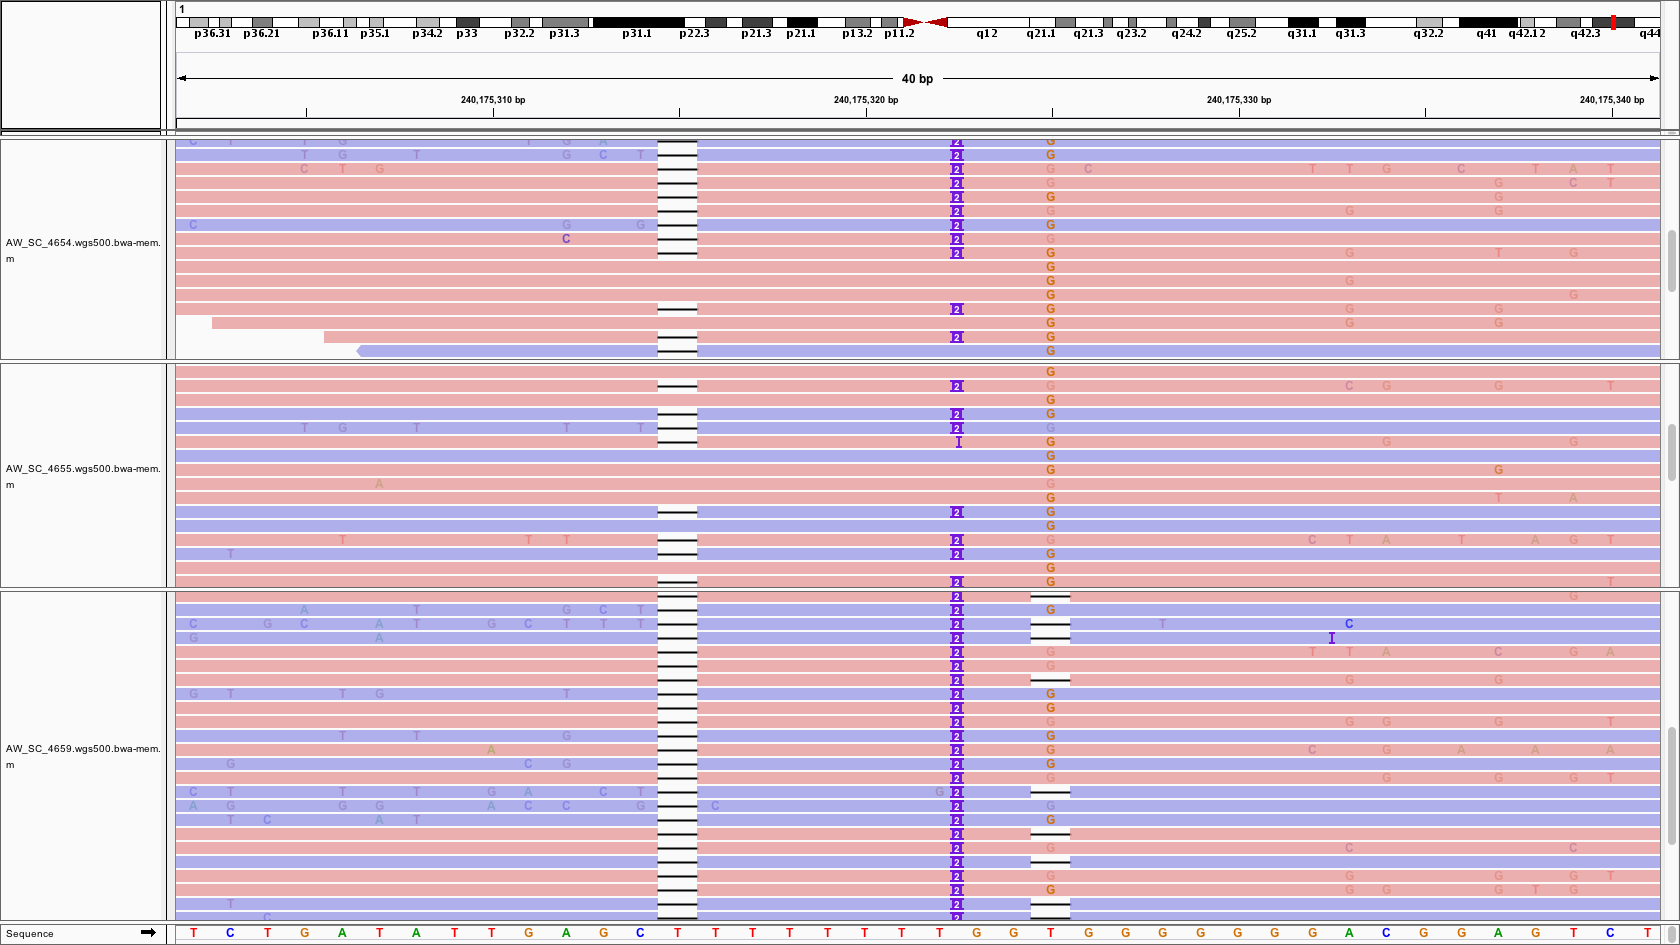
\includegraphics[width=\textwidth]{figures/1_240175324_GTdel}
        \caption{\tiny 1:240175324 GT $>$ G}
    \end{subfigure}
    \begin{subfigure}[b]{0.33\textwidth}
        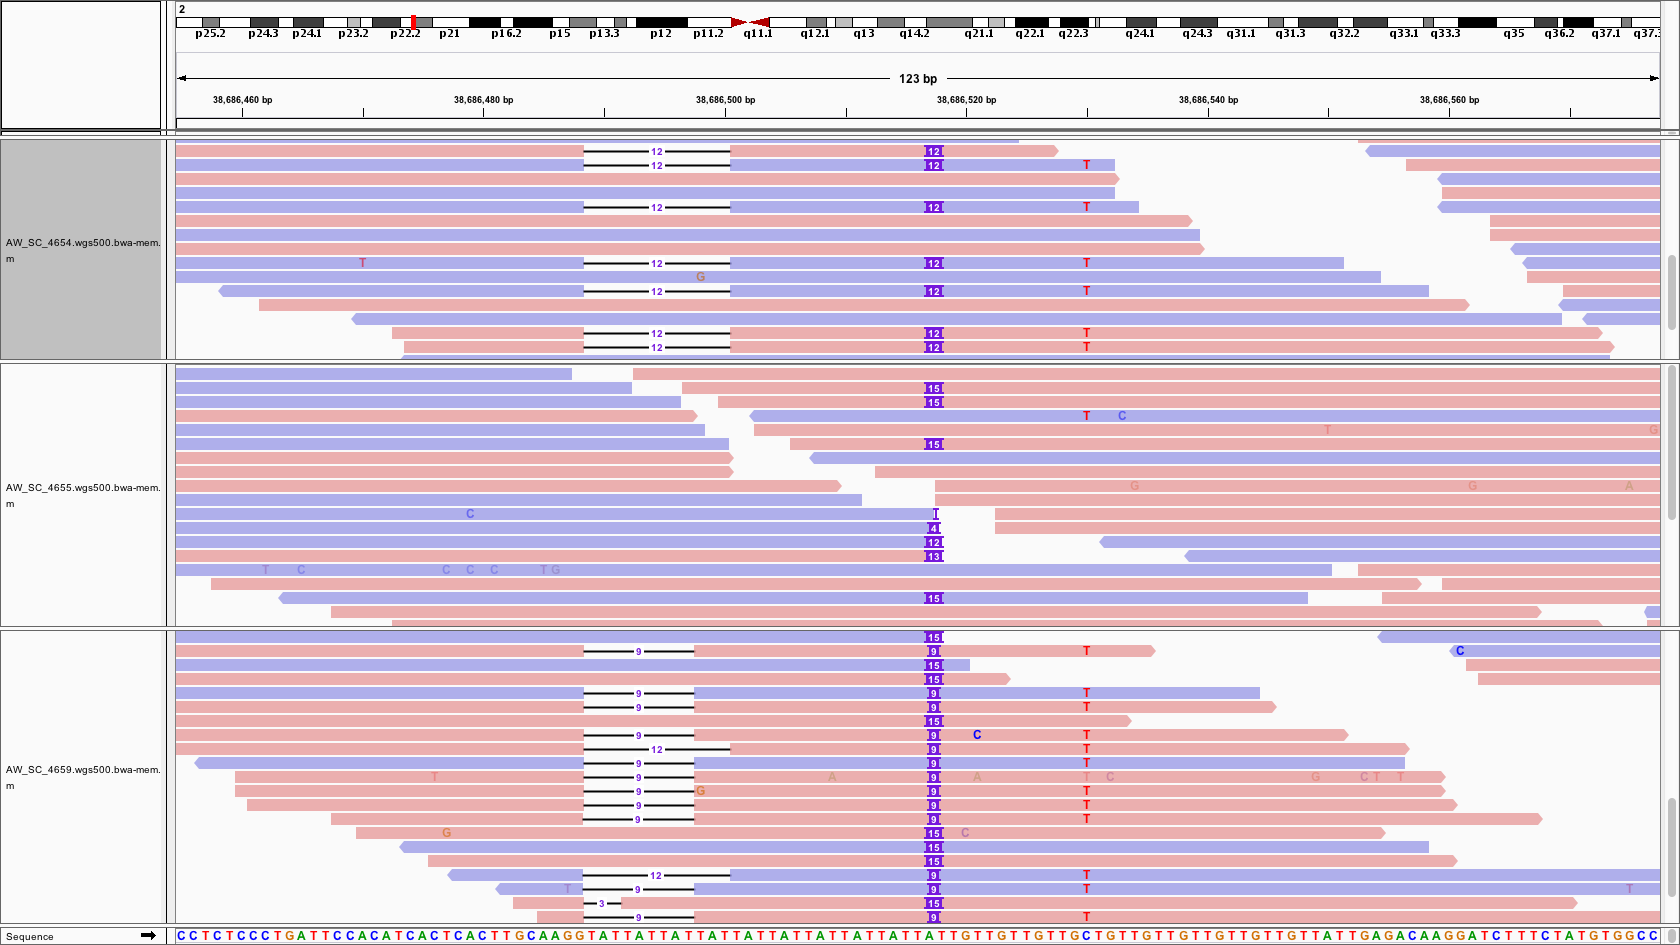
\includegraphics[width=\textwidth]{figures/2_38686488_GTATTATTATdel_38686517_ATTGTTGTTGins}
        \caption{\tiny 1:38686488 GTATTATTAT $>$ G \& 1:38686517 A $>$ ATTGTTGTTG}
    \end{subfigure}
    \begin{subfigure}[b]{0.33\textwidth}
        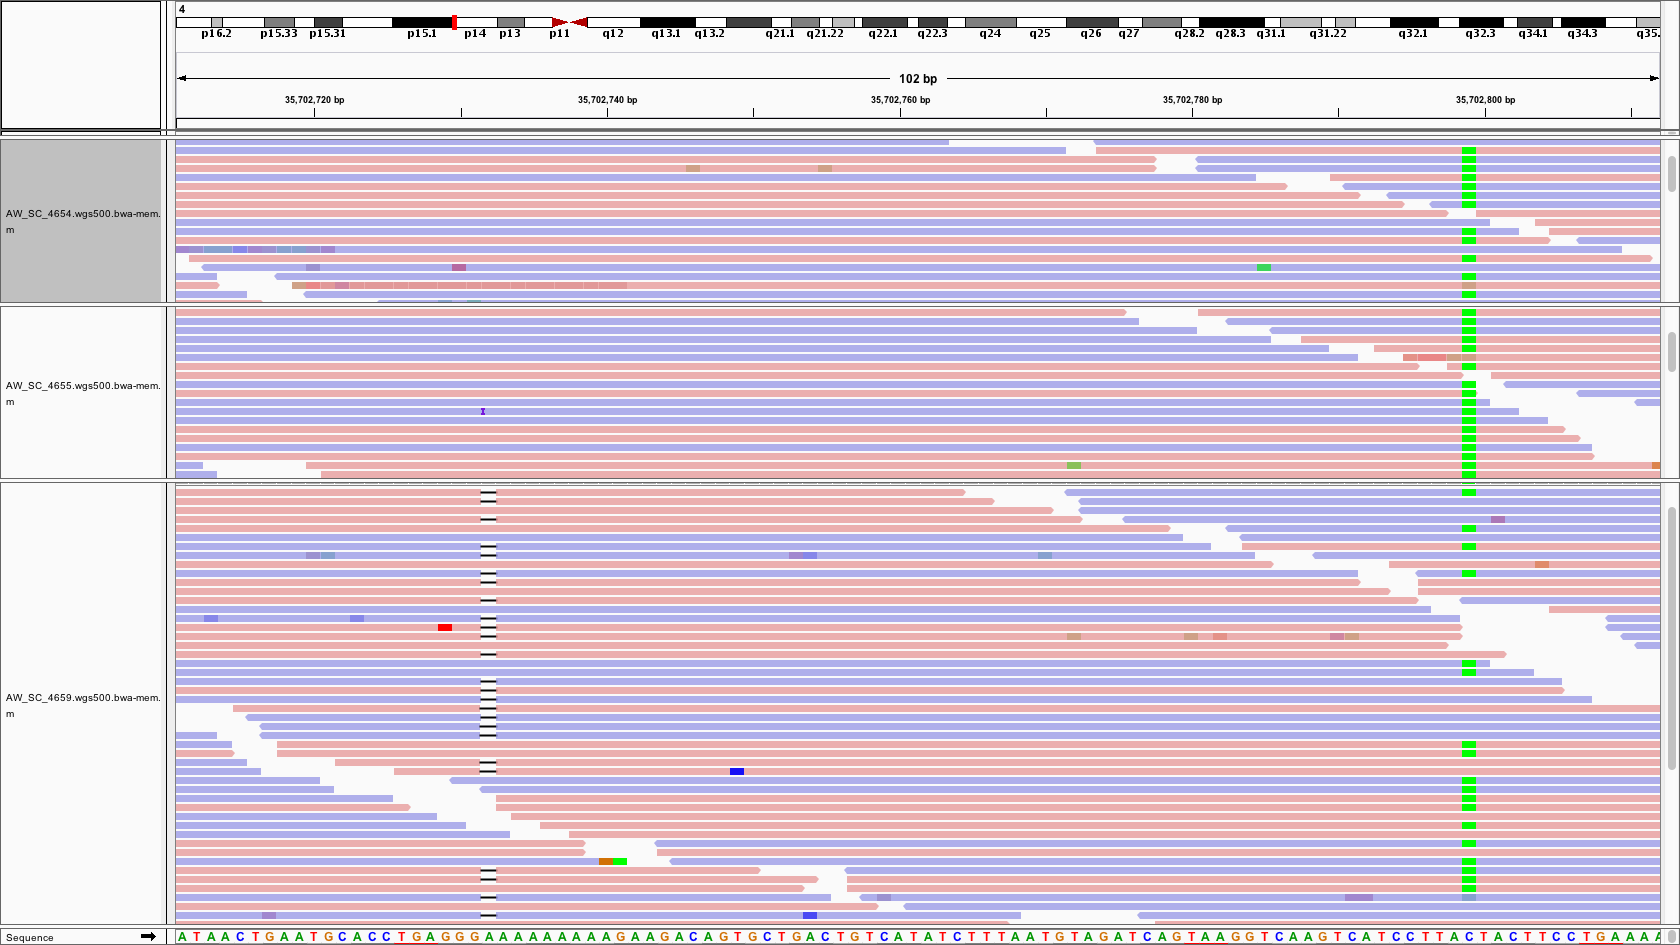
\includegraphics[width=\textwidth]{figures/4_35702731_GAdel}
        \caption{\tiny 4:35702731 GA $>$ G}
    \end{subfigure}
    \begin{subfigure}[b]{0.33\textwidth}
        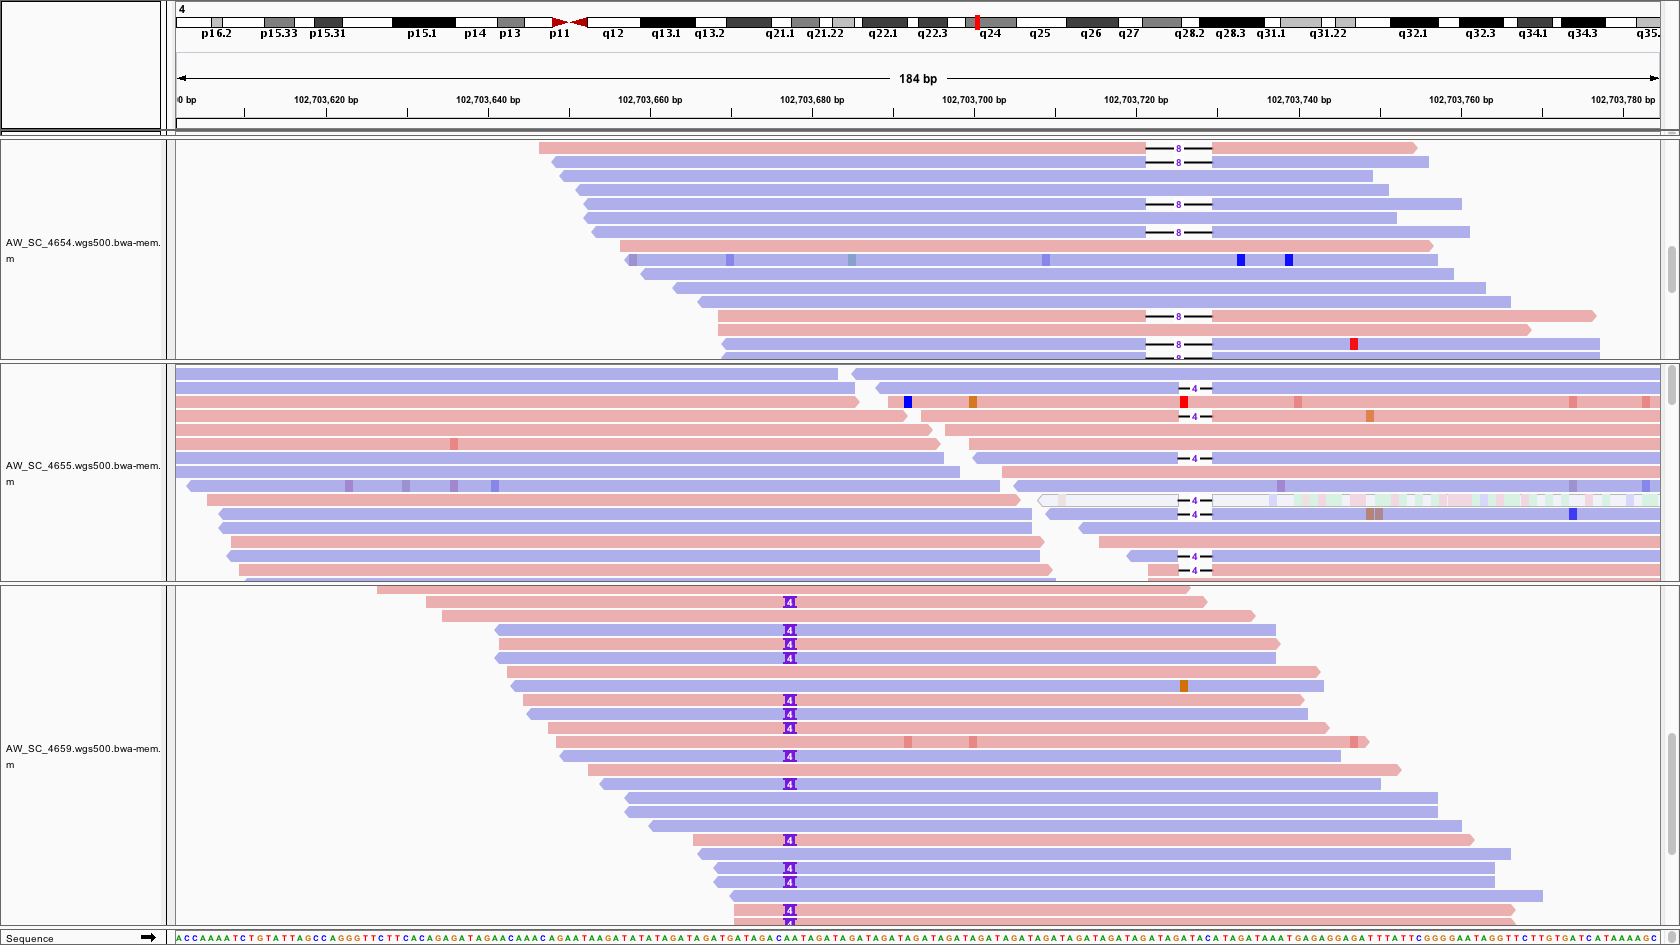
\includegraphics[width=\textwidth]{figures/4_102703677_AATAGins}
        \caption{\tiny 4:102703677 A $>$ AATAG}
    \end{subfigure}
    \begin{subfigure}[b]{0.33\textwidth}
        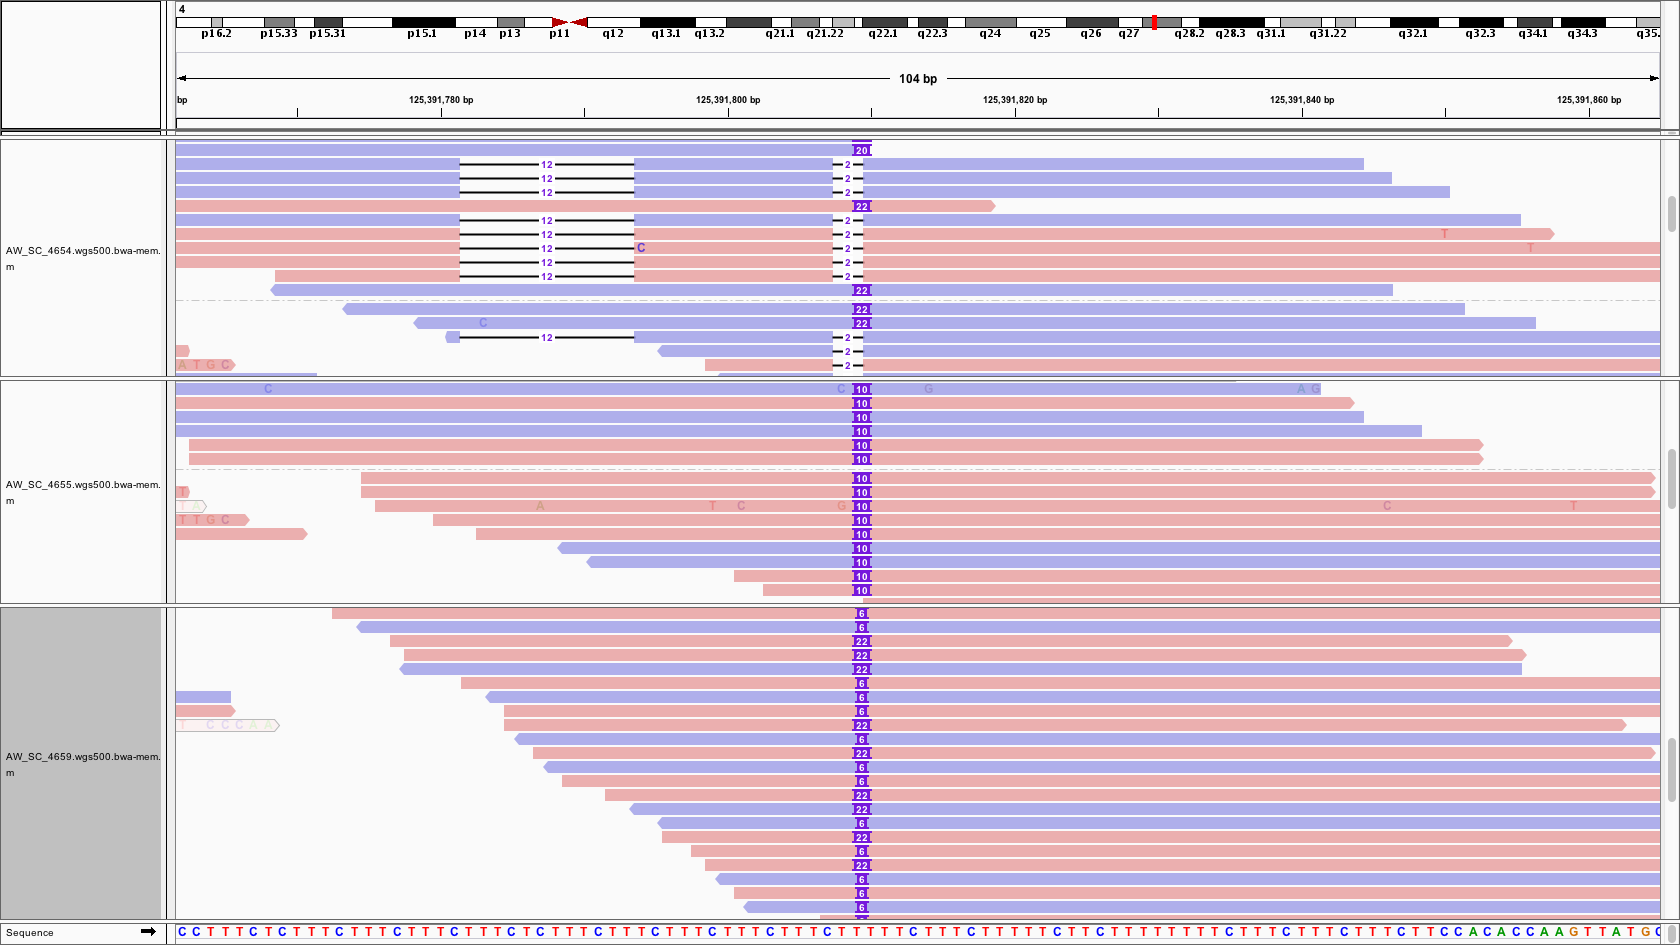
\includegraphics[width=\textwidth]{figures/4_125391809_TTCTTTCins}
        \caption{\tiny 4:125391809 T $>$ TTCTTTC}
    \end{subfigure}
    \begin{subfigure}[b]{0.33\textwidth}
        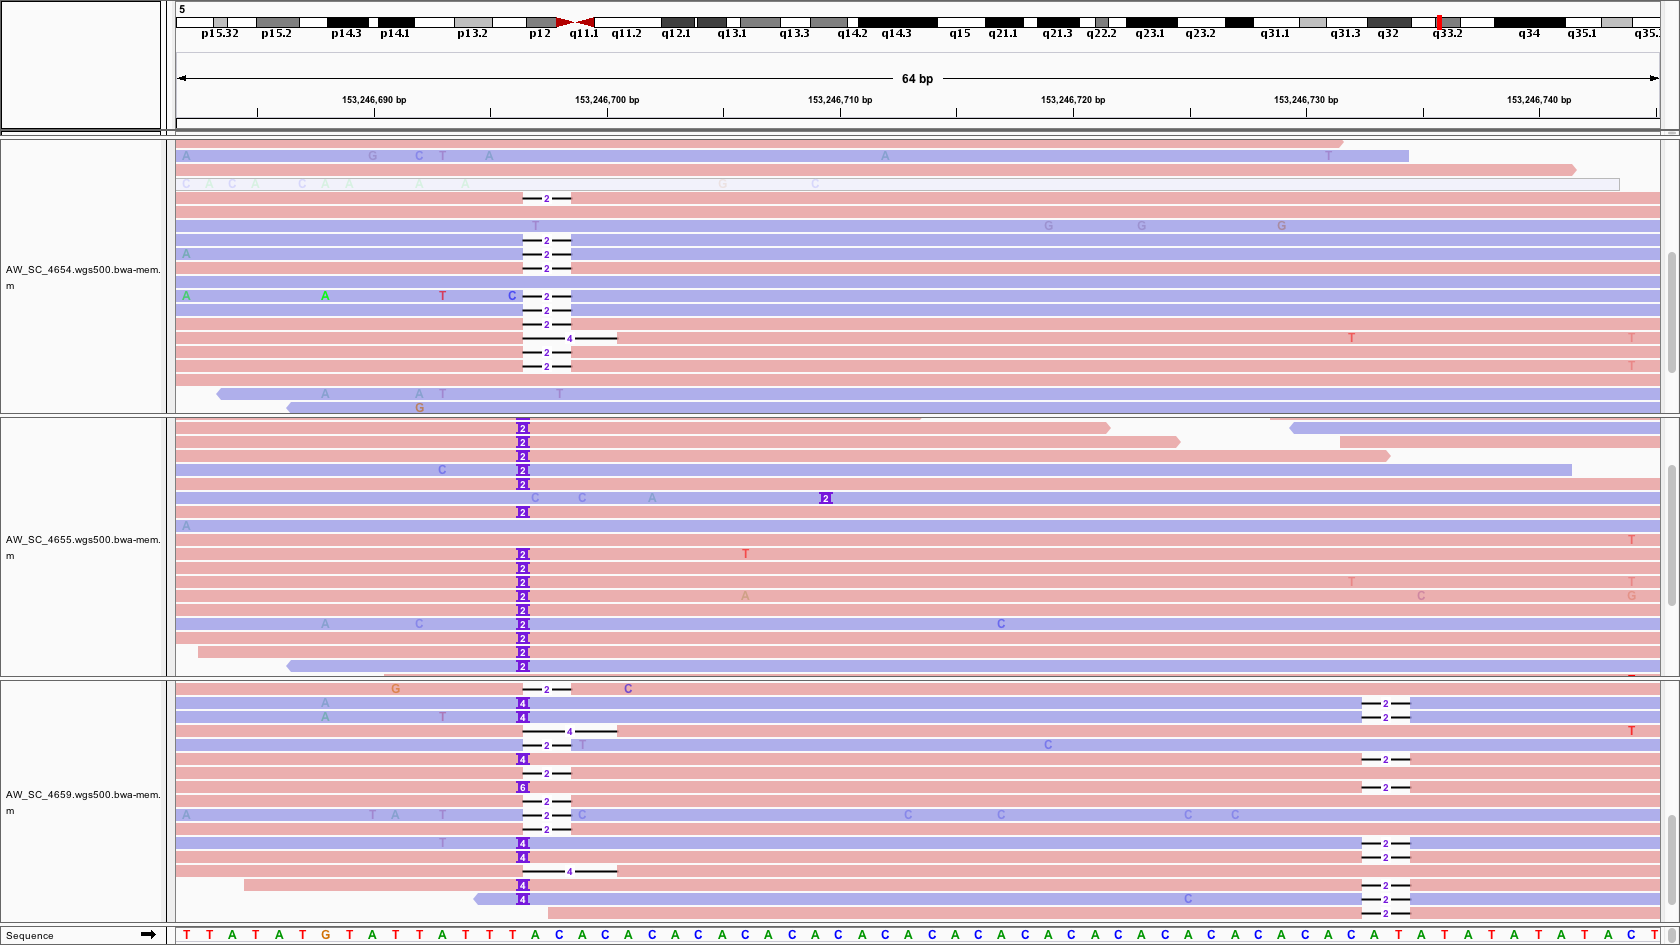
\includegraphics[width=\textwidth]{figures/5_153246696_TACACins_153246732_CATdel}
        \caption{\tiny 5:153246696 T $>$ TACAC \& 5:153246732 CAT $>$ C}
    \end{subfigure}
    \begin{subfigure}[b]{0.33\textwidth}
        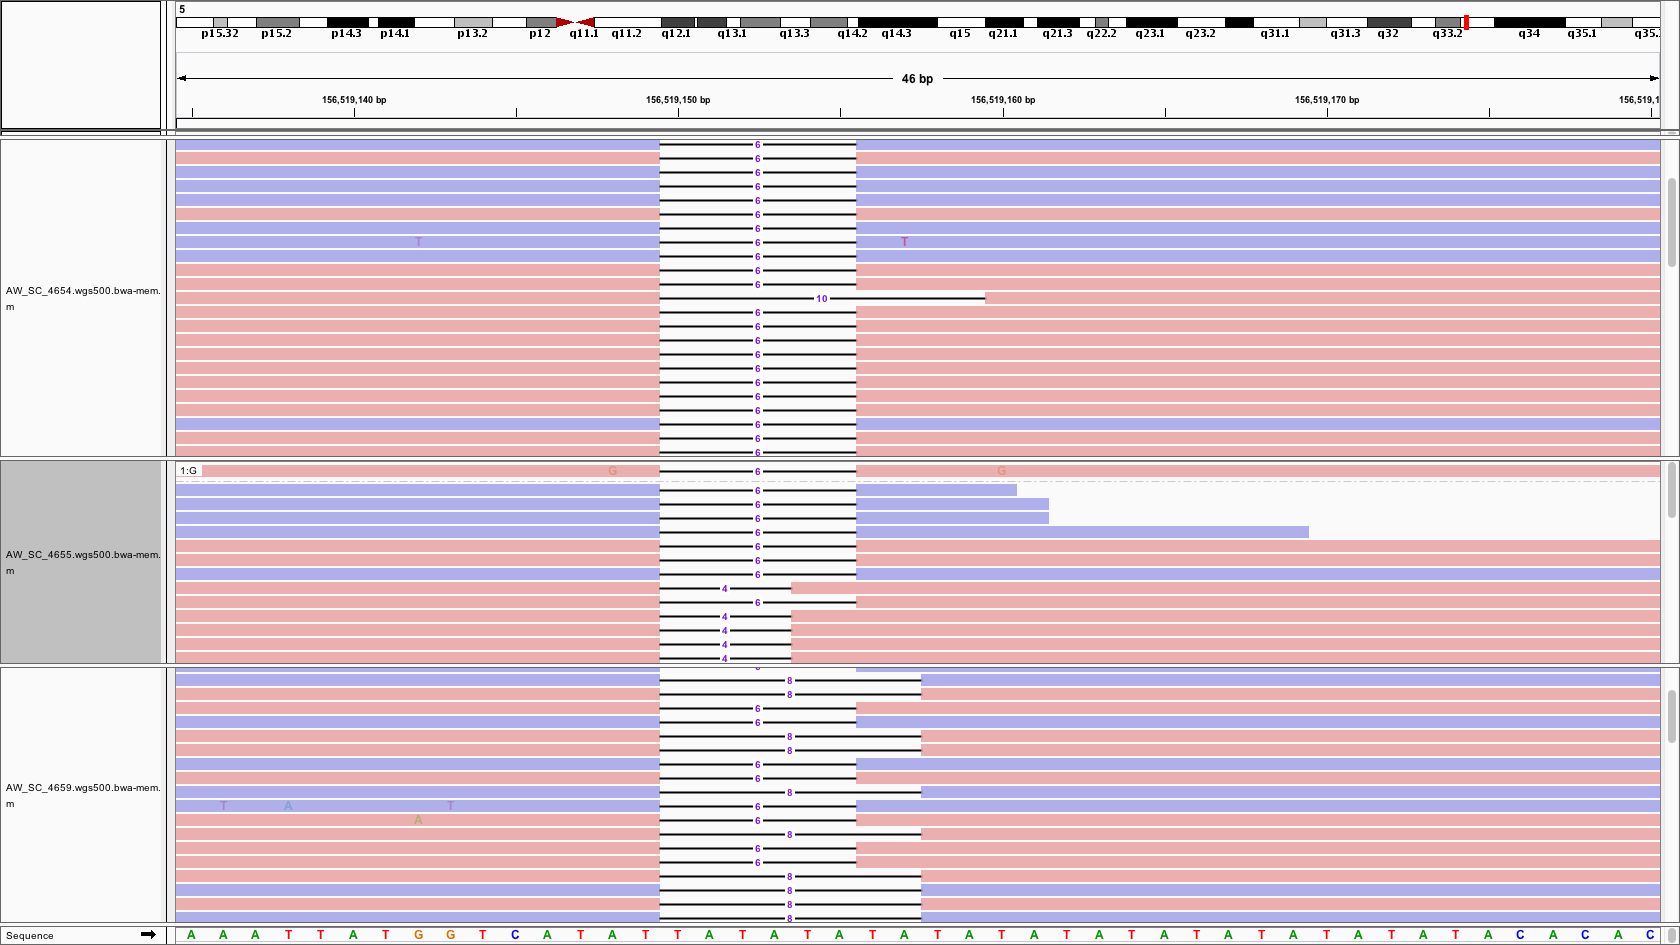
\includegraphics[width=\textwidth]{figures/5_156519149_TTATATATAdel}
        \caption{\tiny 5:156519149 TTATATATA $>$ T}
    \end{subfigure}
    \begin{subfigure}[b]{0.33\textwidth}
        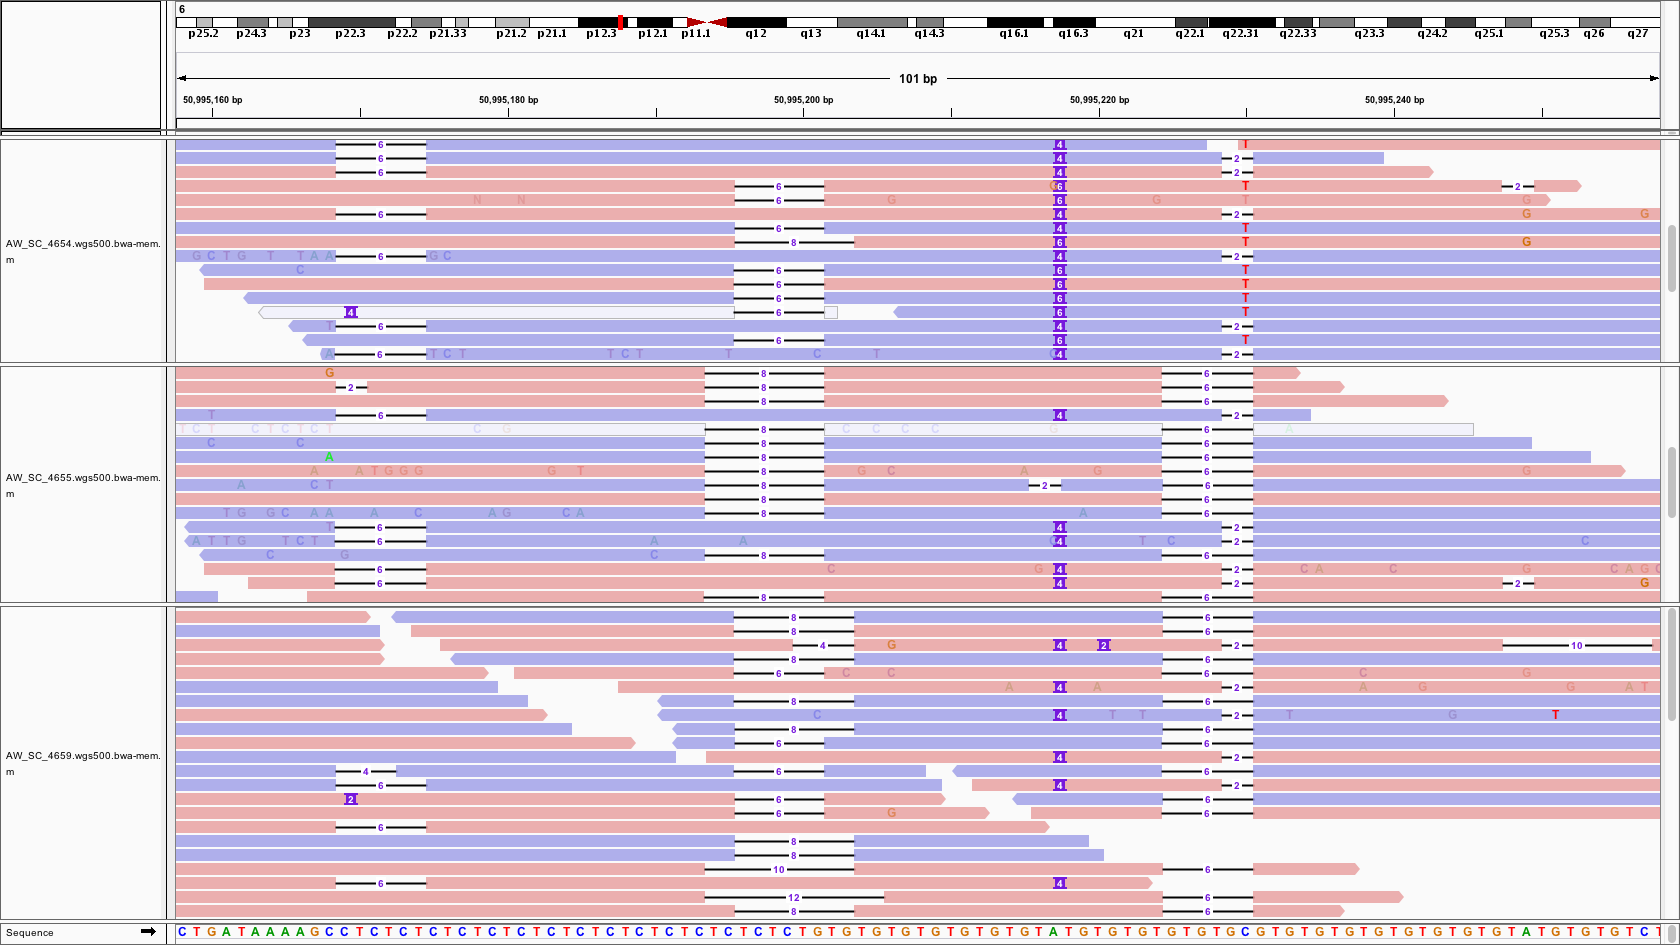
\includegraphics[width=\textwidth]{figures/6_50995195_CTCTCTGTGdel}
        \caption{\tiny 6:50995195 CTCTCTGTG $>$ C}
    \end{subfigure}
    \begin{subfigure}[b]{0.33\textwidth}
        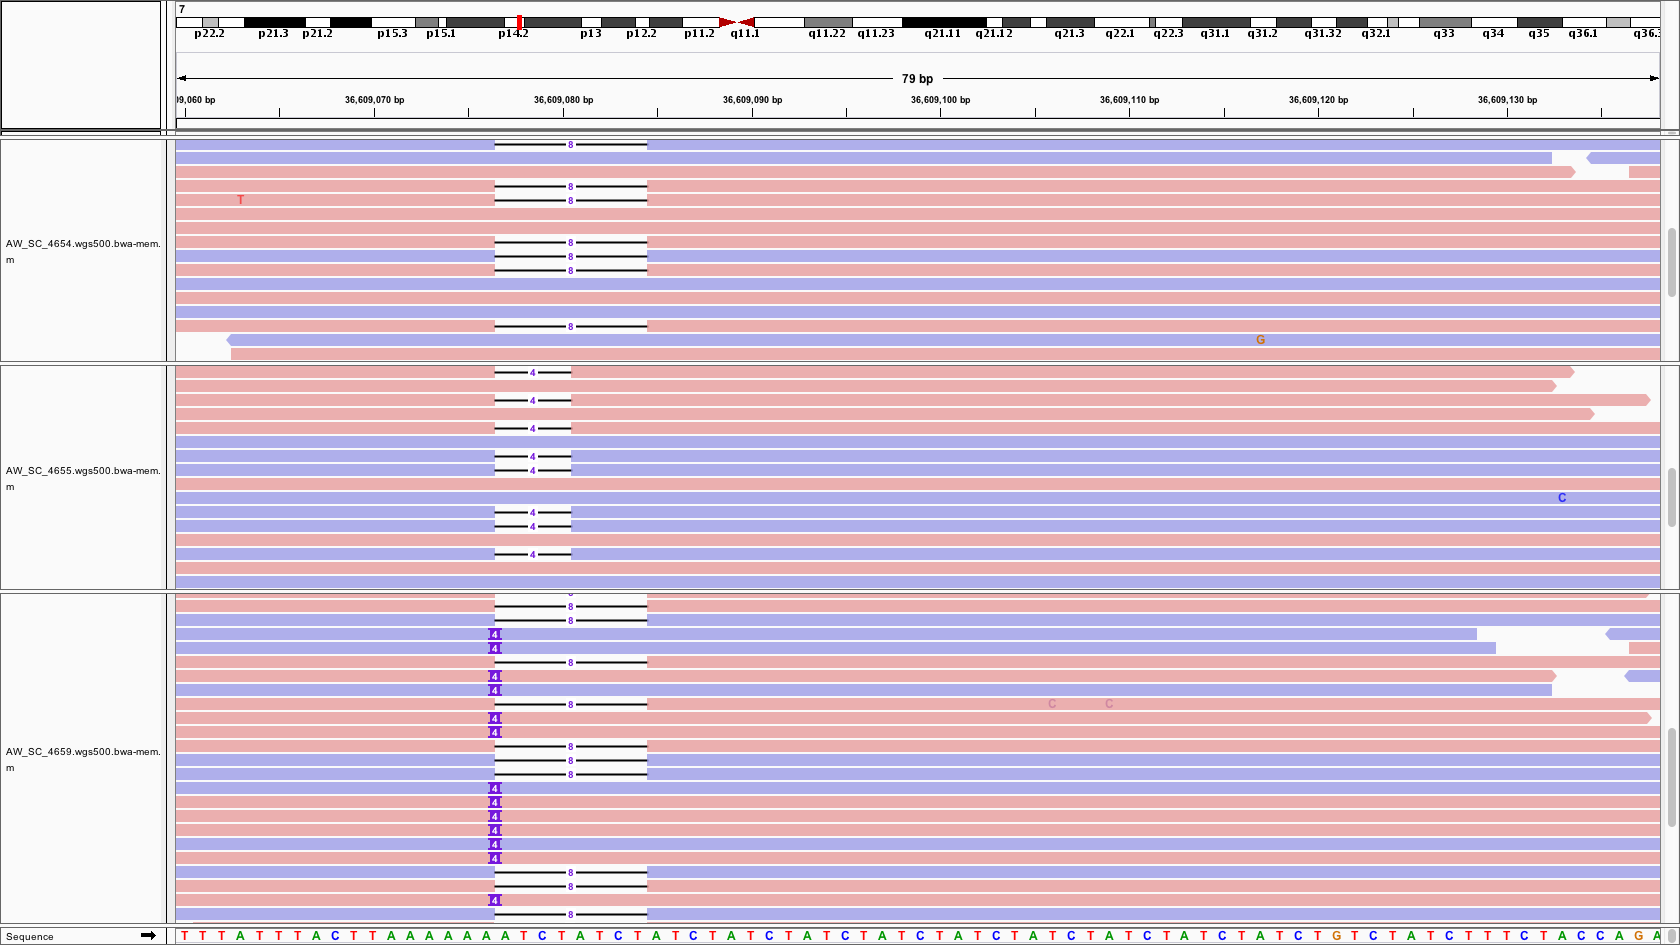
\includegraphics[width=\textwidth]{figures/7_36609076_AATCTins}
        \caption{\tiny 7:36609076 A $>$ AATCT}
    \end{subfigure}
    \begin{subfigure}[b]{0.33\textwidth}
        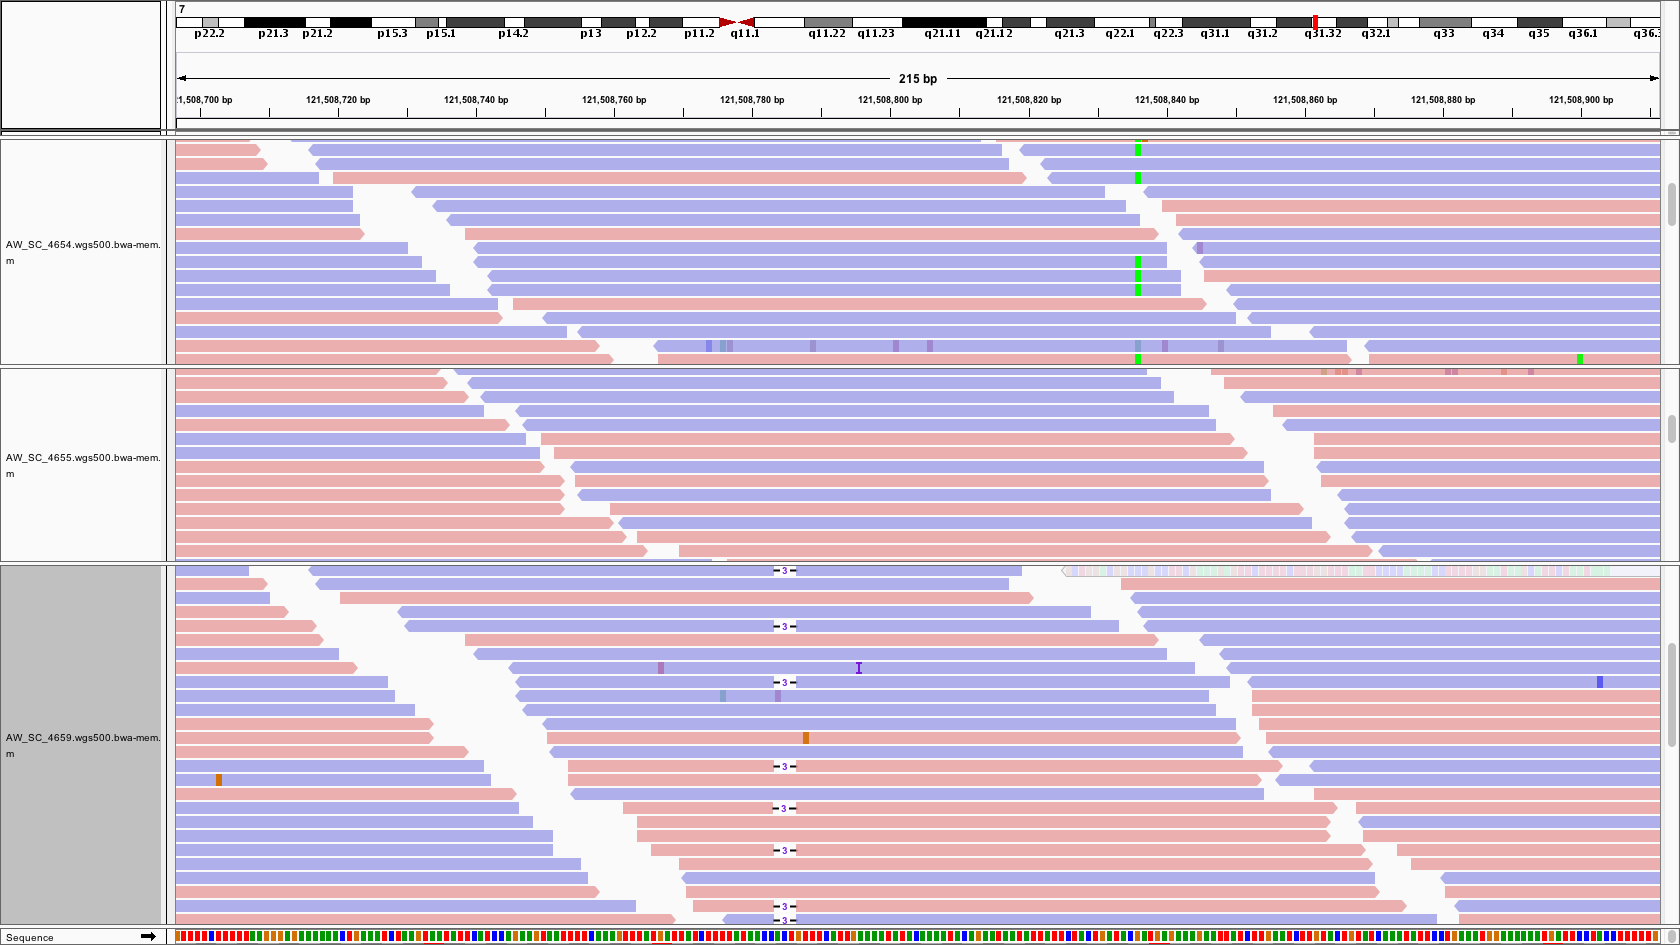
\includegraphics[width=\textwidth]{figures/7_121508783_CACTdel}
        \caption{\tiny 7:121508783 CACT $>$ C}
    \end{subfigure}
    \begin{subfigure}[b]{0.33\textwidth}
        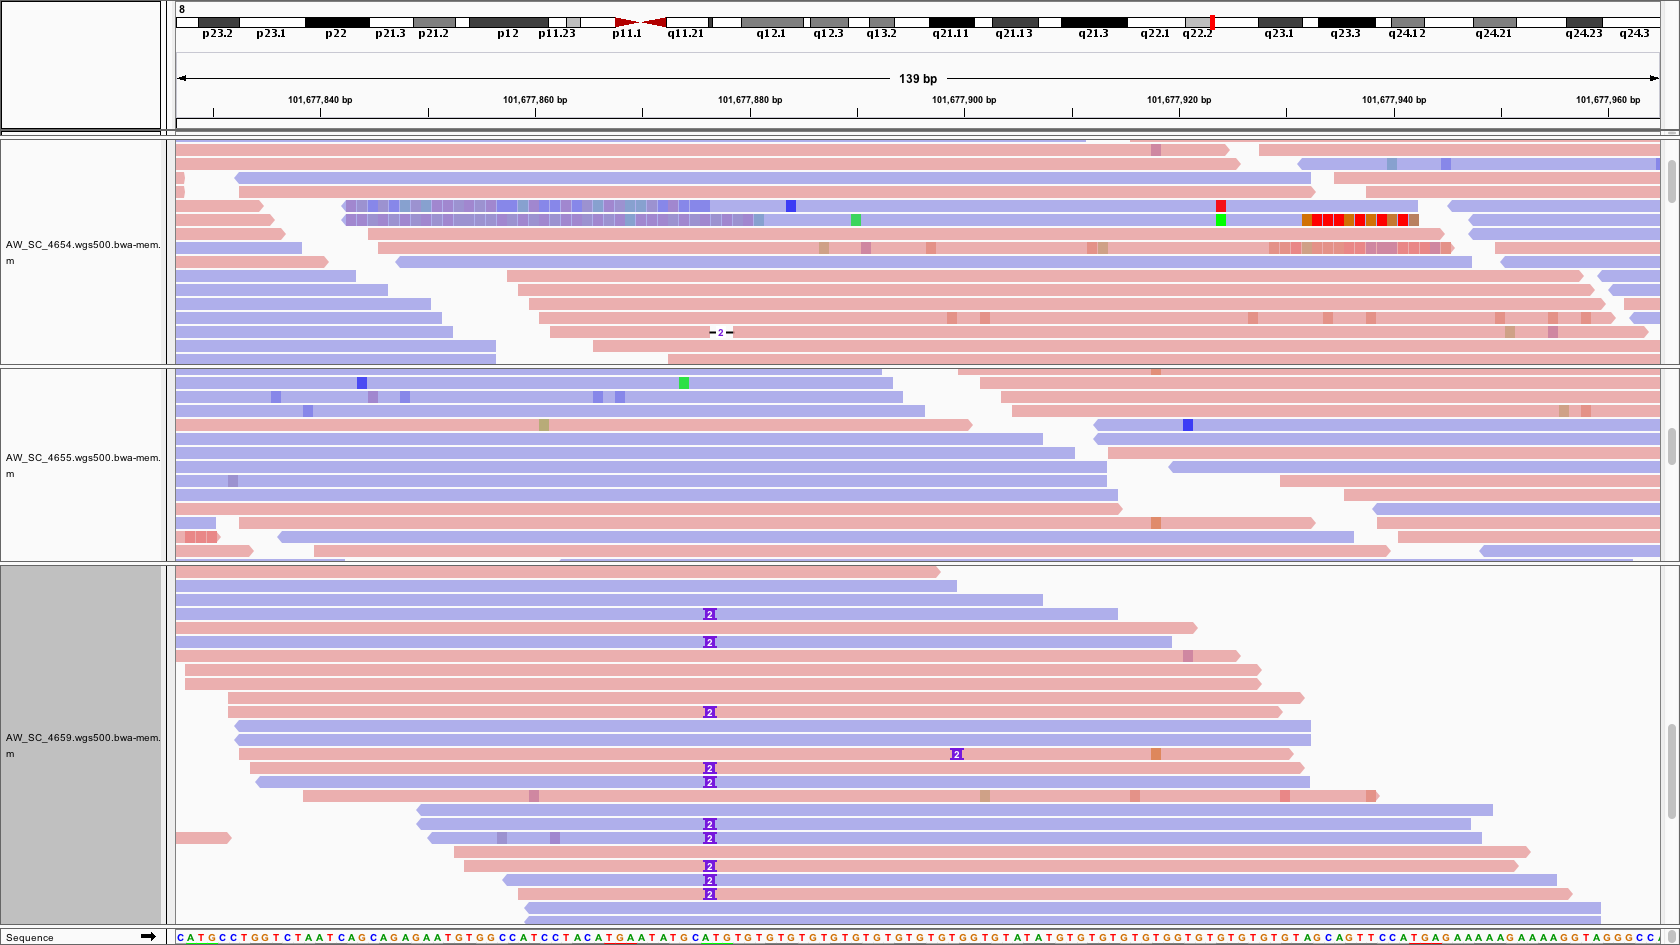
\includegraphics[width=\textwidth]{figures/8_101677876_ATGins}
        \caption{\tiny 8:101677876 A $>$ ATG}
    \end{subfigure}
    \begin{subfigure}[b]{0.33\textwidth}
        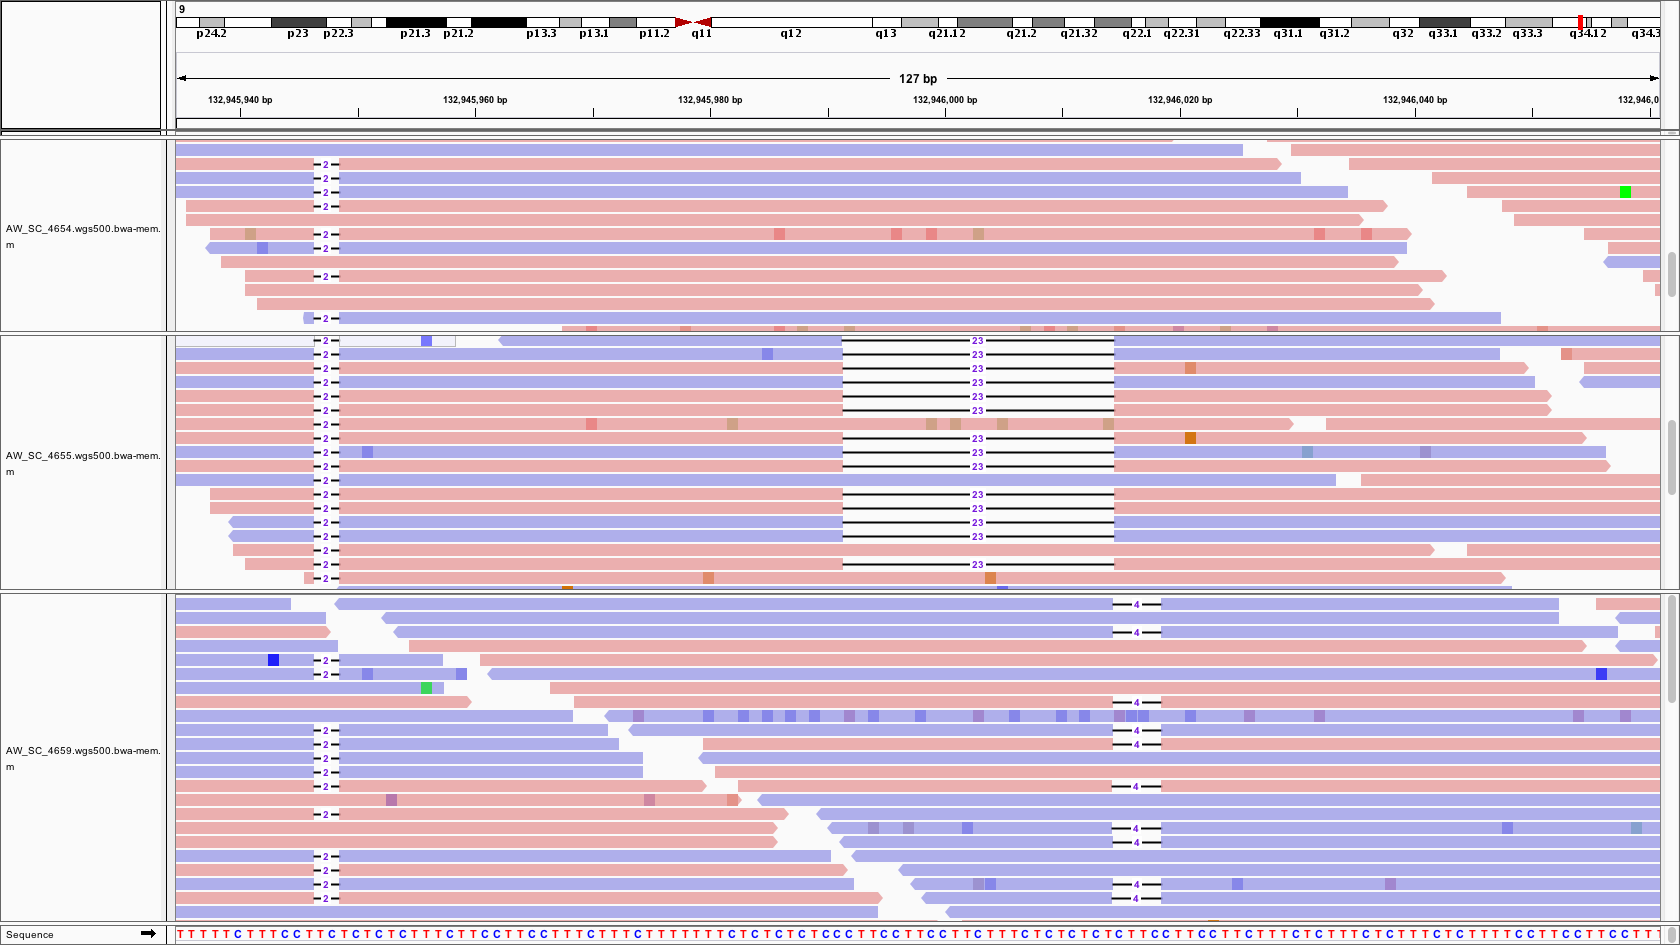
\includegraphics[width=\textwidth]{figures/9_132946014_TCTTCdel}
        \caption{\tiny 9:132946014 TCTTC $>$ T}
    \end{subfigure}
    \begin{subfigure}[b]{0.33\textwidth}
        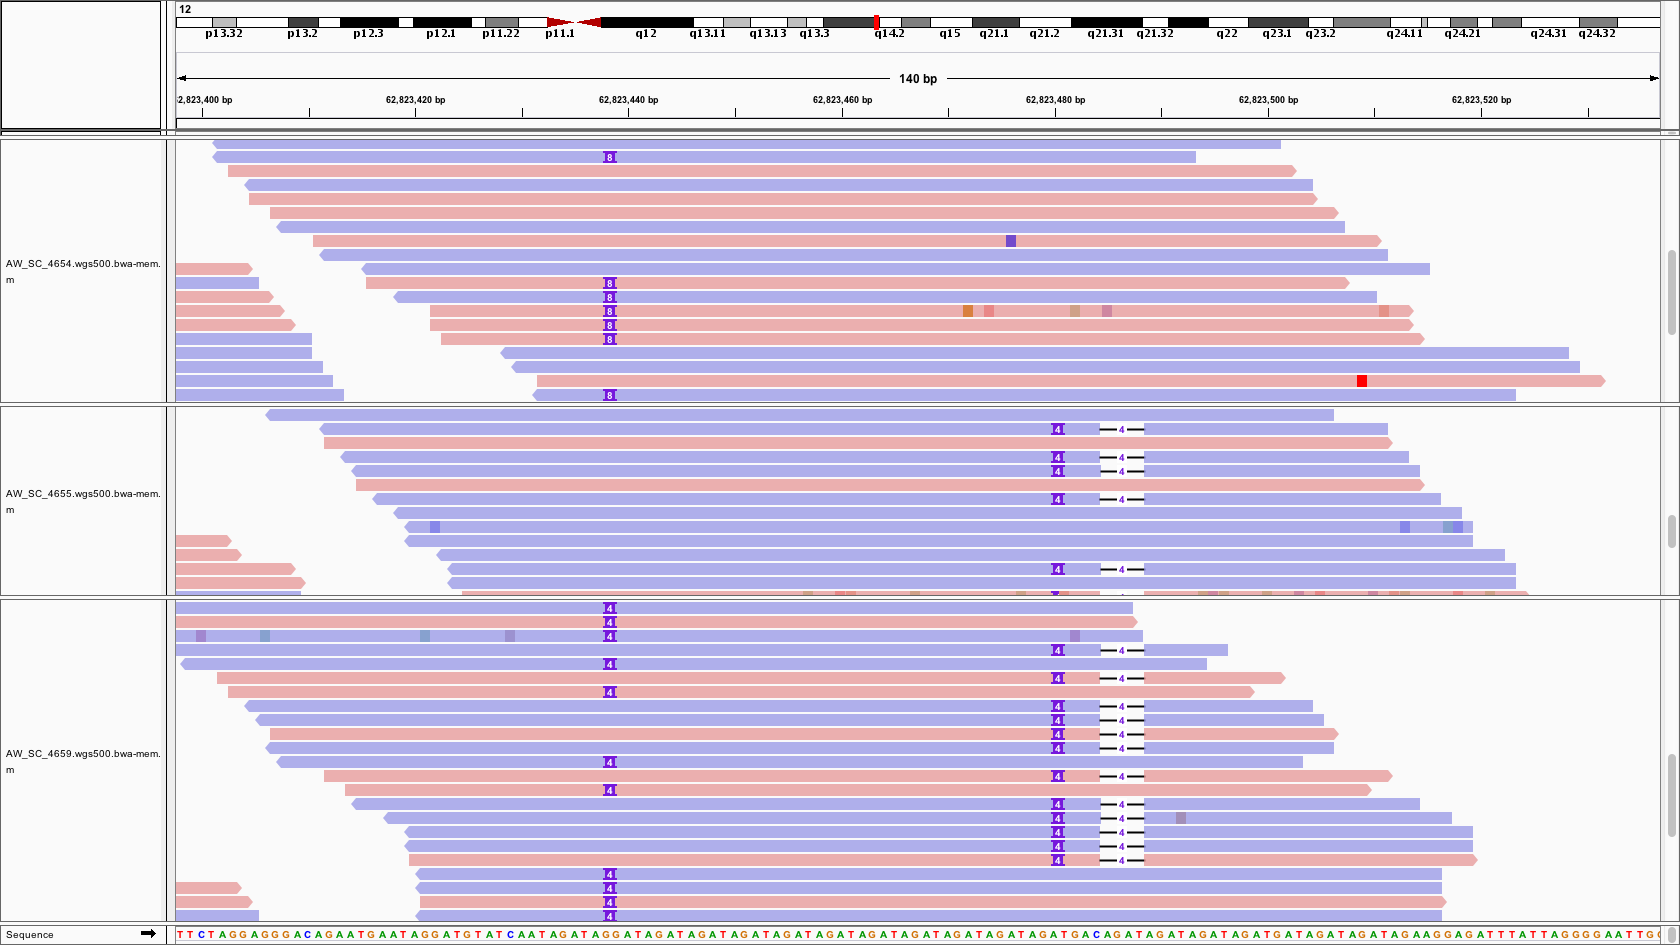
\includegraphics[width=\textwidth]{figures/12_62823438_GGATAins}
        \caption{\tiny 12:62823438 G $>$ GGATA}
    \end{subfigure}
    \begin{subfigure}[b]{0.33\textwidth}
        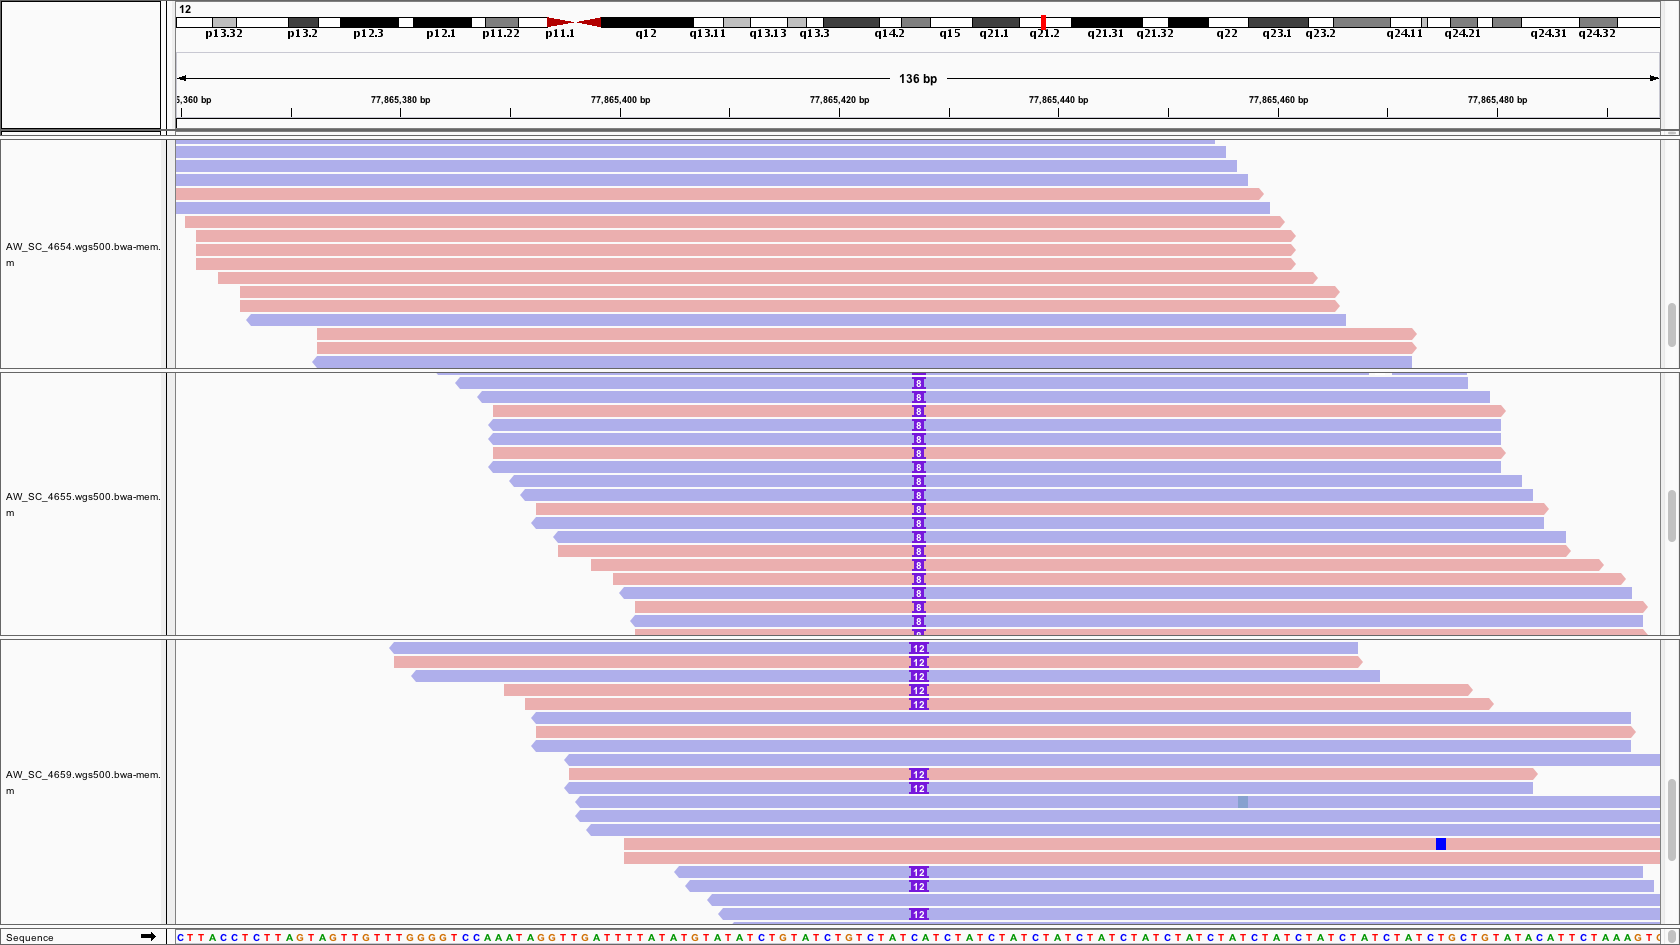
\includegraphics[width=\textwidth]{figures/12_77865427_CATCTATCTATCTins}
        \caption{\tiny 12:77865427 C $>$ CATCTATCTATCT}
    \end{subfigure}
    \begin{subfigure}[b]{0.33\textwidth}
        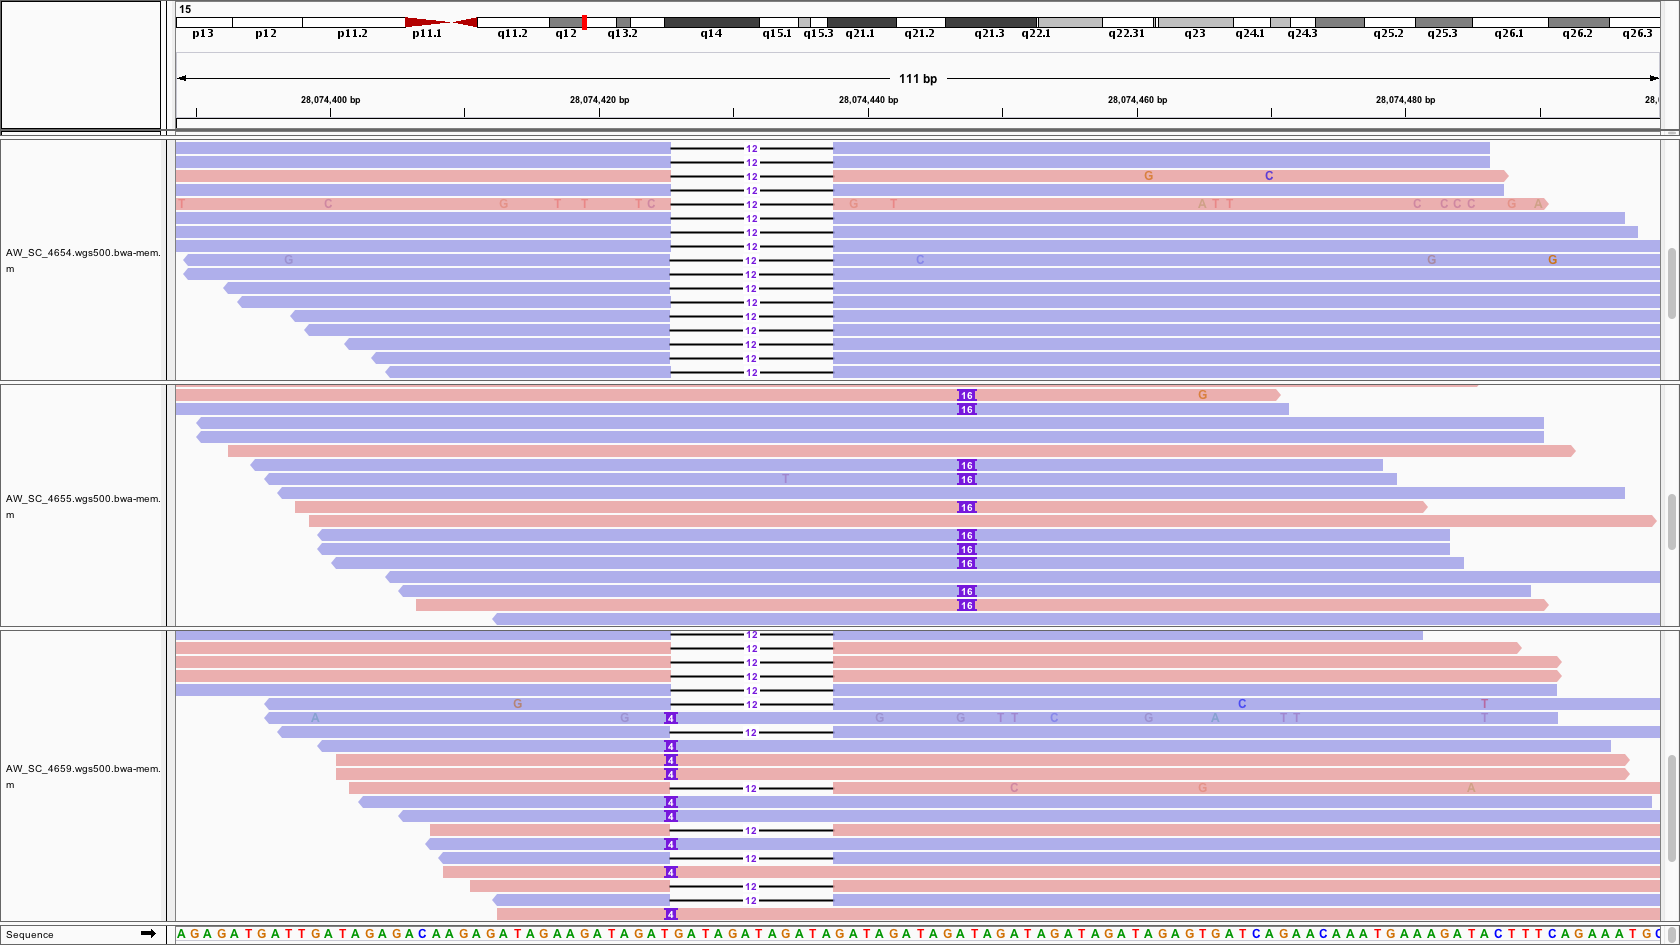
\includegraphics[width=\textwidth]{figures/15_28074425_TGATAins}
        \caption{\tiny 15:28074425 T $>$ TGATA}
    \end{subfigure}
    \caption{Octopus evidence BAM realignments for curated indel \textit{de novo} mutations. Realigned reads are shown for parents (top two panels) and offspring (bottom panel).}.
    \label{subfig:denovo-realignments}
\end{figure*}

\end{landscape}

\clearpage

\begin{figure*}[ht!]
    \centering
    \begin{subfigure}[b]{0.49\textwidth}
        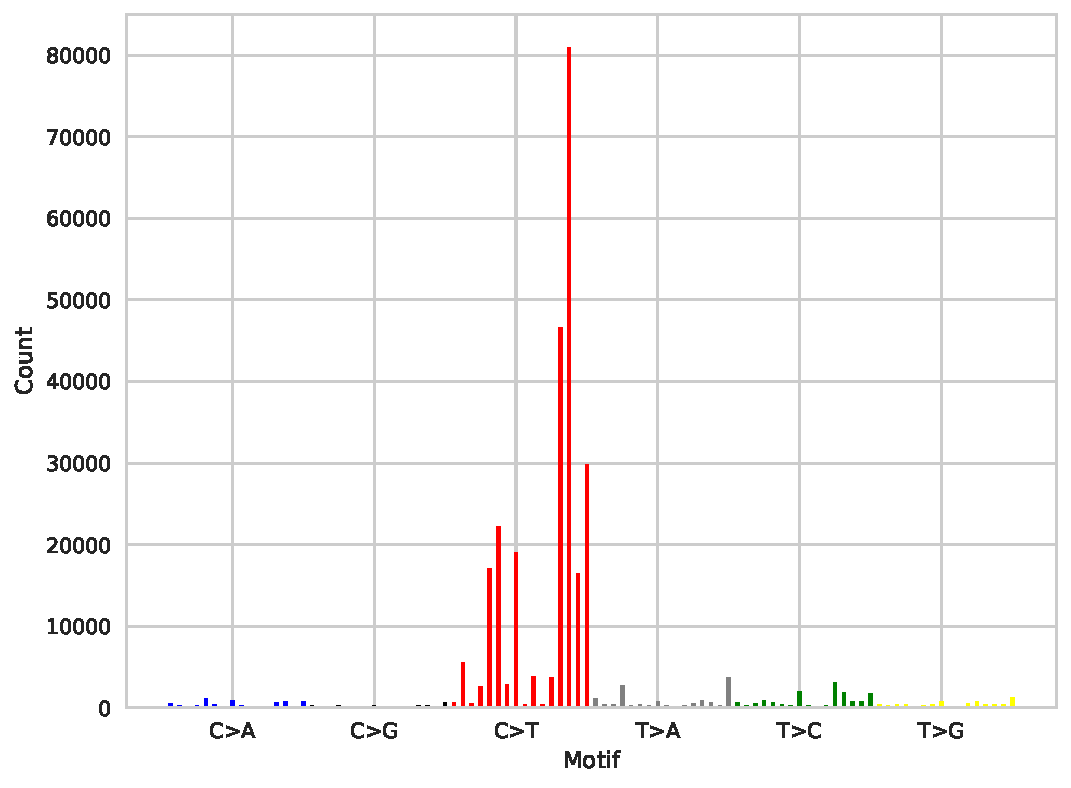
\includegraphics[width=\textwidth]{figures/synthetic_skin_tumour_snvs}
        \caption{}
        \label{supfig:synthetic-skin-snv}
    \end{subfigure}
    \hfill
    \begin{subfigure}[b]{0.49\textwidth}
        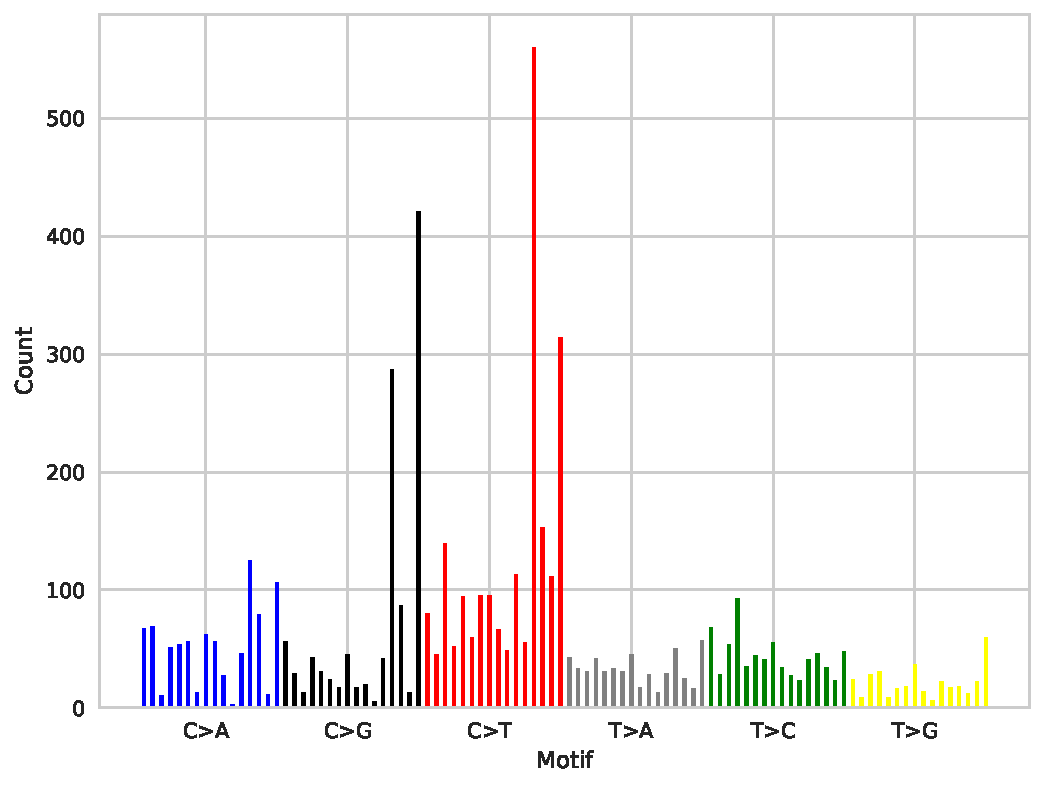
\includegraphics[width=\textwidth]{figures/synthetic_breast_tumour_snvs}
        \caption{}
        \label{supfig:synthetic-breast-snv}
    \end{subfigure}
    \hfill
    \begin{subfigure}[b]{0.49\textwidth}
        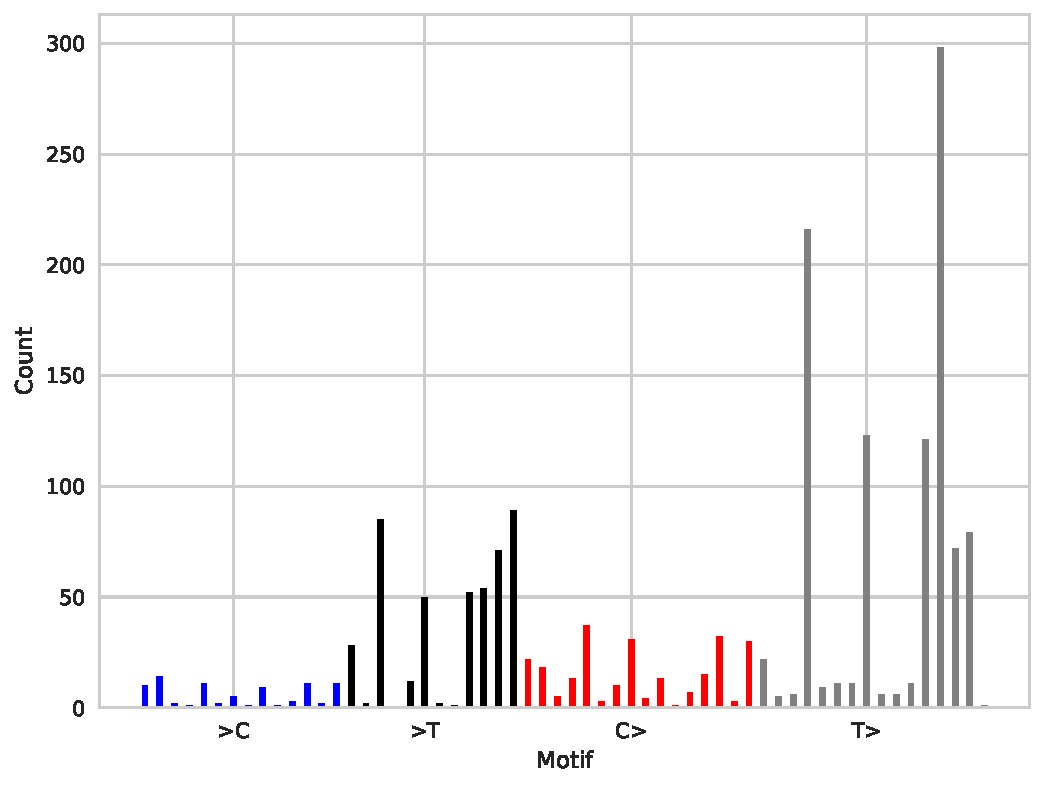
\includegraphics[width=\textwidth]{figures/synthetic_skin_tumour_1bp_indels}
        \caption{}
        \label{supfig:synthetic-skin-indel}
    \end{subfigure}
    \begin{subfigure}[b]{0.49\textwidth}
        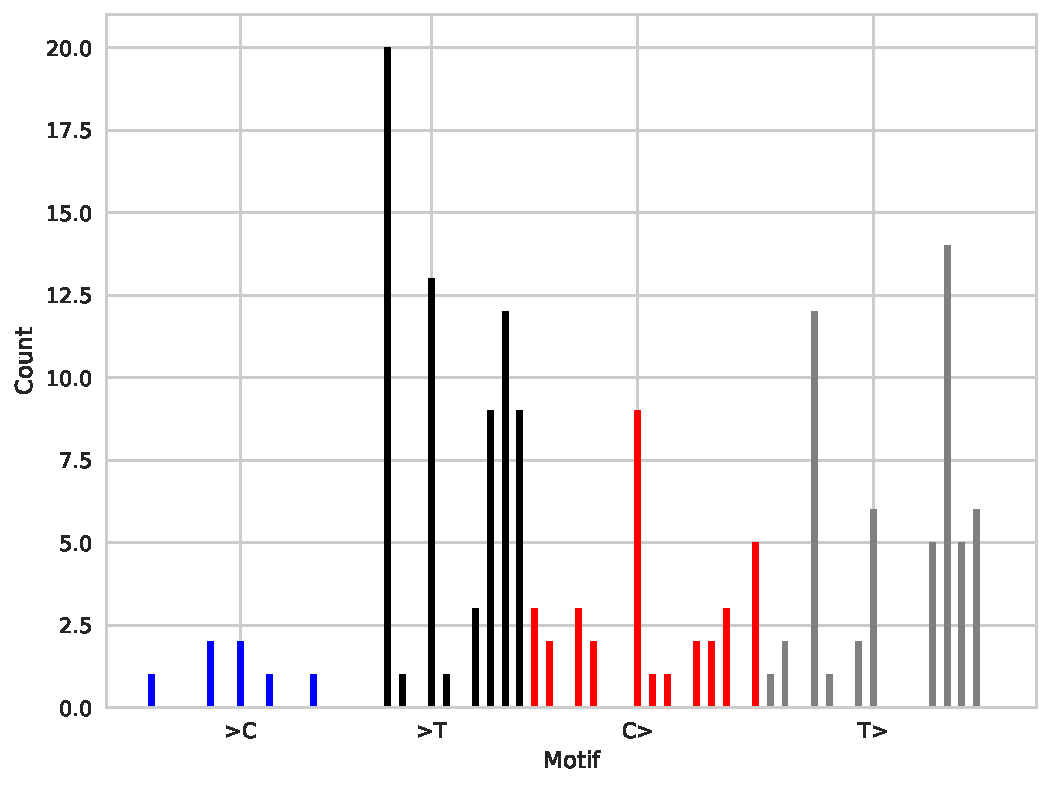
\includegraphics[width=\textwidth]{figures/synthetic_breast_tumour_1bp_indels}
        \caption{}
        \label{supfig:synthetic-breast-indel}
    \end{subfigure}
    \hfill
    \begin{subfigure}[b]{0.49\textwidth}
        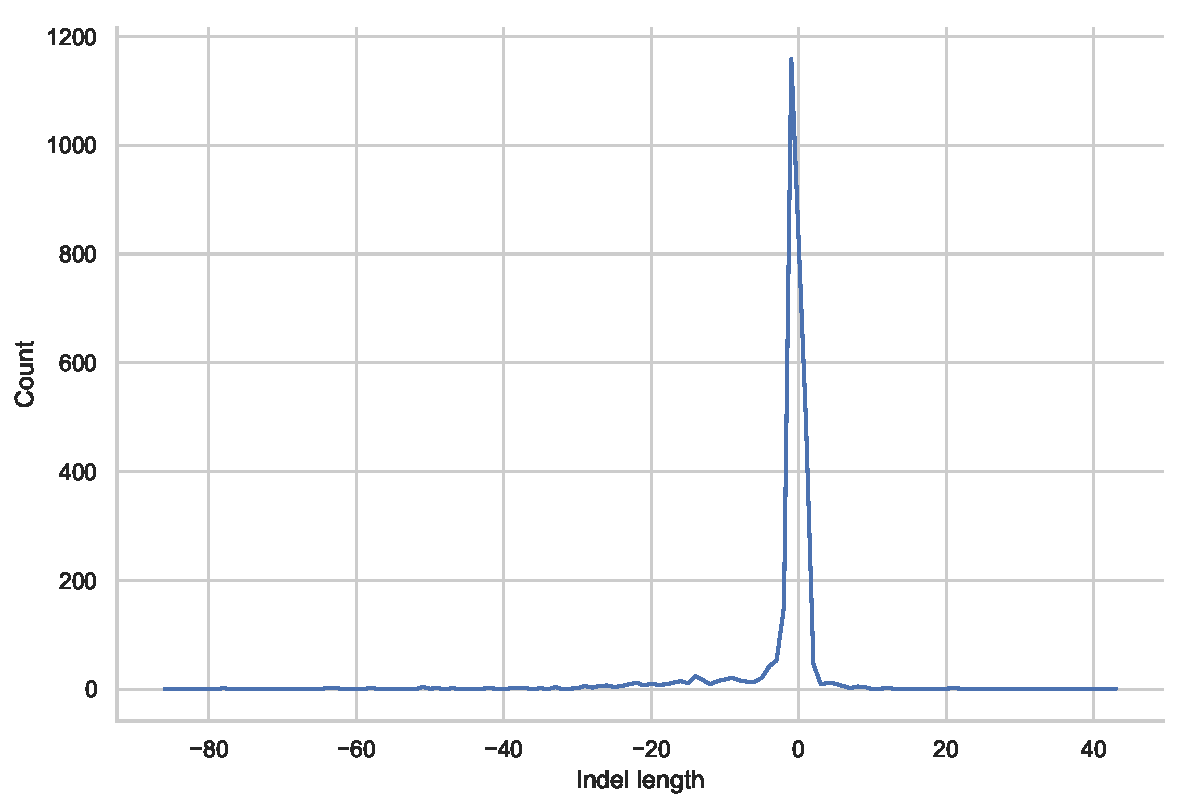
\includegraphics[width=\textwidth]{figures/synthetic_skin_spike_indels}
        \caption{}
        \label{supfig:synthetic-skin-indel-size}
    \end{subfigure}
    \begin{subfigure}[b]{0.49\textwidth}
        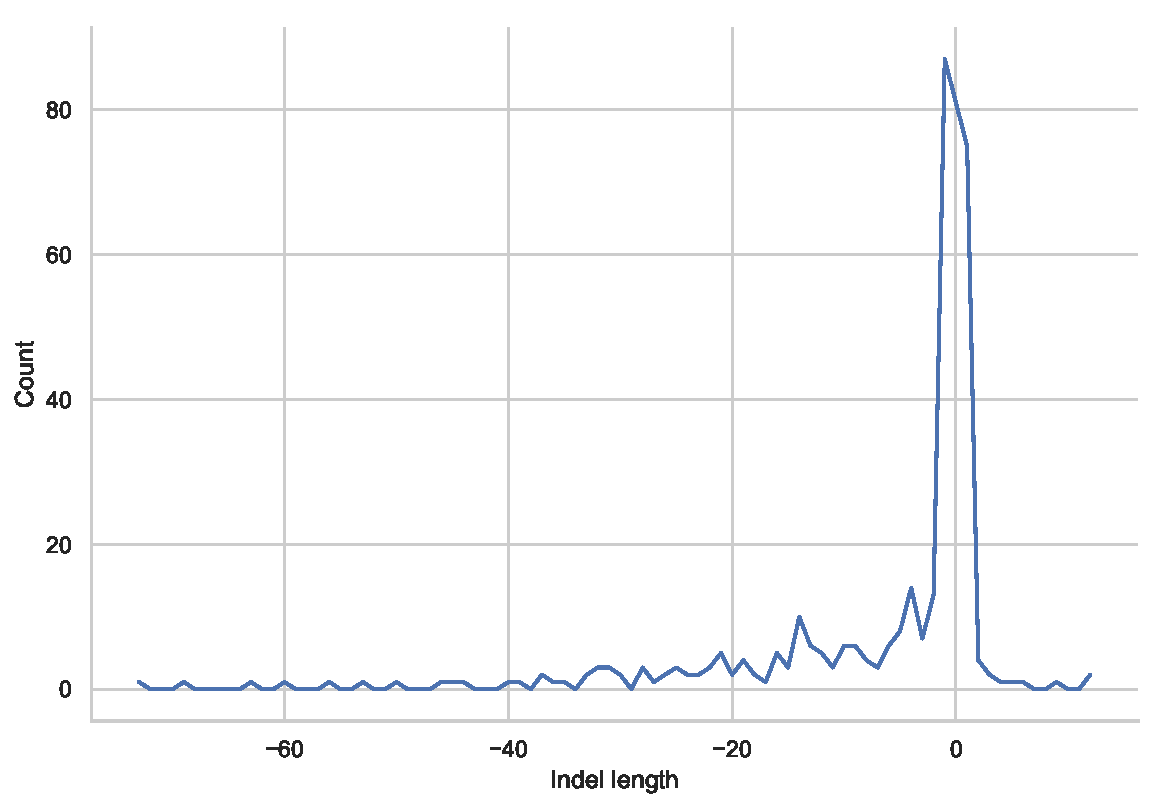
\includegraphics[width=\textwidth]{figures/synthetic_breast_spike_indels}
        \caption{}
        \label{supfig:synthetic-breast-indel-size}
    \end{subfigure}
    \caption{Mutation profiles of synthetic tumours. \textbf{\subref{supfig:synthetic-skin-snv}}, \textbf{\subref{supfig:synthetic-breast-snv}} show the SNV distribution with $1$ bp context in the synthetic skin tumour (left) and synthetic breast tumour (right). \textbf{\subref{supfig:synthetic-skin-indel}}, \textbf{\subref{supfig:synthetic-breast-indel}} show the $1$ bp indel distribution with $1$ bp context in the synthetic skin tumour (left) and synthetic breast tumour (right). \textbf{\subref{supfig:synthetic-skin-indel-size}}, \textbf{\subref{supfig:synthetic-breast-indel-size}} show the size distribution of indels in the synthetic skin tumour (left) and synthetic breast tumour (right).} 
    \label{supfig:synthetic-tumours}
\end{figure*}

\clearpage

\begin{figure}[ht!]
    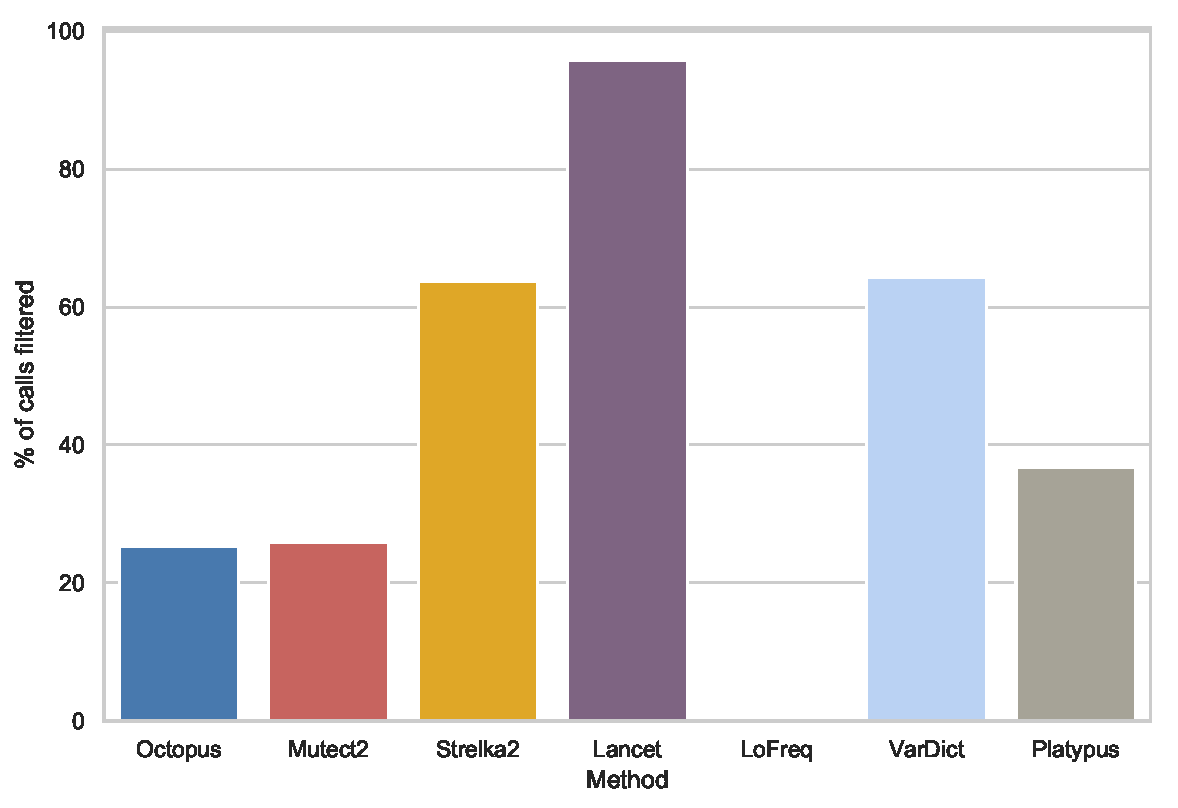
\includegraphics[width=\textwidth]{figures/filtering}
    \caption{Proportion of somatic calls filtered for the paired synthetic skin (N:30x T:60x).}
    \label{supfig:filtering}
\end{figure}

\clearpage

\begin{table}[ht!]
    \centering
    \caption{Paired somatic benchmarks summary.}
    \label{suptable:paired-somatic}
    \small
    \sffamily
    \resizebox{\linewidth}{!}{%
    \begin{tabular}{lrrllllllll}
\toprule
   Tumour &  Normal depth &  Tumour depth &    Caller & True-pos-baseline & True-pos-call & False-pos & False-neg & Precision & Sensitivity & F-measure \\
\midrule
   skin &            15 &            60 &   Octopus &            251710 &        251720 &      4467 &     29586 &    0.9826 &      0.8948 &    0.9366 \\
   skin &            15 &            60 &   Mutect2 &            238088 &        238087 &      3344 &     43208 &    0.9861 &      0.8464 &    0.9109 \\
   skin &            15 &            60 &  Strelka2 &            234156 &        234155 &      3345 &     47140 &    0.9859 &      0.8324 &    0.9027 \\
   skin &            15 &            60 &    Lancet &            200337 &        200337 &      1767 &     80959 &    0.9913 &      0.7122 &    0.8289 \\
   skin &            15 &            60 &    LoFreq &            199181 &        199181 &       418 &     82115 &    0.9979 &      0.7081 &    0.8284 \\
   skin &            15 &            60 &   VarDict &            253293 &        253292 &     60745 &     28003 &    0.8066 &      0.9005 &    0.8509 \\
   skin &            15 &            60 &  Platypus &             69530 &         69530 &      1235 &    211766 &    0.9825 &      0.2472 &    0.3950 \\
   skin &            30 &            30 &   Octopus &            231214 &        231221 &      3689 &     50082 &    0.9843 &      0.8220 &    0.8958 \\
   skin &            30 &            30 &   Mutect2 &            219304 &        219304 &      1322 &     61992 &    0.9940 &      0.7796 &    0.8739 \\
   skin &            30 &            30 &  Strelka2 &            212106 &        212106 &      1460 &     69190 &    0.9932 &      0.7540 &    0.8572 \\
   skin &            30 &            30 &    Lancet &            186781 &        186781 &       245 &     94515 &    0.9987 &      0.6640 &    0.7977 \\
   skin &            30 &            30 &    LoFreq &            170193 &        170193 &        71 &    111103 &    0.9996 &      0.6050 &    0.7538 \\
   skin &            30 &            30 &   VarDict &            221108 &        221108 &     14820 &     60188 &    0.9372 &      0.7860 &    0.8550 \\
   skin &            30 &            30 &  Platypus &            161007 &        161007 &      1876 &    120289 &    0.9885 &      0.5724 &    0.7250 \\
   skin &            30 &            45 &   Octopus &            245479 &        245489 &      3067 &     35817 &    0.9877 &      0.8727 &    0.9266 \\
   skin &            30 &            45 &   Mutect2 &            236521 &        236521 &      1970 &     44775 &    0.9917 &      0.8408 &    0.9101 \\
   skin &            30 &            45 &  Strelka2 &            232496 &        232496 &      1339 &     48800 &    0.9943 &      0.8265 &    0.9027 \\
   skin &            30 &            45 &    Lancet &            215495 &        215495 &       514 &     65801 &    0.9976 &      0.7661 &    0.8667 \\
   skin &            30 &            45 &    LoFreq &            193533 &        193533 &       112 &     87763 &    0.9994 &      0.6880 &    0.8150 \\
   skin &            30 &            45 &   VarDict &            242924 &        242923 &     24927 &     38372 &    0.9069 &      0.8636 &    0.8847 \\
   skin &            30 &            45 &  Platypus &            148213 &        148213 &      1661 &    133083 &    0.9889 &      0.5269 &    0.6875 \\
   skin &            30 &            60 &   Octopus &            253689 &        253701 &      1908 &     27607 &    0.9925 &      0.9019 &    0.9450 \\
   skin &            30 &            60 &   Mutect2 &            244985 &        244984 &      2686 &     36311 &    0.9892 &      0.8709 &    0.9263 \\
   skin &            30 &            60 &  Strelka2 &            243142 &        243141 &      1200 &     38154 &    0.9951 &      0.8644 &    0.9251 \\
   skin &            30 &            60 &    Lancet &            229919 &        229919 &       782 &     51377 &    0.9966 &      0.8174 &    0.8981 \\
   skin &            30 &            60 &    LoFreq &            206142 &        206142 &       139 &     75154 &    0.9993 &      0.7328 &    0.8456 \\
   skin &            30 &            60 &   VarDict &            254466 &        254465 &     37176 &     26830 &    0.8725 &      0.9046 &    0.8883 \\
   skin &            30 &            60 &  Platypus &            139286 &        139286 &      1553 &    142010 &    0.9890 &      0.4952 &    0.6599 \\
 breast &            20 &            40 &   Octopus &              3652 &          3652 &      5304 &      2302 &    0.4078 &      0.6134 &    0.4899 \\
 breast &            20 &            40 &   Mutect2 &              3041 &          3041 &      2230 &      2913 &    0.5769 &      0.5107 &    0.5418 \\
 breast &            20 &            40 &  Strelka2 &              2778 &          2778 &      2402 &      3176 &    0.5363 &      0.4666 &    0.4990 \\
 breast &            20 &            40 &    Lancet &              2355 &          2355 &      1115 &      3599 &    0.6787 &      0.3955 &    0.4998 \\
 breast &            20 &            40 &    LoFreq &              1547 &          1547 &       242 &      4407 &    0.8647 &      0.2598 &    0.3996 \\
 breast &            20 &            40 &   VarDict &              3443 &          3443 &     30806 &      2511 &    0.1005 &      0.5783 &    0.1713 \\
 breast &            20 &            40 &  Platypus &               186 &           186 &       548 &      5768 &    0.2534 &      0.0312 &    0.0556 \\
 breast &            20 &            65 &   Octopus &              4369 &          4369 &      3432 &      1585 &    0.5601 &      0.7338 &    0.6353 \\
 breast &            20 &            65 &   Mutect2 &              3913 &          3913 &      3620 &      2041 &    0.5194 &      0.6572 &    0.5803 \\
 breast &            20 &            65 &  Strelka2 &              3664 &          3664 &      2746 &      2290 &    0.5716 &      0.6154 &    0.5927 \\
 breast &            20 &            65 &    Lancet &              3009 &          3009 &      1633 &      2945 &    0.6482 &      0.5054 &    0.5680 \\
 breast &            20 &            65 &    LoFreq &              2327 &          2327 &       467 &      3627 &    0.8329 &      0.3908 &    0.5320 \\
 breast &            20 &            65 &   VarDict &              4406 &          4406 &     60024 &      1548 &    0.0684 &      0.7400 &    0.1252 \\
 breast &            20 &            65 &  Platypus &                 4 &             4 &       517 &      5950 &    0.0077 &      0.0007 &    0.0012 \\
 breast &            35 &            40 &   Octopus &              3656 &          3656 &      3529 &      2298 &    0.5088 &      0.6140 &    0.5565 \\
 breast &            35 &            40 &   Mutect2 &              3074 &          3074 &      1642 &      2880 &    0.6518 &      0.5163 &    0.5762 \\
 breast &            35 &            40 &  Strelka2 &              2864 &          2864 &      1299 &      3090 &    0.6880 &      0.4810 &    0.5662 \\
 breast &            35 &            40 &    Lancet &              2527 &          2527 &       371 &      3427 &    0.8720 &      0.4244 &    0.5709 \\
 breast &            35 &            40 &    LoFreq &              1554 &          1554 &        89 &      4400 &    0.9458 &      0.2610 &    0.4091 \\
 breast &            35 &            40 &   VarDict &              3464 &          3464 &     20879 &      2490 &    0.1423 &      0.5818 &    0.2287 \\
 breast &            35 &            40 &  Platypus &               254 &           254 &       466 &      5700 &    0.3528 &      0.0427 &    0.0761 \\
 breast &            35 &            65 &   Octopus &              4359 &          4359 &      1399 &      1595 &    0.7570 &      0.7321 &    0.7444 \\
 breast &            35 &            65 &   Mutect2 &              3960 &          3960 &      2889 &      1994 &    0.5782 &      0.6651 &    0.6186 \\
 breast &            35 &            65 &  Strelka2 &              3785 &          3785 &      1062 &      2169 &    0.7809 &      0.6357 &    0.7009 \\
 breast &            35 &            65 &    Lancet &              3529 &          3529 &       904 &      2425 &    0.7961 &      0.5927 &    0.6795 \\
 breast &            35 &            65 &    LoFreq &              2337 &          2337 &       142 &      3617 &    0.9427 &      0.3925 &    0.5543 \\
 breast &            35 &            65 &   VarDict &              4421 &          4421 &     41031 &      1533 &    0.0973 &      0.7425 &    0.1720 \\
 breast &            35 &            65 &  Platypus &                 6 &             6 &       389 &      5948 &    0.0152 &      0.0010 &    0.0019 \\
\bottomrule
\end{tabular}
    }
\end{table}

\clearpage

\begin{figure*}[ht!]
    \centering
    \begin{subfigure}[b]{\textwidth}
        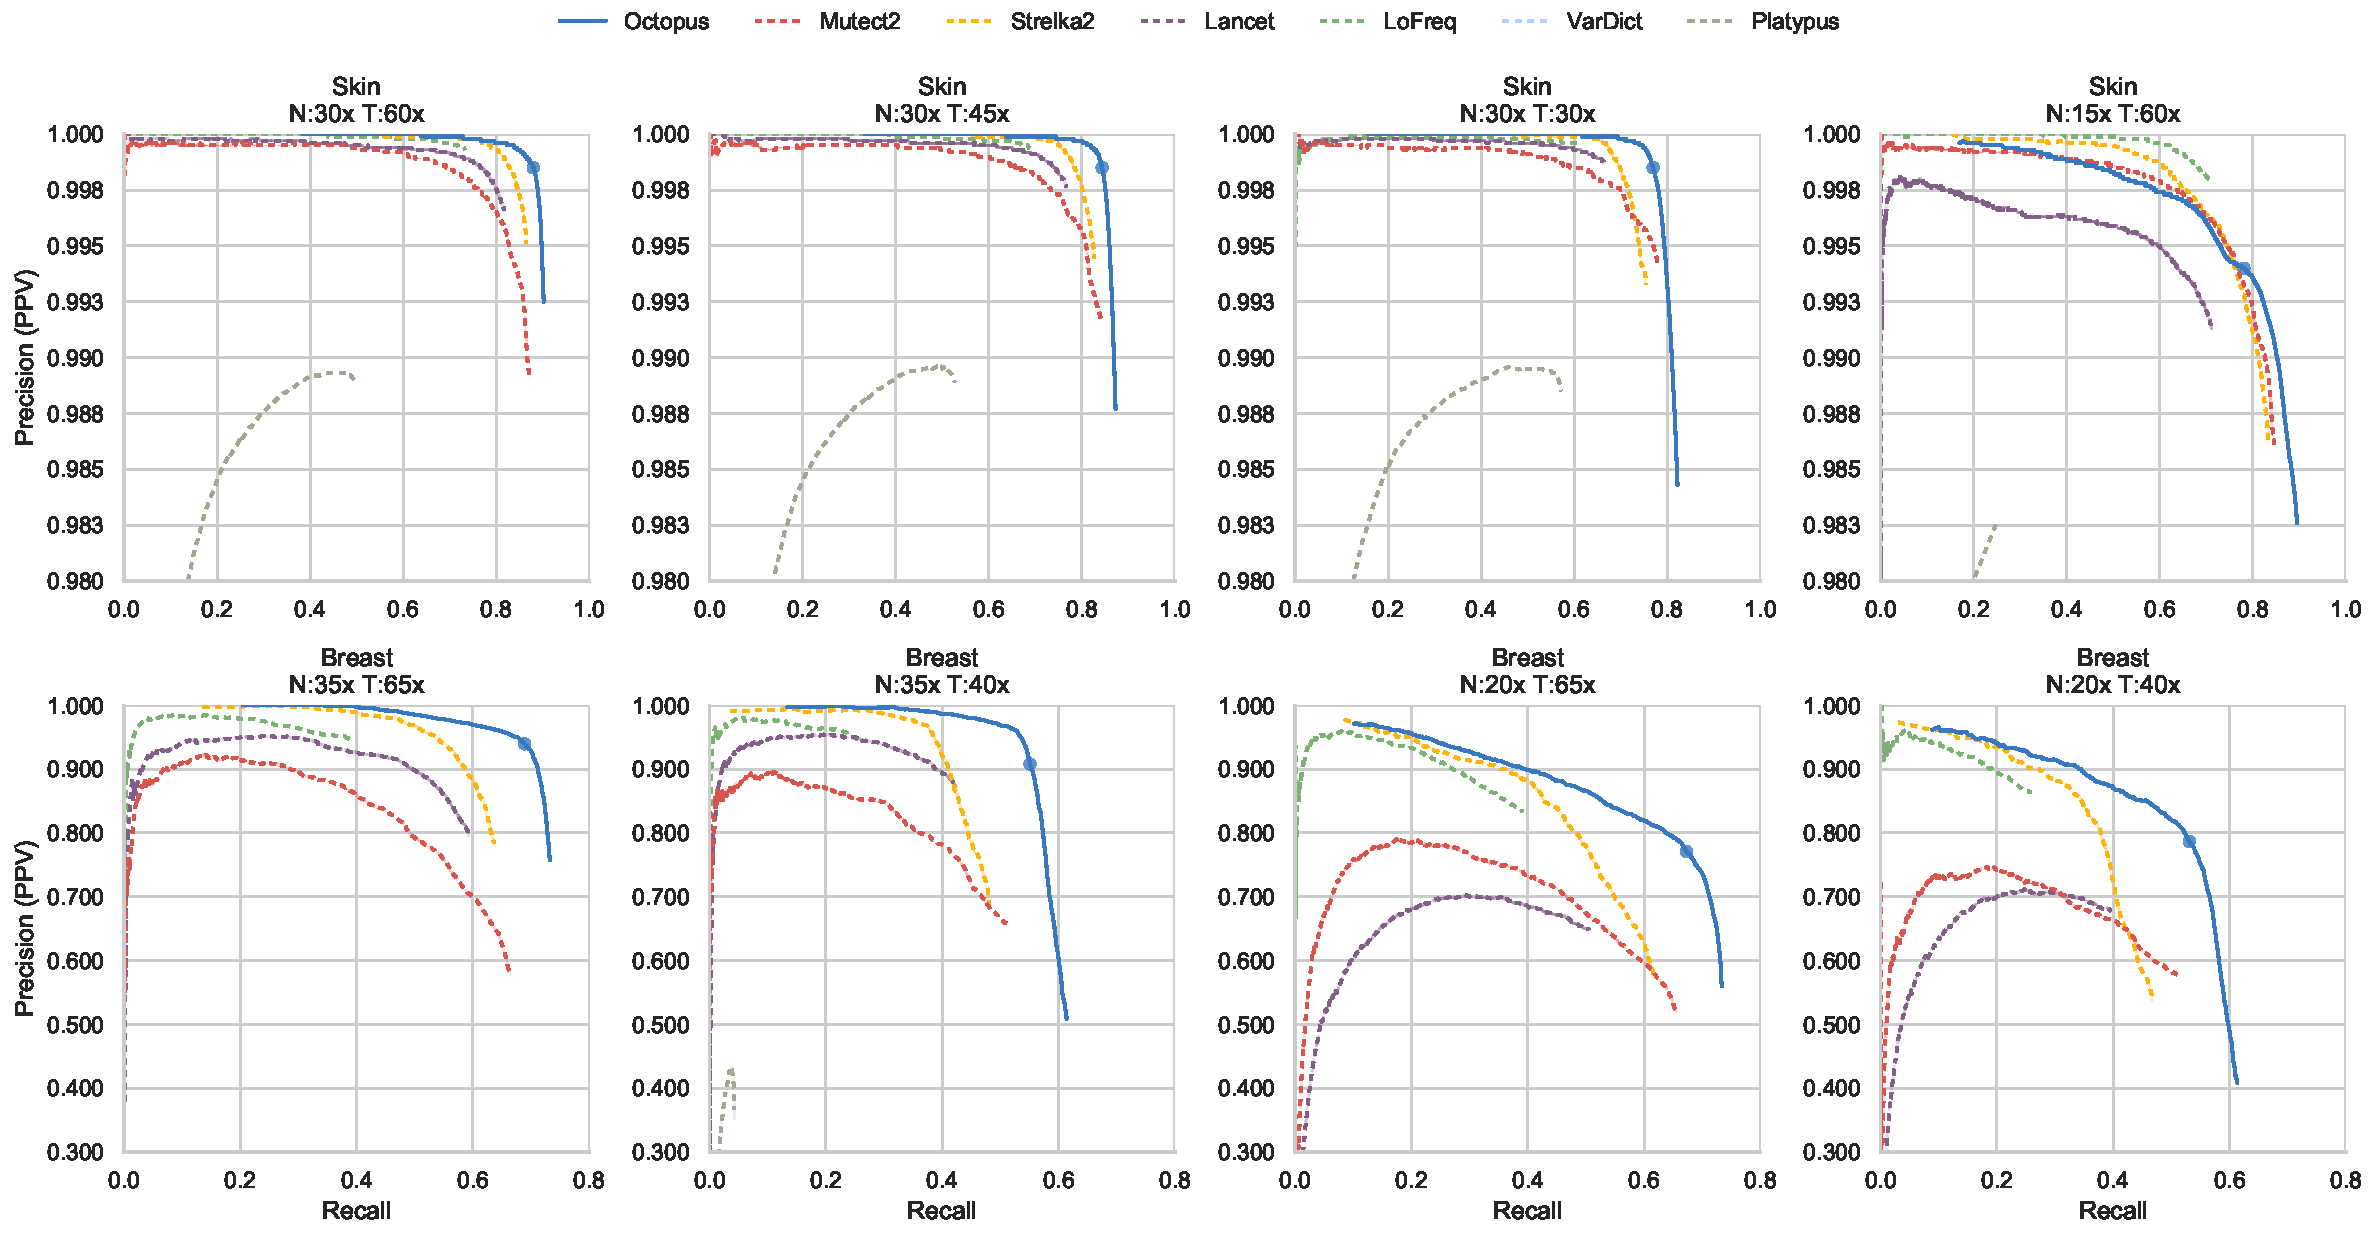
\includegraphics[width=\textwidth]{figures/paired_somatic_precision_recall}
        \caption{}
        \label{supfig:paired-somatic-pr}
    \end{subfigure}
    \begin{subfigure}[b]{\textwidth}
        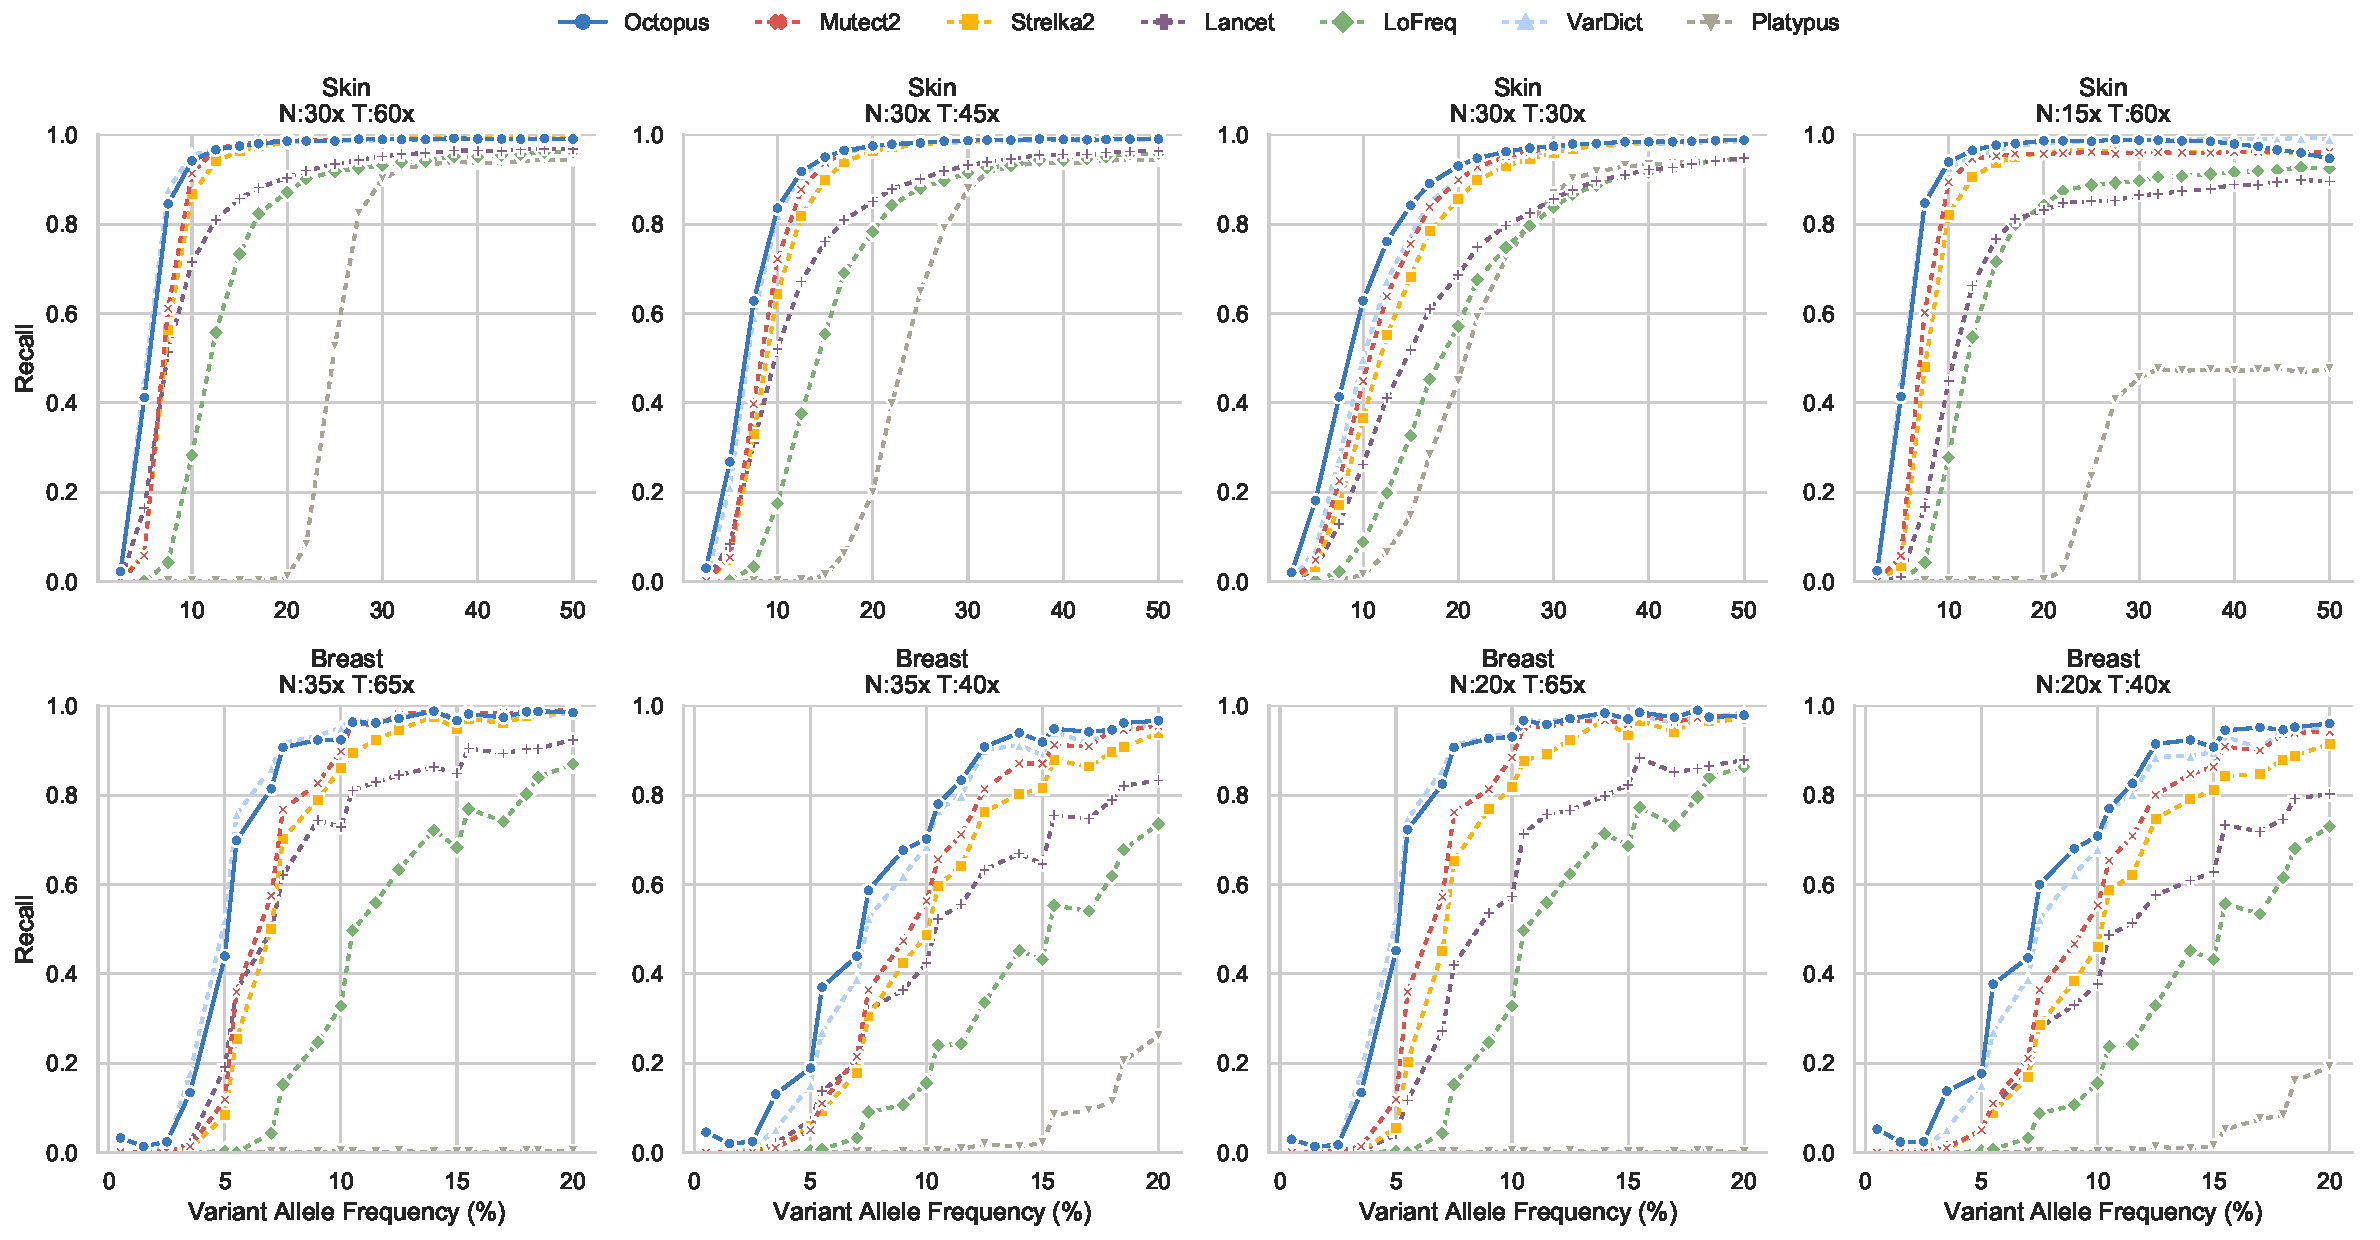
\includegraphics[width=\textwidth]{figures/paired_somatic_vaf_recall}
        \caption{}
        \label{supfig:paired-somatic-vaf-recall}
    \end{subfigure}
    \caption{Somatic mutation calling accuracy for synthetic skin and breast tumours with a paired normal sample with downsampling applied. \textbf{\subref{supfig:paired-somatic-pr}} Precision-recall curves. Scoring metrics used to generate curves were RFQUAL (Octopus), TLOD (Mutect2), SomaticEVS (Strelka2), QUAL (Lancet), QUAL (LoFreq), SSF (VarDict), and QUAL (Platypus). Only PASS calls are used. VarDict is not visible as it is outside the axis limits due to low precision. Precisions on the two tests are substantially different as the skin set has almost $50$ times as many true mutations as the breast set. Dots on the Octopus curve are placed at RFQUAL 7 (3 is used for the entire curve). \textbf{\subref{supfig:paired-somatic-vaf-recall}} Recalls for each Variant Allele Frequency (VAF) using PASS variants. Points show true spike-in VAFs. All comparisons to the synthetic tumour truth sets were performed using RTG Tools vcfeval (version 3.9.1).} 
    \label{supfig:synthetic-tumours}
\end{figure*}

\clearpage

\begin{figure}[ht!]
    \centering
    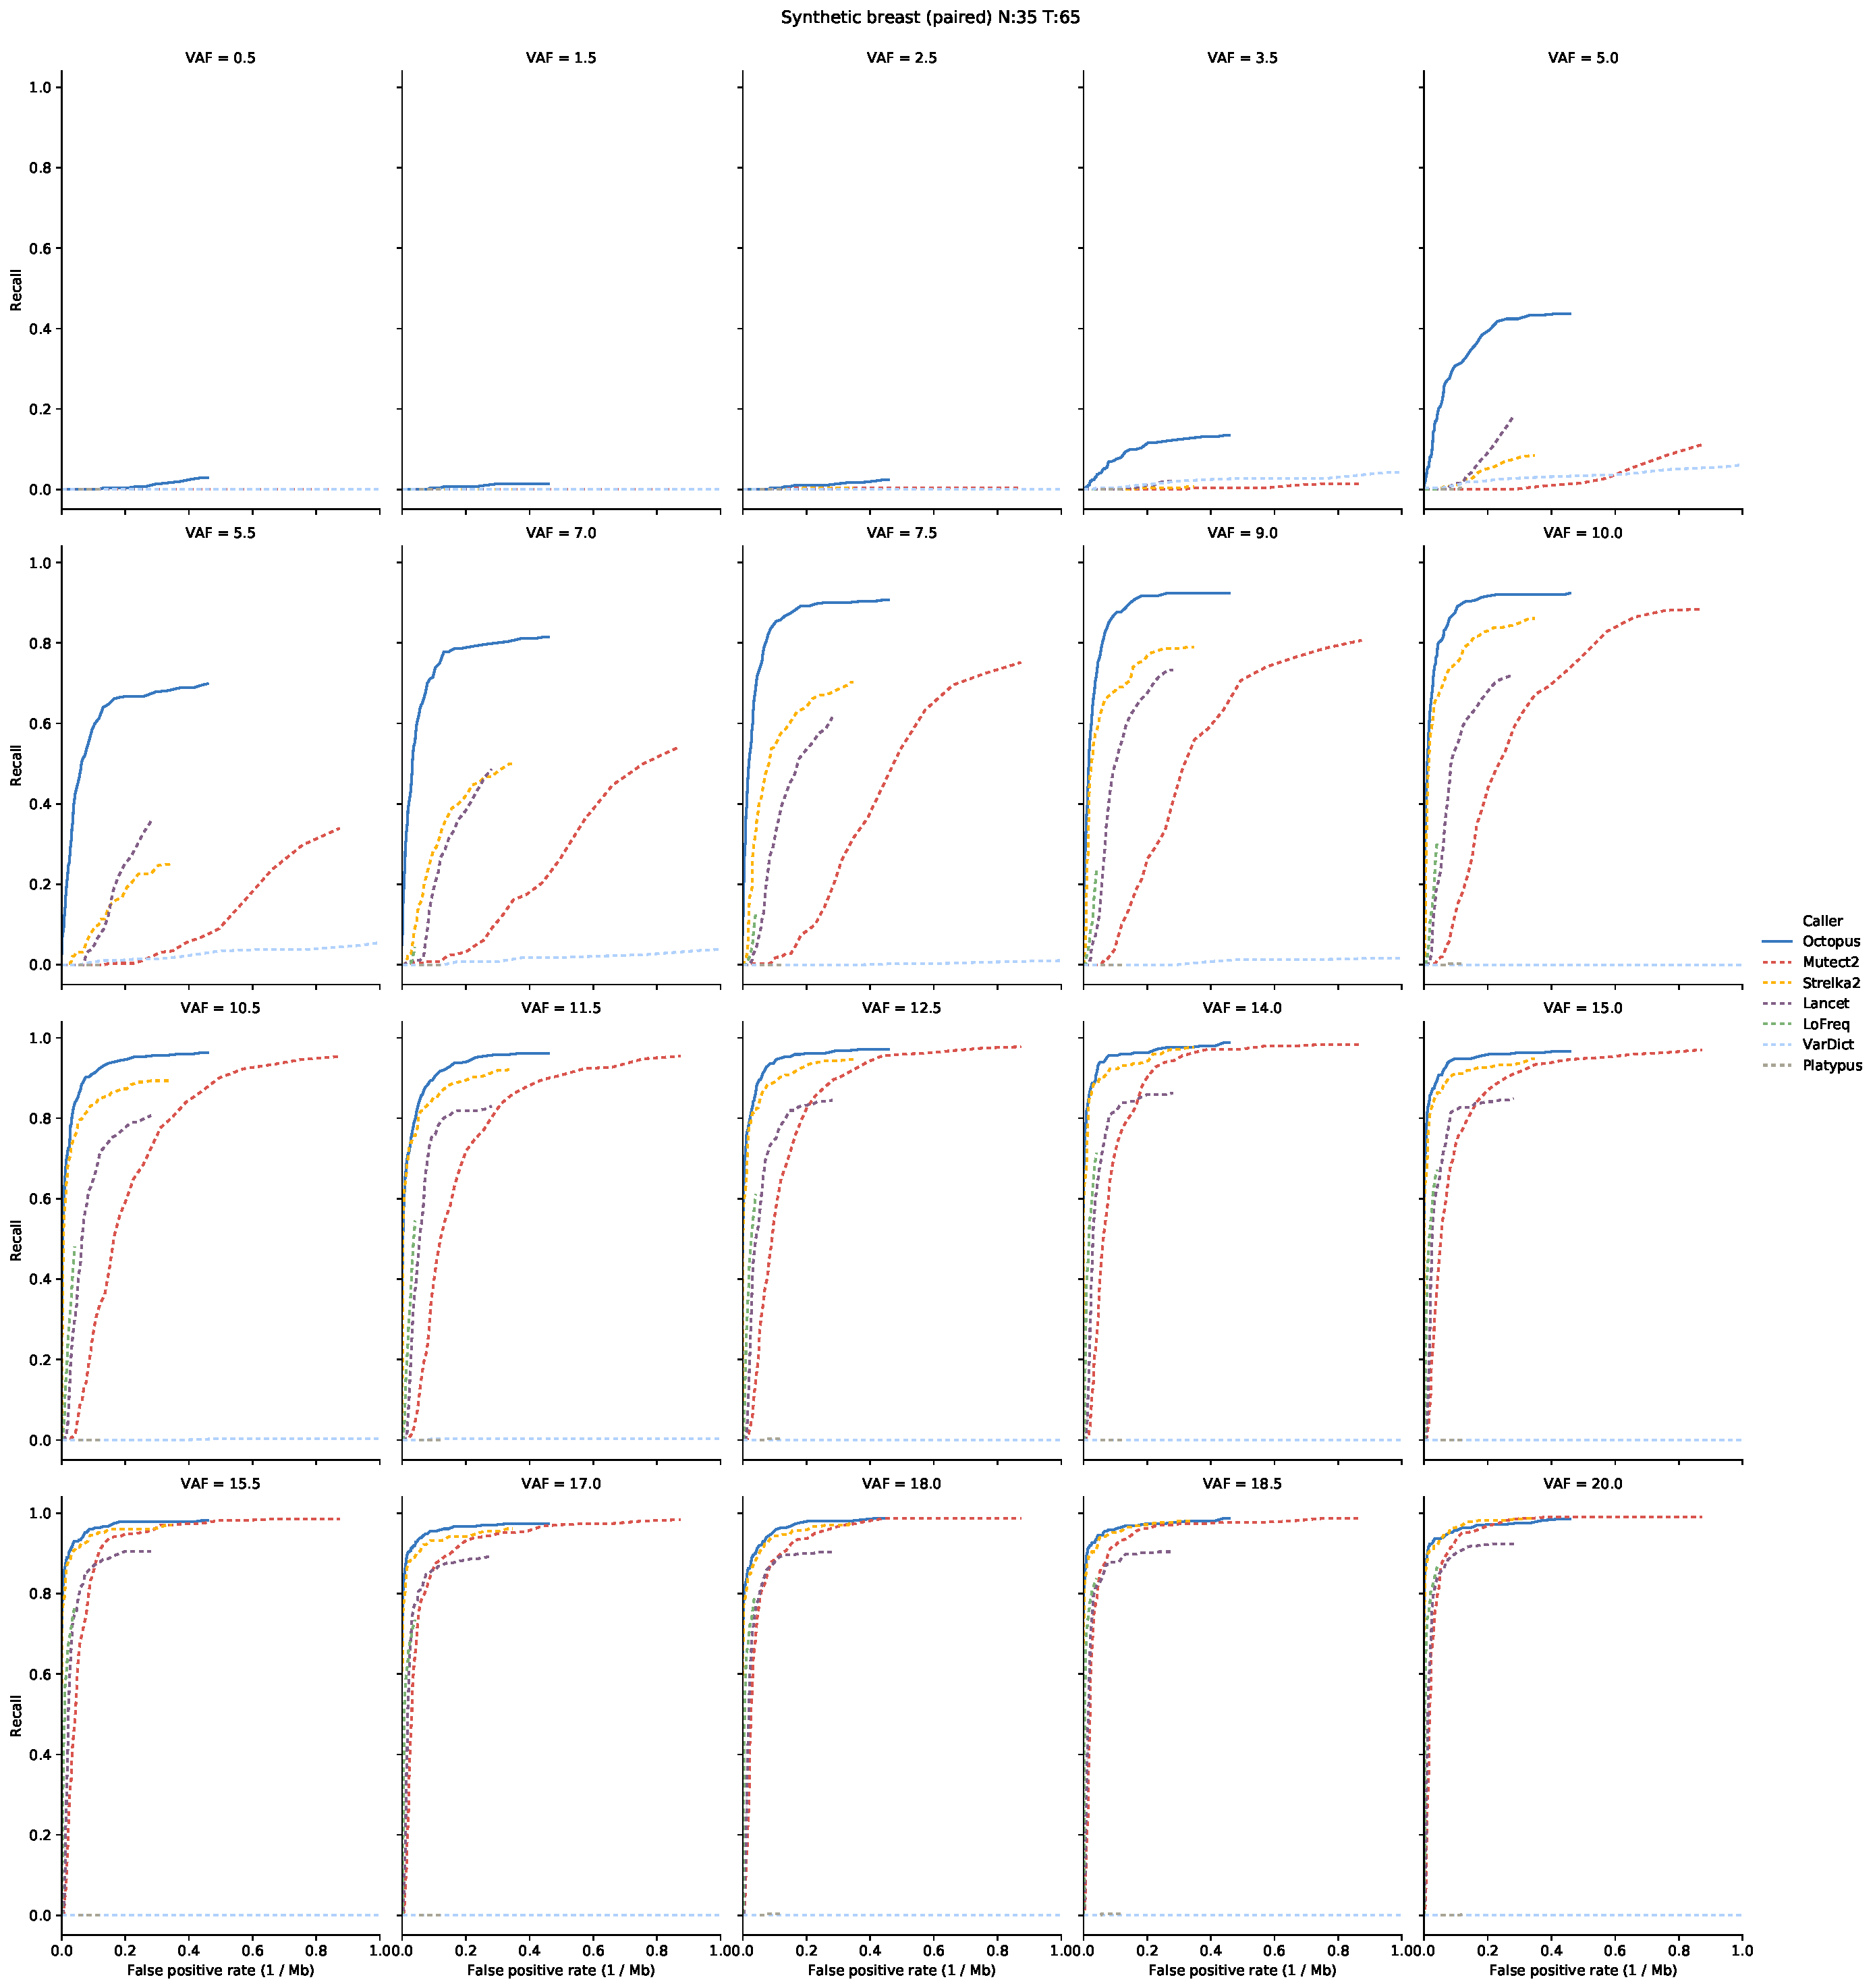
\includegraphics[width=\textwidth]{figures/paired_somatic_breast_n35_t65_vaf_recall.pdf}
    \caption{Evaluation of VAF sensitivity in paired synthetic breast sample. Scoring metrics used to generate curves were RFQUAL (Octopus), TLOD (Mutect2), SomaticEVS (Strelka2), QUAL (Lancet), QUAL (LoFreq), SSF (VarDict), and QUAL (Platypus). The false positive rate were calculated using all false positive calls at each score threshold. Calls were compared to the truth sets using RTG Tools vcfeval.}
    \label{supfig:paired-somatic-breast-n35-t65-vaf}
\end{figure}

\clearpage

\begin{figure}[ht!]
    \centering
    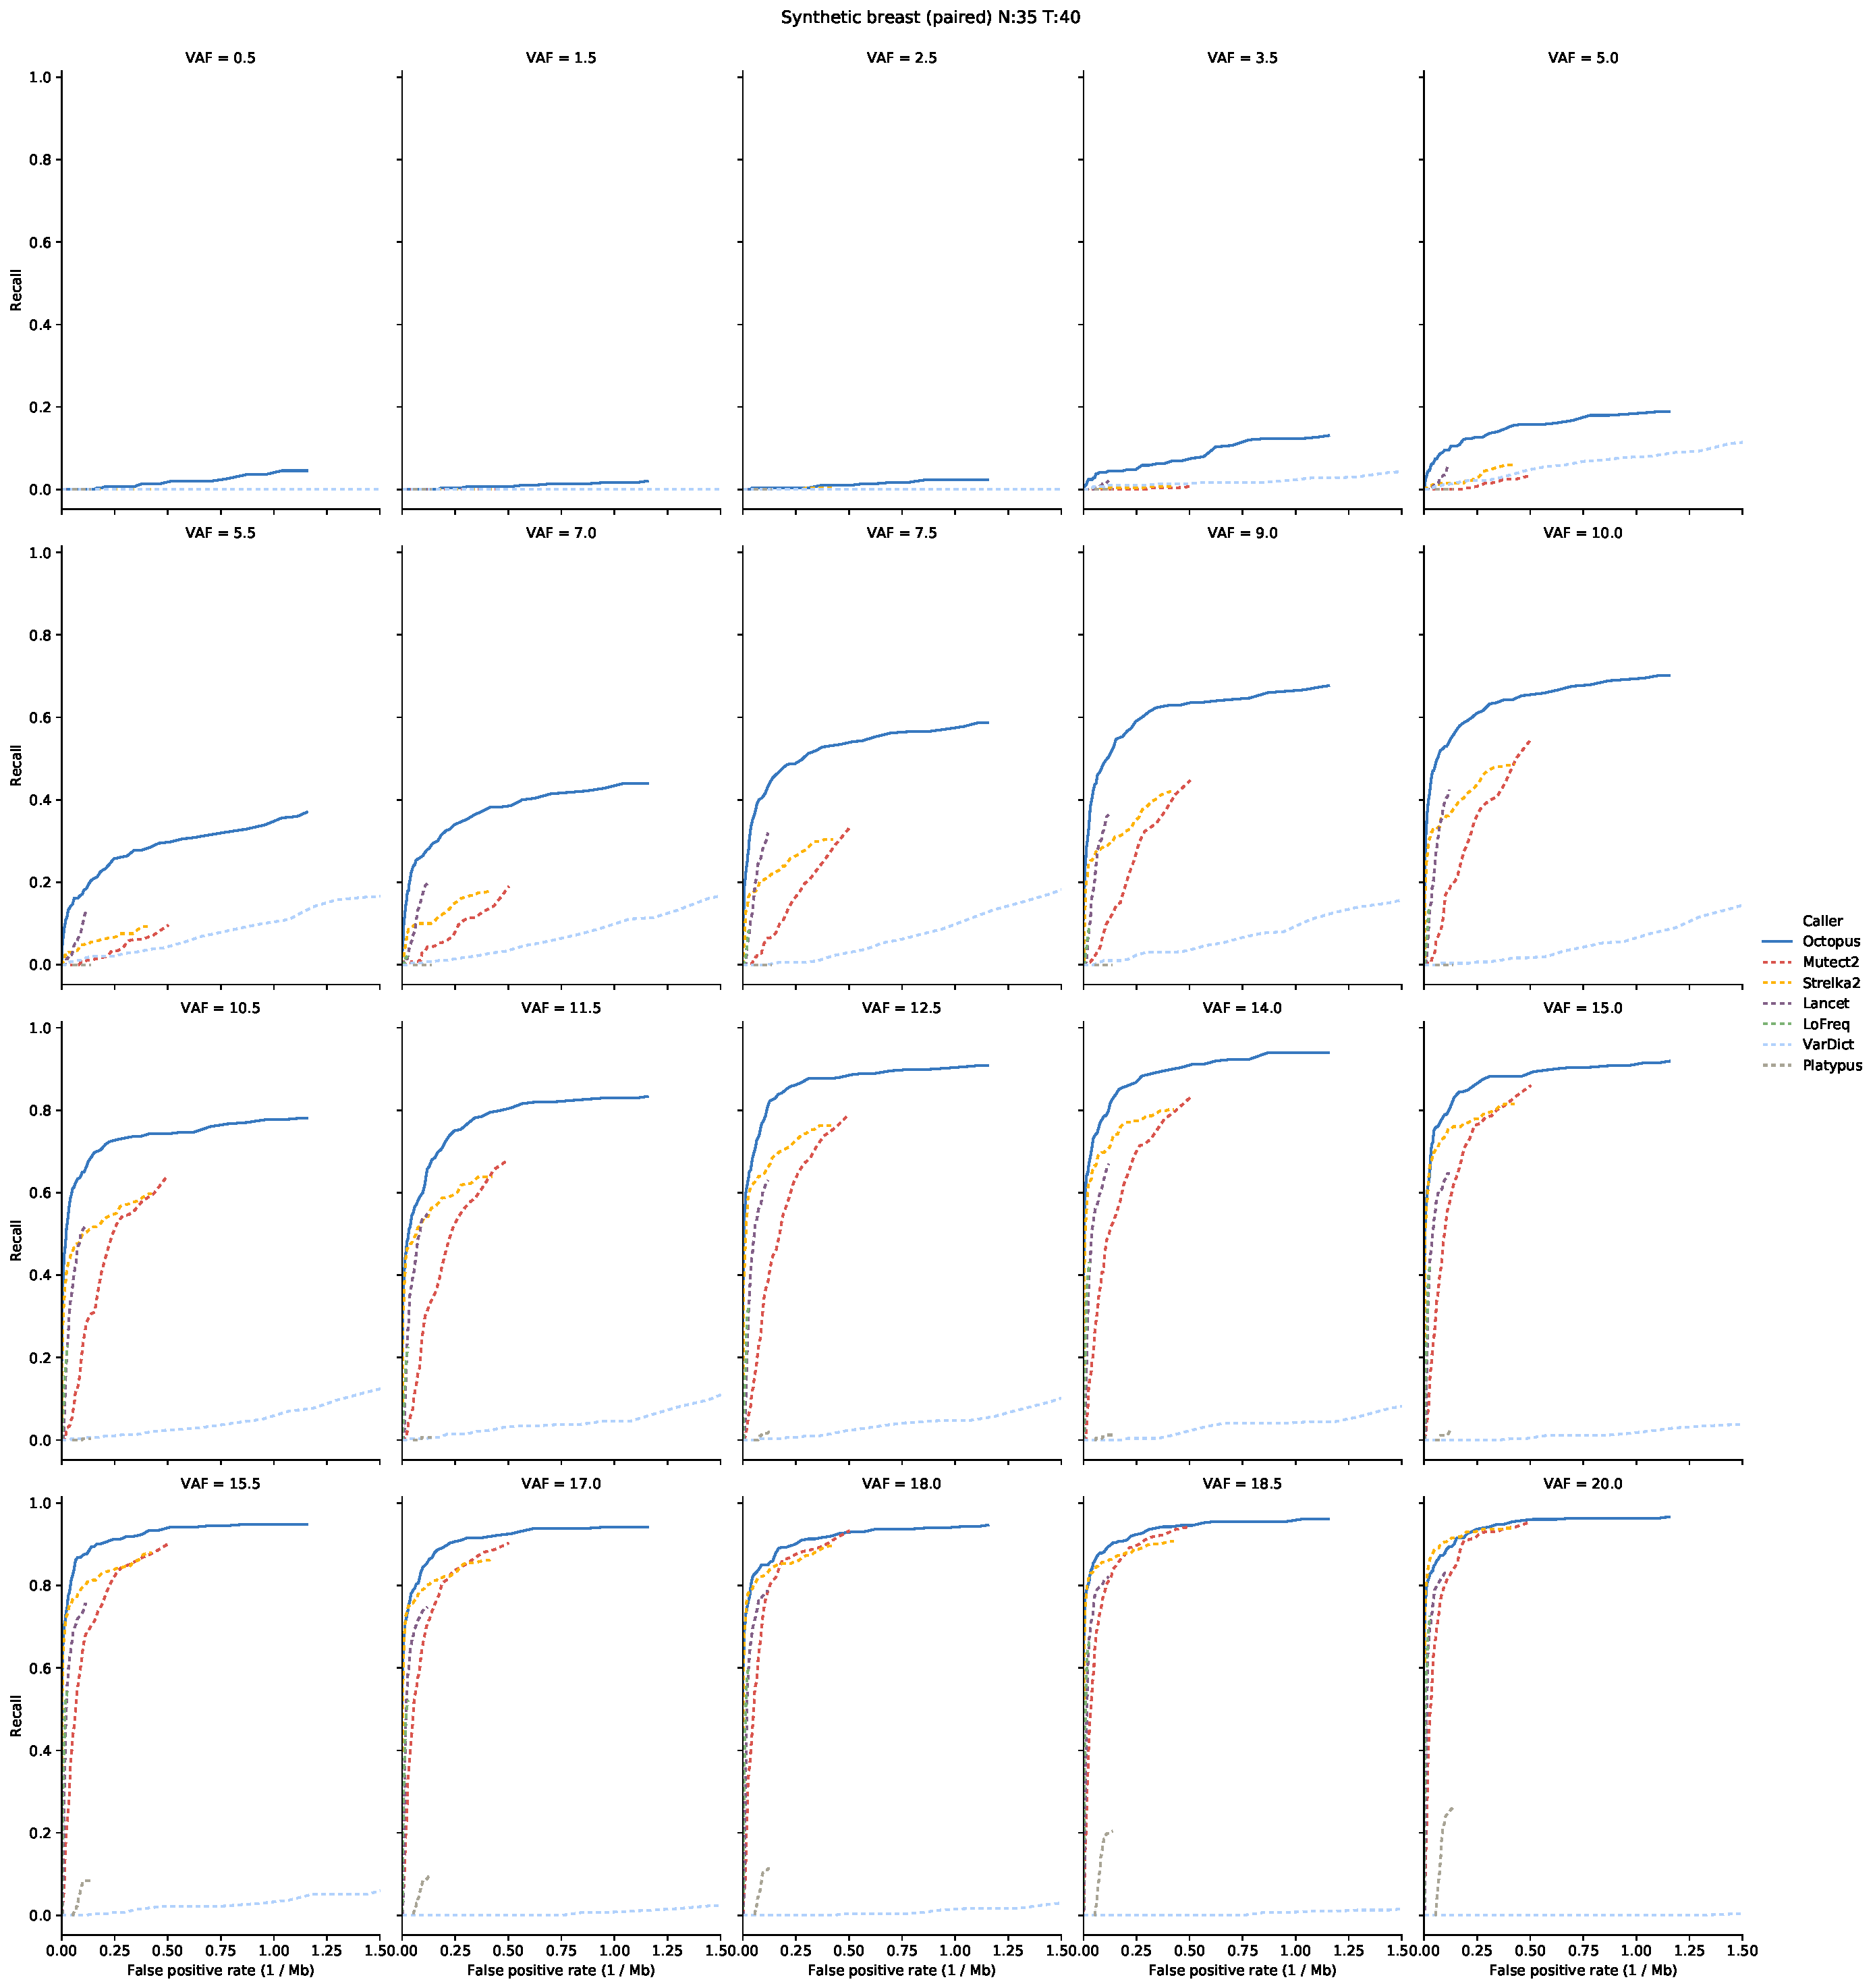
\includegraphics[width=\textwidth]{figures/paired_somatic_breast_n35_t40_vaf_recall.pdf}
    \caption{Evaluation of VAF sensitivity in paired synthetic breast sample with downsampled tumour sample. Scoring metrics used to generate curves were RFQUAL (Octopus), TLOD (Mutect2), SomaticEVS (Strelka2), QUAL (Lancet), QUAL (LoFreq), SSF (VarDict), and QUAL (Platypus). The false positive rate were calculated using all false positive calls at each score threshold. Calls were compared to the truth sets using RTG Tools vcfeval.}
    \label{supfig:paired-somatic-breast-n35-t40-vaf}
\end{figure}

\clearpage

\begin{figure}[ht!]
    \centering
    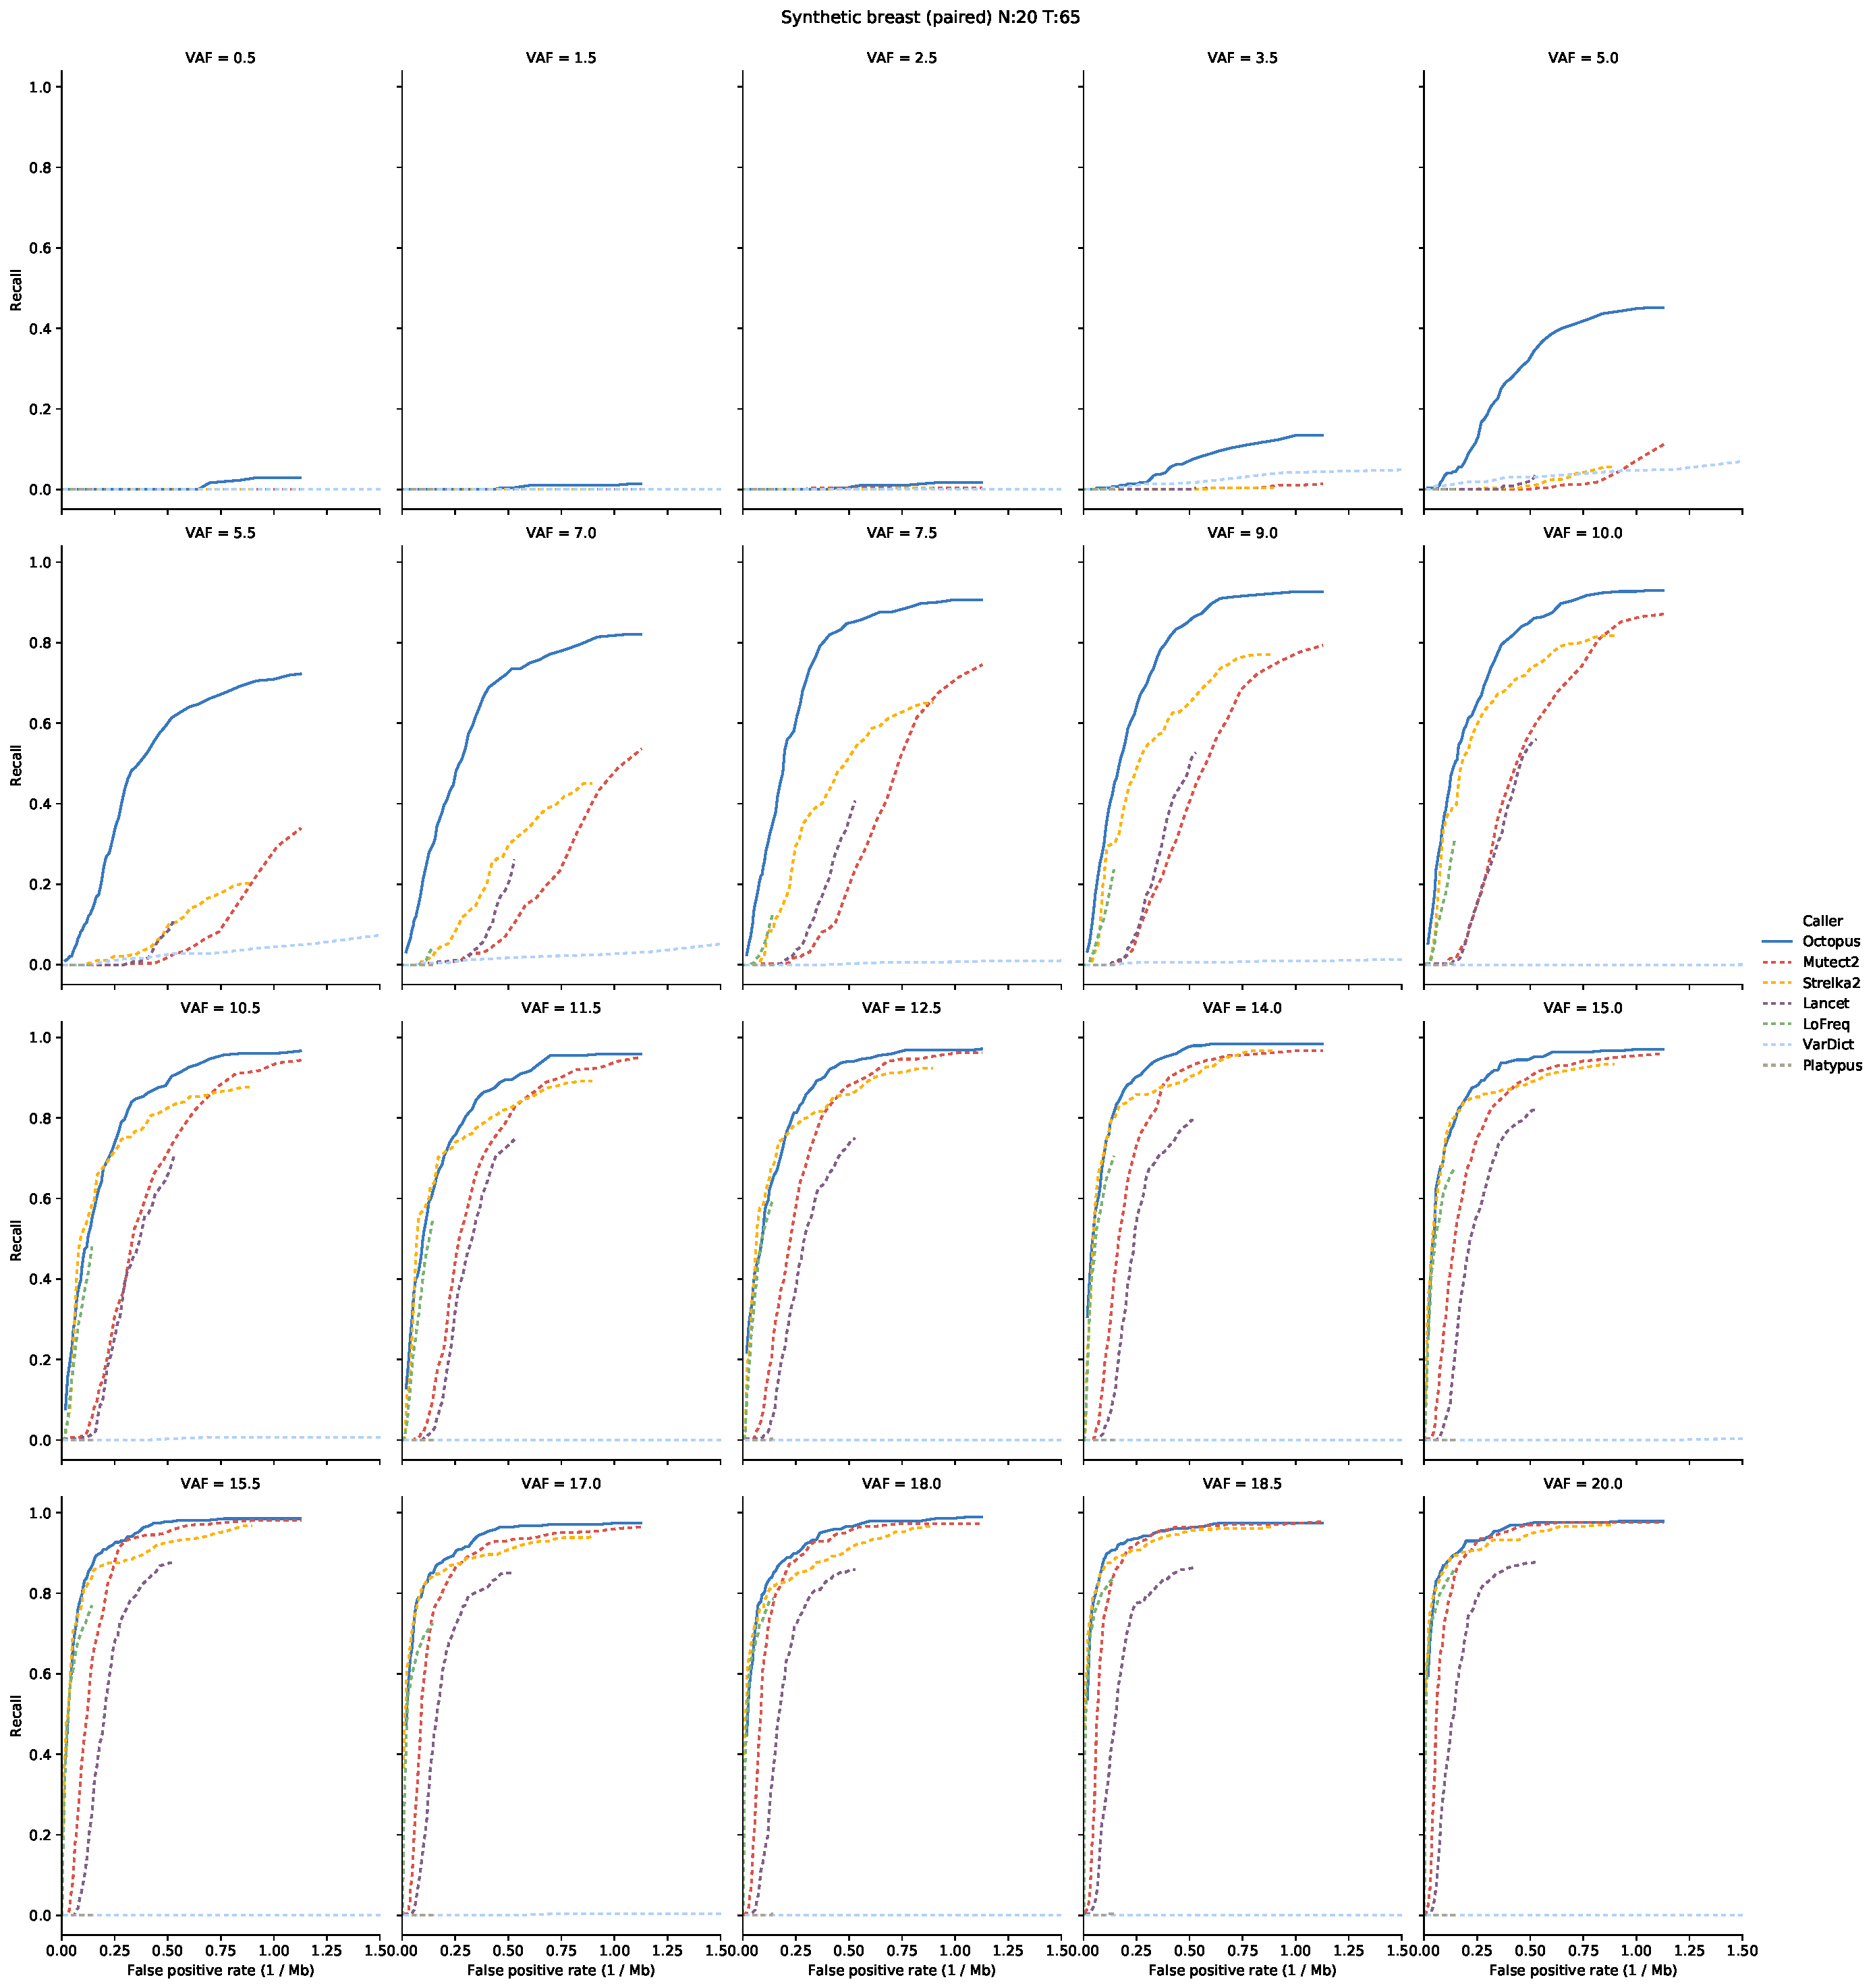
\includegraphics[width=\textwidth]{figures/paired_somatic_breast_n20_t65_vaf_recall.pdf}
    \caption{Evaluation of VAF sensitivity in paired synthetic breast sample with downsampled normal sample. Scoring metrics used to generate curves were RFQUAL (Octopus), TLOD (Mutect2), SomaticEVS (Strelka2), QUAL (Lancet), QUAL (LoFreq), SSF (VarDict), and QUAL (Platypus). The false positive rate were calculated using all false positive calls at each score threshold. Calls were compared to the truth sets using RTG Tools vcfeval.}
    \label{supfig:paired-somatic-breast-n20-t65-vaf}
\end{figure}

\clearpage

\begin{figure}[ht!]
    \centering
    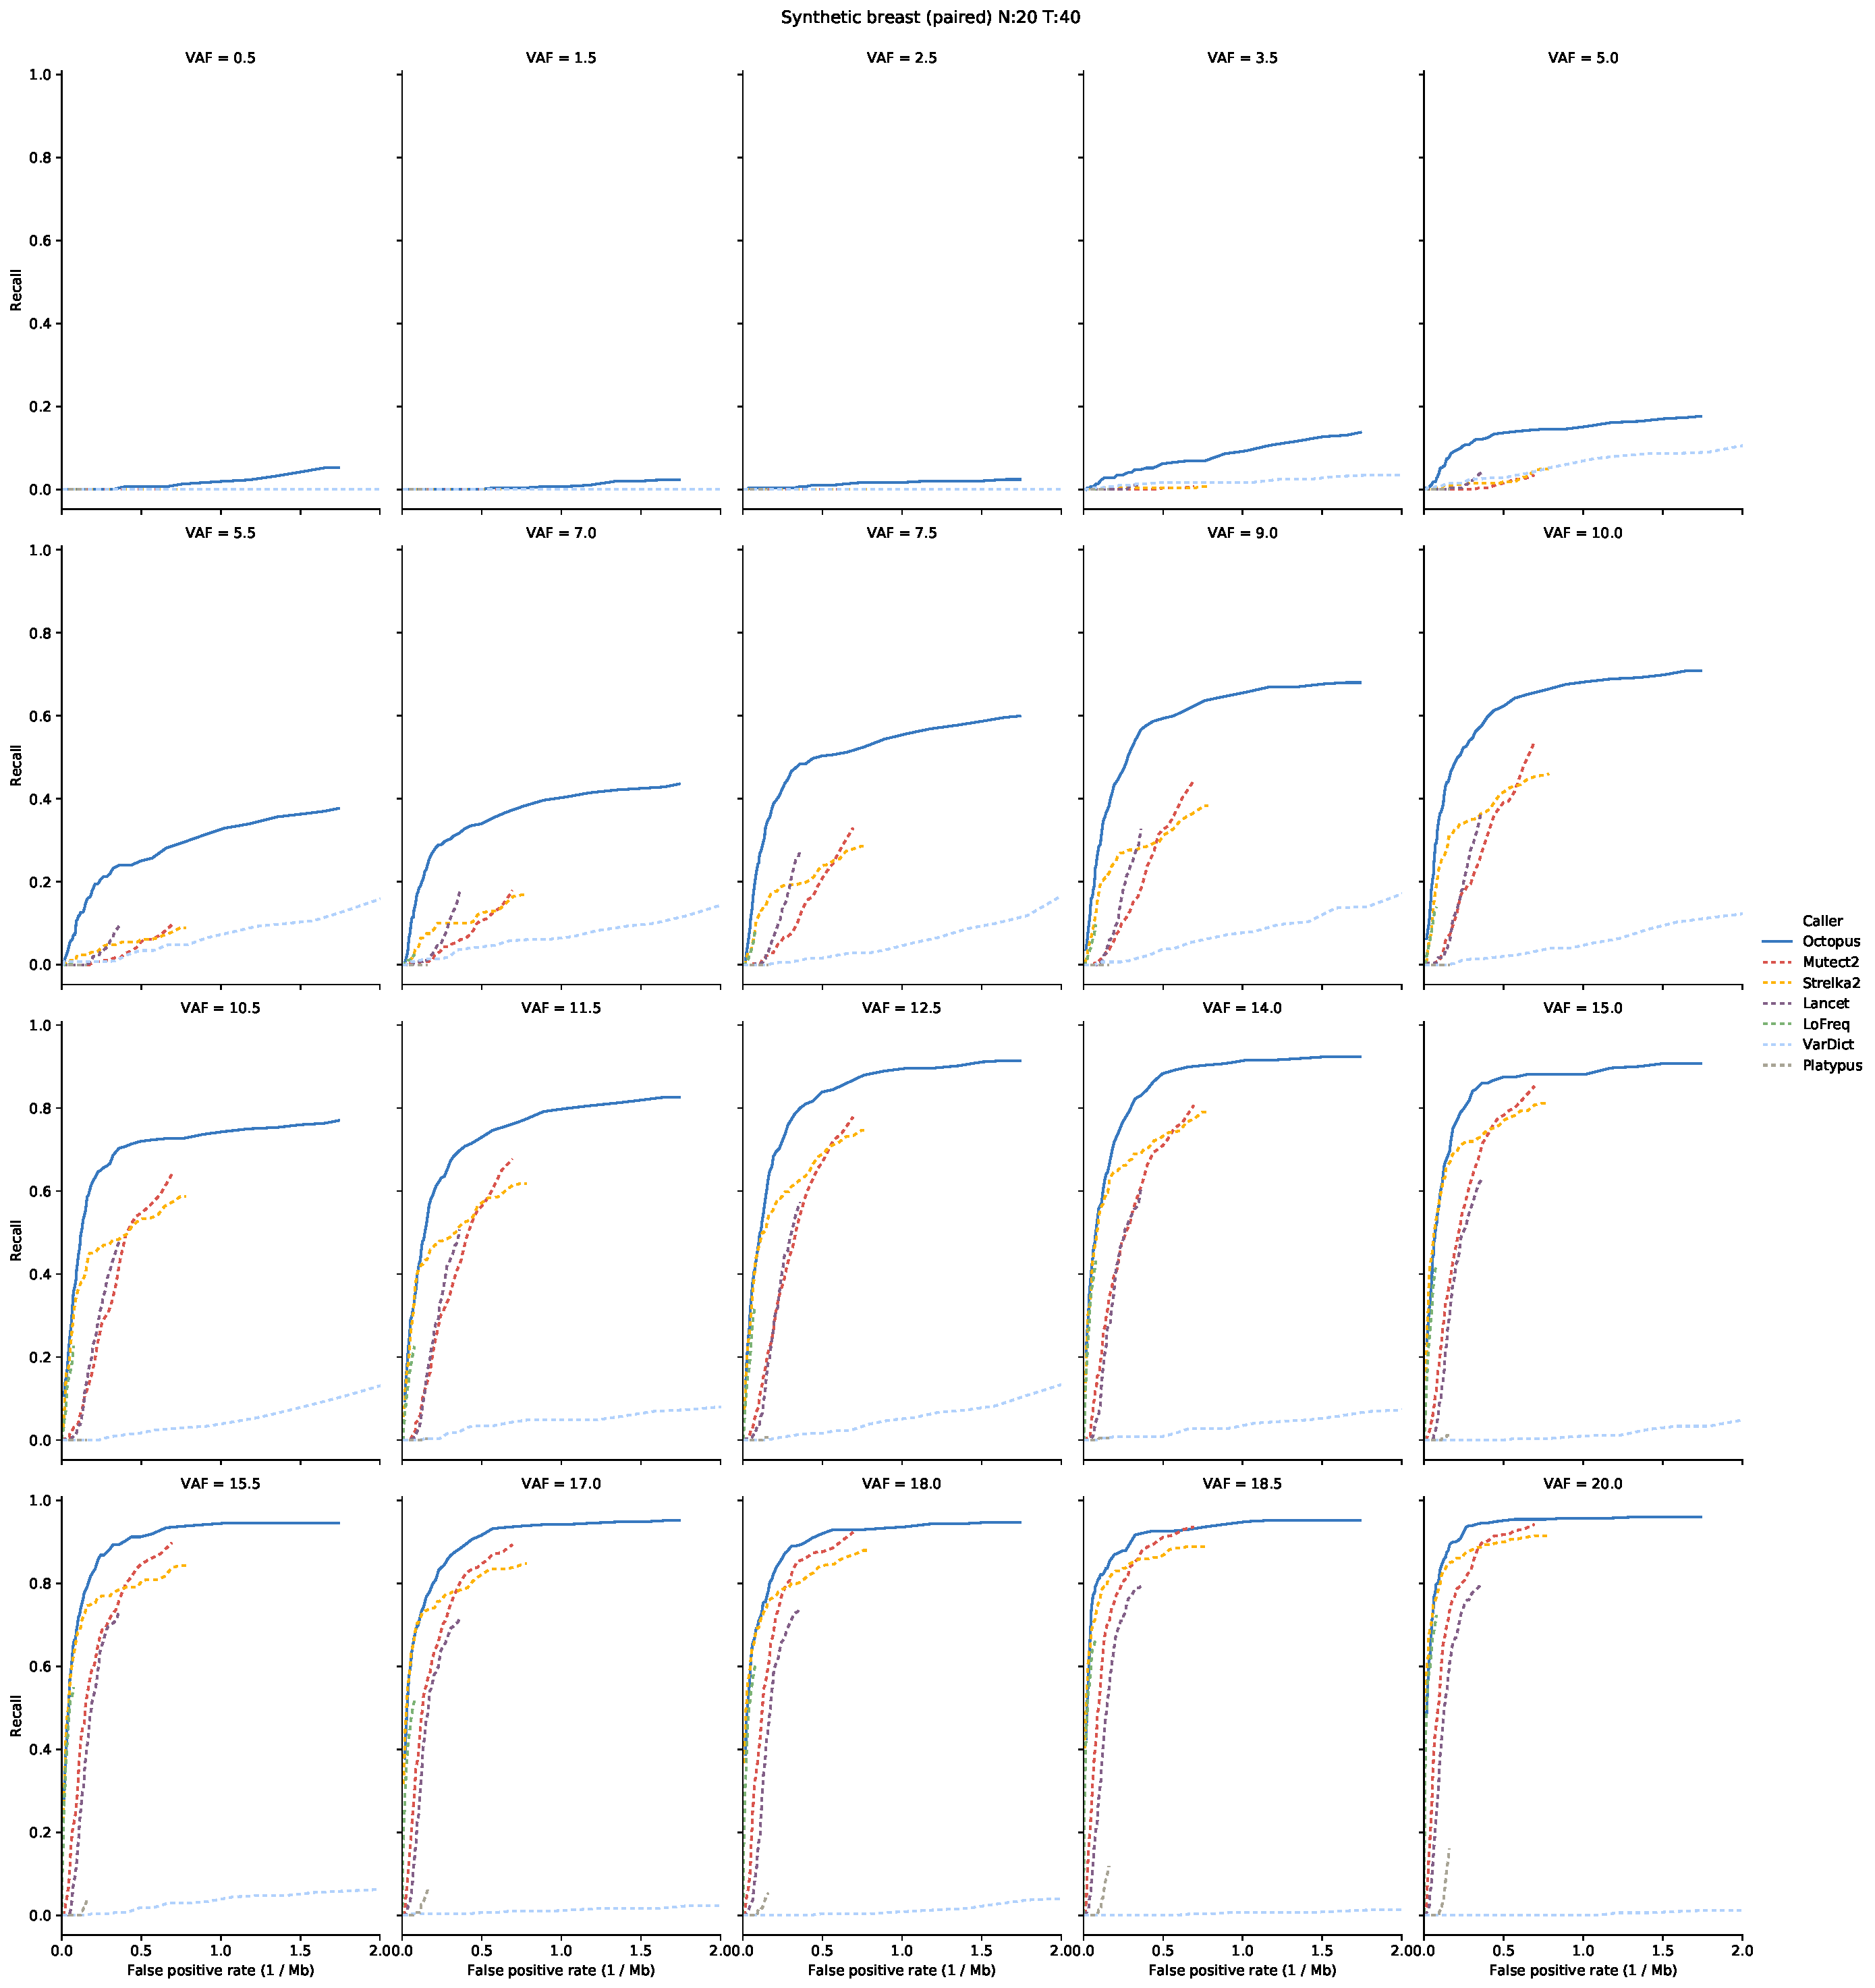
\includegraphics[width=\textwidth]{figures/paired_somatic_breast_n20_t40_vaf_recall.pdf}
    \caption{Evaluation of VAF sensitivity in paired synthetic breast sample with downsampled normal and normal samples. Scoring metrics used to generate curves were RFQUAL (Octopus), TLOD (Mutect2), SomaticEVS (Strelka2), QUAL (Lancet), QUAL (LoFreq), SSF (VarDict), and QUAL (Platypus). The false positive rate were calculated using all false positive calls at each score threshold. Calls were compared to the truth sets using RTG Tools vcfeval.}
    \label{supfig:paired-somatic-breast-n20-t40-vaf}
\end{figure}

\clearpage

\begin{table}[ht!]
    \centering
    \caption{Unpaired somatic benchmarks summary.}
    \label{suptable:unpaired-somatic}
    \small
    \sffamily
    \resizebox{\linewidth}{!}{%
    \begin{tabular}{llllllllll}
    \toprule
       Tumour &   Caller &         Test & True-pos-baseline & True-pos-call & False-pos & False-neg & Precision & Sensitivity & F-measure \\
    \midrule
   skin &  Octopus &       combined &           3748037 &       3770554 &     11129 &     90523 &    0.9971 &      0.9764 &    0.9866 \\
   skin &  Octopus &        somatic &            153332 &        153332 &     10740 &    108579 &    0.9345 &      0.5854 &    0.7199 \\
   skin &   Pisces &       combined &           3711460 &       3718366 &    112203 &    127088 &    0.9707 &      0.9669 &    0.9688 \\
   skin &   Pisces &        somatic &             65242 &         65242 &     71600 &    196669 &    0.4768 &      0.2491 &    0.3272 \\
 breast &  Octopus &       combined &           3624884 &       3648238 &     11566 &     71775 &    0.9968 &      0.9806 &    0.9886 \\
 breast &  Octopus &        somatic &              3978 &          3978 &      9948 &      1527 &    0.2857 &      0.7226 &    0.4094 \\
 breast &   Pisces &       combined &           3607097 &       3614212 &    124363 &     89555 &    0.9667 &      0.9758 &    0.9712 \\
 breast &   Pisces &        somatic &              3115 &          3115 &     84648 &      2390 &    0.0355 &      0.5658 &    0.0668 \\
    \bottomrule
    \end{tabular}
    }
\end{table}

\clearpage

\begin{figure}[ht!]
    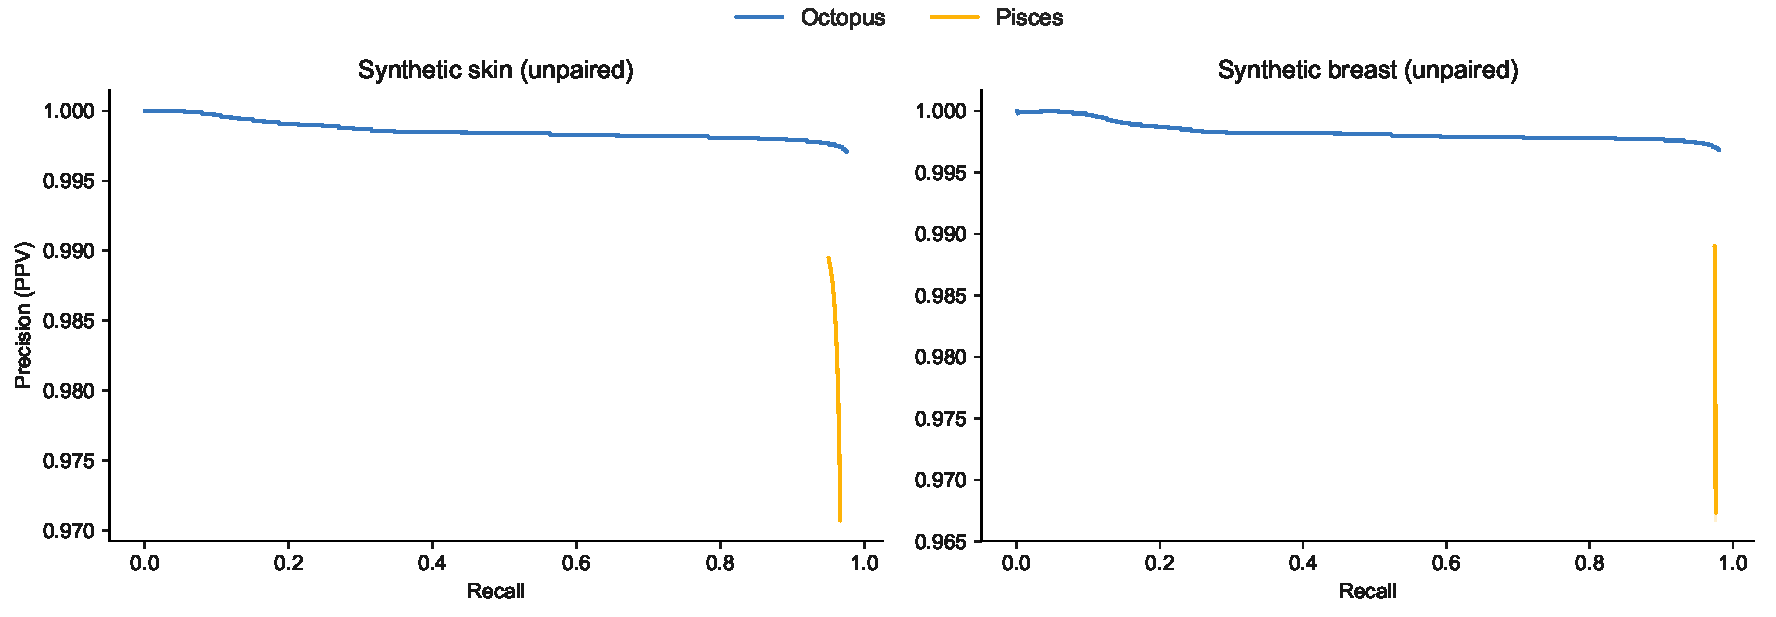
\includegraphics[width=\textwidth]{figures/tumour-only-combined-precision-recalls}
    \caption{Tumour-only combined germline and somatic precision-recall.}
    \label{supfig:filtering}
\end{figure}

\clearpage

\begin{figure}[ht!]
    \centering
    \begin{subfigure}[b]{0.31\textwidth}
        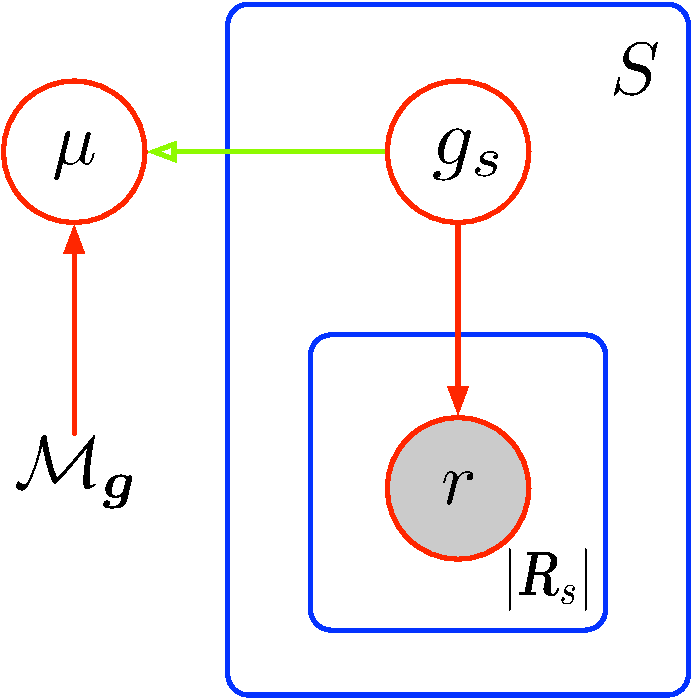
\includegraphics[width=\textwidth]{figures/population_model}
        \caption{}
        \label{supfig:pop}
    \end{subfigure}
    \hfill
    \begin{subfigure}[b]{0.31\textwidth}
        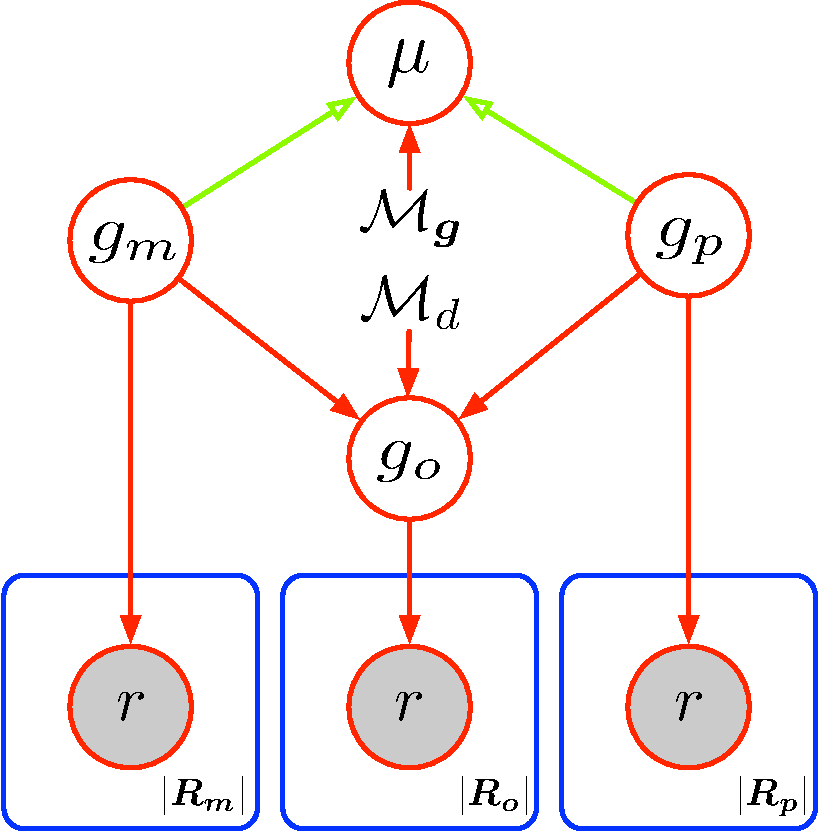
\includegraphics[width=\textwidth]{figures/trio_model}
        \caption{}
        \label{supfig:trio}
    \end{subfigure}
    \hfill
    \begin{subfigure}[b]{0.31\textwidth}
        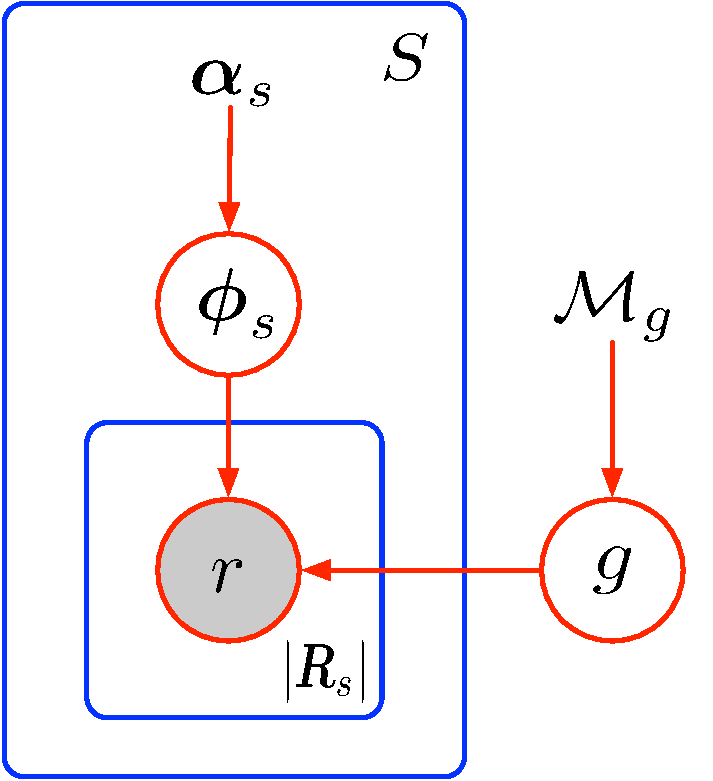
\includegraphics[width=\textwidth]{figures/subclone_model}
        \caption{}
        \label{supfig:subclone}
    \end{subfigure}
    \caption{Genotype models shown in plate notation. \textbf{\subref{supfig:pop}} Population. \textbf{\subref{supfig:trio}} Trio. \textbf{\subref{supfig:subclone}} Subclone. Symbols insides circles are latent variables, observed variables are shaded. Symbols inside boxes are repeated. Symbols not inside a circle are parameters or models. Arrows define conditional relationships, red for stochastic and green for deterministic. $\mu$ is used to denote parameters for a joint genotype prior model $\mathcal{M}_g$. Remaining symbols are defined in the the Online Methods.}
    \label{fig:genotype-models}
\end{figure}

\clearpage

\section*{Supplementary Note 1. Data and software}

\subsection*{Software versions}

\subsubsection*{General}

\begin{itemize}
    \item BWA (0.7.17-r1188)
    \item Samtools (1.7)
    \item Bcftools (1.7)
    \item RTG Tools (3.9.1)
\end{itemize}

\subsubsection*{Germline and \textit{de novo} analysis}

\begin{itemize}
    \item Octopus (v0.5.2-beta)
    \item DeepVariant (v0.5.1)
    \item GATK4 (v4.0.0.0)
    \item Platypus (0.8.1)
    \item Strelka2 (v2.9.1)
\end{itemize}

\subsubsection*{Somatic analysis}

\begin{itemize}
    \item Octopus (v0.5.1-beta)
    \item Mutect2 (GATK4 v4.0.0.0)
    \item Platypus (0.8.1)
    \item Strelka2 (v2.9.1)
    \item LoFreq (v2.1.3.1)
    \item VarDict (1.5.2-java)
    \item Lancet (v1.0.6)
    \item Pisces (5.2.7.47)
\end{itemize}

\subsection*{Data sources}

\subsubsection*{References}

We used hs37d5 (\url{ftp://ftp-trace.ncbi.nih.gov/1000genomes/ftp/technical/reference/phase2_reference_assembly_sequence/hs37d5.fa.gz}) for all analysis.

\begin{landscape}
\subsubsection*{Germline truth data}

\noindent\begin{tabularx}{\linewidth}{lXX}
    \toprule
       Name &   Truth VCF &   High confidence BED  \\
    \midrule
       GIAB HG001 &  \url{ftp://ftp-trace.ncbi.nlm.nih.gov//giab/ftp/release/NA12878_HG001/NISTv3.3.2/GRCh37/HG001_GRCh37_GIAB_highconf_CG-IllFB-IllGATKHC-Ion-10X-SOLID_CHROM1-X_v.3.3.2_highconf_PGandRTGphasetransfer.vcf.gz}  &   \url{ftp://ftp-trace.ncbi.nlm.nih.gov//giab/ftp/release/NA12878_HG001/NISTv3.3.2/GRCh37/HG001_GRCh37_GIAB_highconf_CG-IllFB-IllGATKHC-Ion-10X-SOLID_CHROM1-X_v.3.3.2_highconf_nosomaticdel.bed}  \\
       GIAB HG002 &  \url{ftp://ftp-trace.ncbi.nlm.nih.gov//giab/ftp/release/AshkenazimTrio/HG002_NA24385_son/NISTv3.3.2/GRCh37/HG002_GRCh37_GIAB_highconf_CG-IllFB-IllGATKHC-Ion-10X-SOLID_CHROM1-22_v.3.3.2_highconf_triophased.vcf.gz}  &   \url{ftp://ftp-trace.ncbi.nlm.nih.gov//giab/ftp/release/AshkenazimTrio/HG002_NA24385_son/NISTv3.3.2/GRCh37/HG002_GRCh37_GIAB_highconf_CG-IllFB-IllGATKHC-Ion-10X-SOLID_CHROM1-22_v.3.3.2_highconf_noinconsistent.bed}  \\
       GIAB HG005 &  \url{ftp://ftp-trace.ncbi.nlm.nih.gov//giab/ftp/release/ChineseTrio/HG005_NA24631_son/NISTv3.3.2/GRCh37/HG005_GRCh37_highconf_CG-IllFB-IllGATKHC-Ion-SOLID_CHROM1-22_v.3.3.2_highconf.vcf.gz}  &   \url{ftp://ftp-trace.ncbi.nlm.nih.gov//giab/ftp/release/ChineseTrio/HG005_NA24631_son/NISTv3.3.2/GRCh37/HG005_GRCh37_highconf_CG-IllFB-IllGATKHC-Ion-SOLID_CHROM1-22_v.3.3.2_highconf_noMetaSV.bed}  \\
    CHM1-CHM13 & \url{https://github.com/lh3/CHM-eval/releases/download/v0.5/CHM-evalkit-20180222.tar} (full.37m.vcf.gz)  & \url{https://github.com/lh3/CHM-eval/releases/download/v0.5/CHM-evalkit-20180222.tar} (full.37m.bed.gz)  \\
    \bottomrule
\end{tabularx}
\end{landscape}
\newpage

\begin{landscape}
\subsubsection*{Germline analysis sequencing data}

\noindent\begin{tabularx}{\linewidth}{llXl}
    \toprule
       Name & BAM/FASTQ &   URL(s) & Notes  \\
    \midrule
    Precision FDA Truth (HG001) & FASTQ & \url{https://precision.fda.gov/challenges/truth} & Login required to access data \\
    Precision FDA Truth (HG002) & FASTQ & \url{https://precision.fda.gov/challenges/truth} & Login required to access data \\
    Precision FDA Consistency (HG001) & FASTQ & \url{https://precision.fda.gov/challenges/truth} & Login required to access data \\
    GIAB (HG005) & FASTQ & \url{ftp://ftp-trace.ncbi.nlm.nih.gov//giab/ftp/data/ChineseTrio/HG005_NA24631_son/HG005_NA24631_son_HiSeq_300x/basespace_250bps_fastqs/150430_HG005_Homogeneity_03_FCB-22310288} \textbf{and} \url{ftp://ftp-trace.ncbi.nlm.nih.gov//giab/ftp/data/ChineseTrio/HG005_NA24631_son/HG005_NA24631_son_HiSeq_300x/basespace_250bps_fastqs/150506_HG005_Homogeneity_04_FCA-22365346} &  Fastq files were merged. \\
    10X (HG001) & BAM & \url{ftp://ftp-trace.ncbi.nlm.nih.gov//giab/ftp/data/NA12878/10XGenomics/NA12878_phased_possorted_bam.bam} & Mapped to hg19. \\
    10X (HG002) & BAM & \url{ftp://ftp-trace.ncbi.nlm.nih.gov//giab/ftp/data/AshkenazimTrio/HG002_NA24385_son/10XGenomics/NA24385_phased_possorted_bam.bam} & Mapped to hg19. \\
    Platinum Genomes (HG001) & FASTQ &  \url{https://storage.googleapis.com/genomics-public-data/platinum-genomes/fastq/ERR194147_1.fastq.gz} \textbf{and} \url{https://storage.googleapis.com/genomics-public-data/platinum-genomes/fastq/ERR194147_2.fastq.gz} & .\\
    CHM1-CHM13 & BAM & \url{ftp://ftp.sra.ebi.ac.uk/vol1/ERA596/ERA596361/bam/CHM1_CHM13_2.bam} & . \\
    \bottomrule
\end{tabularx}
\end{landscape}
\newpage

\begin{tabular}{llllll}
    \toprule
       Sample &   Library & Library prep & Read Length & Coverage & Instrument  \\
    \midrule
       HG001 &  Truth &       TruSeq DNA PCR-Free &           2x148bp &       ~50x &  HiSeq 2500 \\
       HG001 &  Consistency &       TruSeq Nano DNA Library Prep kit &           2x150bp &       ~40x &  HiSeq X Ten \\
       HG001 &  10X &     10X GemCode  &    2x98bp &       ~34x &  HiSeq 2500 \\
       HG001 &  Platinum &   TruSeq DNA PCR-Free    &    2x101bp &       ~50x &  HiSeq 2000 \\
       HG002 &  Truth &       TruSeq DNA PCR-Free &           2x148bp &       ~50x &  HiSeq 2500 \\
       HG002 &  10X  &     10X GemCode   &   2x98bp &       ~25x &  HiSeq 2500 \\
       HG005 &  GIAB  &     TruSeq DNA PCR-Free   &   2x250bp &       ~50x &  HiSeq 2500 \\
       Syndip &  Broad  &     Kapa Biosystems DNA PCR-Free   &   2x151bp &       ~45x &  HiSeq X Ten \\
    \bottomrule
    \end{tabular}

\subsubsection*{\textit{De novo} analysis sequencing data}

Fastq files for each sample in the trio were obtained from the Wellcome Centre for Human Genetics.

\subsubsection*{Somatic analysis sequencing data}

Fastq files were downloaded from \url{ftp://ftp-trace.ncbi.nlm.nih.gov//giab/ftp/data/NA12878/NIST_NA12878_HG001_HiSeq_300x}.

\subsection*{Germline random forest training data}

For the germline analysis, we used three whole-genome replicates of NA12878 (HG001) for training the random forest:

\begin{enumerate}
    \item High coverage Illumina reads from the 1000G phase 3 project, Aligned reads were downloaded from \url{ftp.1000genomes.ebi.ac.uk:/vol1/ftp/phase3/data/NA12878/high_coverage_alignment/NA12878.mapped.ILLUMINA.bwa.CEU.high_coverage_pcr_free.20130906.bam}.
    \item Low coverage Illumina reads from the 1000G phase 3 project. Aligned reads were downloaded from \url{ftp.1000genomes.ebi.ac.uk:/vol1/ftp/phase3/data/NA12878/alignment/NA12878.mapped.ILLUMINA.bwa.CEU.low_coverage.20121211.bam}.
    \item High coverage Illumina X Ten reads. Raw FASTQ files were downloaded from \url{https://s3-ap-southeast-2.amazonaws.com/kccg-x10-truseq-nano-v2.5-na12878/NA12878_V2.5_Robot_2_R1.fastq.gz} and \url{https://s3-ap-southeast-2.amazonaws.com/kccg-x10-truseq-nano-v2.5-na12878/NA12878_V2.5_Robot_2_R2.fastq.gz}.
\end{enumerate}

\subsection*{Resources}

\begin{enumerate}
    \item GATK4 resources were downloaded from \url{ftp://ftp.broadinstitute.org//bundle/b37}.
    \item Mutect2 resources were downloaded from \url{ftp://ftp.broadinstitute.org//bundle/Mutect2}.
\end{enumerate}

\newpage

\section*{Supplementary Note 3. Command lines}

\subsection*{General}

\subsubsection*{Read mapping}

\noindent We used BWA-MEM with default configuration to map all reads:

\begin{lstlisting}
$ bwa mem -t $nthreads -R "@RG\tID:${read_group}\tSM:${sample}\tLB:${library}\tPU:${platform}" \
      $reference \
      $fastq1 $fastq2 \
      | samtools view -bh | samtools sort -o $bam -
$ samtools index $bam
\end{lstlisting}

\subsubsection*{Read pre-processing}

\noindent For tools that recommended that reads be pre-processed before variant calling, we used GATK4 to mark duplicates and recalibrate base qualities:

\begin{lstlisting}
$ gatk --java-options -Xmx12G MarkDuplicates \
     -I $bam \
     -O $bam_dedup \
     -M $bam_dedup_metrics
\end{lstlisting}

\begin{lstlisting}
$ gatk --java-options -Xmx4G BaseRecalibrator \
    -R $reference \
    -I $bam \
    --known-sites dbsnp_138.b37.vcf.gz \
    --known-sites Mills_and_1000G_gold_standard.indels.b37.vcf.gz \
    --known-sites 1000G_phase1.indels.b37.vcf.gz \
    -O $bam_recal_table
$ gatk --java-options -Xmx4G ApplyBQSR
    -R $reference \
    -I $bam \
    --bqsr-recal-file $bam_recal_table \
    -O $bam_recal
\end{lstlisting}

\subsection*{Germline analysis}

\subsubsection*{Germline variant calling}

\noindent \textbf{DeepVariant}

\noindent We followed the guidance given on GitHub (\url{https://github.com/google/deepvariant/blob/r0.5/docs/deepvariant-case-study.md}).

\begin{lstlisting}
$ BUCKET="gs://deepvariant"
$ BIN_VERSION="0.5.1"
$ MODEL_VERSION="0.5.0"
$ MODEL_CL="182548131"
$ BIN_BUCKET="${BUCKET}/binaries/DeepVariant/${BIN_VERSION}/DeepVariant-${BIN_VERSION}+cl-*"
$ MODEL_BUCKET="${BUCKET}/models/DeepVariant/${MODEL_VERSION}/DeepVariant-inception_v3-${MODEL_VERSION}+cl-${MODEL_CL}.data-wgs_standard"
$ BIN_DIR="deepvariant"
$ N_SHARDS=$nthreads
$ EXAMPLES="$bam.tfrecord@${N_SHARDS}.gz"
$ CALL_VARIANTS_OUTPUT="${bam}.cvo.tfrecord.gz"
$ LOG_DIR=log
$ ( time seq 0 $((N_SHARDS-1)) | \
  parallel --halt 2 --joblog "${LOG_DIR}/log" --res "${LOG_DIR}" \
    python "${BIN_DIR}"/make_examples.zip \
      --mode calling \
      --ref "${reference}" \
      --reads "${bam}" \
      --examples "${EXAMPLES}" \
      --task {}
) >"${LOG_DIR}/make_examples.log" 2>&1
$ ( time python "${BIN_DIR}"/call_variants.zip \
    --outfile "${CALL_VARIANTS_OUTPUT}" \
    --examples "${EXAMPLES}" \
    --checkpoint "${MODEL}" \
    --batch_size 32
) >"${LOG_DIR}/call_variants.log" 2>&1
$ ( time python "${BIN_DIR}"/postprocess_variants.zip \
    --ref "${REF}" \
    --infile "${CALL_VARIANTS_OUTPUT}" \
    --outfile "${deepvariant_vcf}"
) >"${LOG_DIR}/postprocess_variants.log" 2>&1
\end{lstlisting}

\noindent \textbf{FreeBayes}

\begin{lstlisting}
$ freebayes \
    -f $reference \
    -b $bam \
    -t $chromosomes \
    -= | bgzip > $freebayes_vcf
$ tabix $freebayes_vcf
\end{lstlisting}

\noindent \textbf{GATK4}

\begin{lstlisting}
$ gatk --java-options -Xmx12G HaplotypeCaller \
    -R $reference \
    -I $bam_dedup_recal \
    -O $gatk_vcf \
    -L $chromosomes
\end{lstlisting}

\noindent \textbf{Octopus}

\begin{lstlisting}
$ octopus \
    -R $reference \
    -I $bam \
    -t $chromosomes \
    -o $octopus_vcf \
    --sequence-error-model $octopus_error_model \
    --forest $octopus_germline_forest \
    --legacy \
    --threads $nthreads
\end{lstlisting}

\noindent\lstinline!$octopus_error_model! was set to \lstinline!hiseq! for the Precision FDA Truth tests and then GIAB HG005 test, and \lstinline!x10! for the other tests. The 'legacy' VCF that Octopus reports was used for benchmarking as RTG Tools vcfeval has trouble parsing VCF v4.3 that Octopus outputs by default. All evaluation commands are available from \url{https://github.com/luntergroup/octopus-paper}.

\noindent \textbf{Platypus}

\begin{lstlisting}
$ python Platypus.py callVariants \
    --refFile $reference \
    --bamFiles $bam \
    --regions $chromosomes \
    --output $platypus_vcf
$ bgzip $platypus_vcf
$ tabix ${platypus_vcf}.gz
\end{lstlisting}

\noindent \textbf{Strelka2}

\begin{lstlisting}
$ configureStrelkaGermlineWorkflow.py \
    --referenceFasta $reference \
    --bam $bam \
    --callRegions ${chromosomes}.gz \
    --runDir $strelka_tmp
$ ${strelka_tmp}/runWorkflow.py -m local -j $nthreads
$ mv ${strelka_tmp}/results/variants/variants.vcf.gz $strelka_vcf
$ mv ${strelka_tmp}/results/variants/variants.vcf.gz.tbi ${strelka_vcf}.tbi
\end{lstlisting}

\subsubsection*{Germline calling evaluation}

\noindent We used RTG Tools vcfeval to evaluate germline variant calls:

\begin{lstlisting}
$ rtg vcfeval \
    -t $reference_sdf \
    -b $truth_vcf \
    --evaluation-regions $truth_bed \
    --ref-overlap \
    -c $caller_vcf \
    -f $caller_score_metric \
    -o $caller_eval_dir
\end{lstlisting}

\noindent The value for the environment variable \lstinline!$caller_score_metric! is given in the main text. Note: the two X10 samples were pre-mapped to a version of the reference genome with "chr" prefix contig names, which we needed to remove these before comparison with RTG Tools.

\subsection*{Trio analysis}

\subsubsection*{Caller commands}

\noindent \textbf{DeepVariant}

Following the guidance given on GitHub (\url{https://github.com/google/deepvariant/issues/45}), we called each sample called similarly to the germline analysis but with GVCF output requested:

\begin{lstlisting}
$ ( time seq 0 $((N_SHARDS-1)) | \
  parallel --halt 2 --joblog "${LOG_DIR}/log" --res "${LOG_DIR}" \
    python "${BIN_DIR}"/make_examples.zip \
      --mode calling \
      --ref "${reference}" \
      --reads "${bam}" \
      --examples "${EXAMPLES}" \
      --gvcf "${GVCF_TFRECORDS}" \
      --task {}
) >"${LOG_DIR}/make_examples.log" 2>&1
$ ( time python "${BIN_DIR}"/call_variants.zip \
    --outfile "${CALL_VARIANTS_OUTPUT}" \
    --examples "${EXAMPLES}" \
    --checkpoint "${MODEL}" \
    --batch_size 32
) >"${LOG_DIR}/call_variants.log" 2>&1
$ ( time python "${BIN_DIR}"/postprocess_variants.zip \
    --ref "${REF}" \
    --infile "${CALL_VARIANTS_OUTPUT}" \
    --outfile "${OUTPUT_VCF}" \
    --nonvariant_site_tfrecord_path "${GVCF_TFRECORDS}" \
    --gvcf_outfile "${deepvariant_gvcf}"
) >"${LOG_DIR}/postprocess_variants.log" 2>&1
\end{lstlisting}

Native DeepVariant GVCF files are not compatible with GATK (used to identify \textit{de novo} calls).

\begin{lstlisting}
$ bioawk -tHc vcf '{gsub("<\\*>","<NON_REF>",$alt); print}' \
    $deepvariant_gvcf \
    | bgzip > $deepvariant_gatk_compatible_gvcf
$ tabix $deepvariant_gatk_compatible_gvcf
\end{lstlisting}

The GATK4 pipeline is then followed, without the VQSR and CalculateGenotypePosteriors steps.

\noindent \textbf{FreeBayes}

\begin{lstlisting}
$ freebayes \
    -f $reference \
    -b $offspring_bam_dedup $maternal_bam $paternal_bam \
    -t $chromosomes \
    -= | bgzip > $freebayes_vcf
$ tabix $freebayes_vcf
\end{lstlisting}

The GATK4 pipeline is then followed, without the VQSR and CalculateGenotypePosteriors steps.

\noindent \textbf{GATK4}

\begin{lstlisting}
$ gatk --java-options -Xmx12G HaplotypeCaller \
    -R $reference \
    -I $bam \
    -L $chromosomes \
    -ERC GVCF \
    -O $gatk_gvcf
\end{lstlisting}

\begin{lstlisting}
$ gatk --java-options -Xmx12G CombineGVCFs \
    -R $reference \
    -V $gatk_maternal_gvcf \
    -V $gatk_paternal_gvcf \
    -V $gatk_offspring_gvcf \
    -L $chromosomes \
    -O $gatk_trio_gvcf
\end{lstlisting}

\begin{lstlisting}
$ gatk --java-options -Xmx12G GenotypeGVCFs \
    -R $reference \
    -V $gatk_trio_gvcf \
    -L $chromosomes \
    -D dbsnp_138.b37.vcf.gz \
    -O $gatk_trio_vcf
\end{lstlisting}

\begin{lstlisting}
$ gatk VariantRecalibrator \
    -R $reference \
    -V $gatk_vcf \
    --resource hapmap,known=false,training=true,truth=true,prior=15.0:hapmap_3.3.b37.vcf.gz \
    --resource omni,known=false,training=true,truth=false,prior=12.0:1000G_omni2.5.b37.vcf.gz \
    --resource 1000G,known=false,training=true,truth=false,prior=10.0:1000G_phase1.snps.high_confidence.b37.vcf.gz \
    --resource dbsnp,known=true,training=false,truth=false,prior=2.0:dbsnp_138.b37.vcf.gz \
    -an DP -an QD -an FS -an SOR -an MQ -an MQRankSum -an ReadPosRankSum \
    -mode SNP \
    --max-attempts 4 \
    -tranche 99.5 \
    --tranches-file $gatk_snp_tranches \
    -L $chromosomes \
    -O $gatk_snp_recal
$ gatk ApplyVQSR \
    -R $reference \
    -V $gatk_vcf \
    -ts-filter-level 99.5 \
    --tranches-file $gatk_snp_tranches \
    --recal-file $gatk_snp_recal \
    -mode SNP \
    -L $chromosomes \
    -O $gatk_vqsr_snp_vcf
$ gatk VariantRecalibrator \
    -R $reference \
    -V $gatk_vqsr_snp_vcf \
    --resource mills,known=false,training=true,truth=true,prior=12.0:Mills_and_1000G_gold_standard.indels.b37.vcf.gz \
    --resource dbsnp,known=true,training=false,truth=false,prior=2.0:dbsnp_138.b37.vcf.gz \
    -an DP -an QD -an FS -an SOR -an MQRankSum -an ReadPosRankSum \
    -mode INDEL \
    --max-attempts 4 \
    --max-gaussians 4 \
    -tranche 99.0 \
    --tranches-file $gatk_indel_tranches \
    -L $chromosomes \
    -O $gatk_indel_recal
$ gatk ApplyVQSR \
    -R $reference \
    -V $gatk_vqsr_snp_vcf \
    -ts-filter-level 99.0 \
    --tranches-file $gatk_indel_tranches \
    --recal-file $gatk_indel_recal \
    -mode INDEL \
    -L $chromosomes \
    -O $gatk_vqsr_vcf
\end{lstlisting}

\begin{lstlisting}
$ gatk CalculateGenotypePosteriors \
    -V $gatk_trio_vqsr_vcf \
    -ped $trio_ped \
    --de-novo-prior 1.3e-8 \
    -O $gatk_trio_vqsr_cgp_vcf
\end{lstlisting}

\begin{lstlisting}
$ java -jar GenomeAnalysisTK.jar -T VariantAnnotator \
    -R $reference \
    -V $gatk_trio_vqsr_cgp_vcf \
    -A PossibleDeNovo \
    -ped $trio_ped \
    -o $gatk_trio_vqsr_cgp_denovo_ann_vcf
\end{lstlisting}

\begin{lstlisting}
$ bcftools view \
    -i 'INFO/hiConfDeNovo="${offspring}"' \
    -Oz -o $gatk_denovo_vcf \
    $gatk_trio_vqsr_cgp_denovo_ann_vcf
\end{lstlisting}

\noindent \textbf{Octopus}

\begin{lstlisting}
$ octopus
    -R $reference \
    -I $offspring_bam $maternal_bam $paternal_bam \
    -t $chromosomes \
    --ped $trio_ped \
    --denovos-only \
    -o $octopus_vcf \
    --threads $nthreads
\end{lstlisting}

\noindent \textbf{Platypus}

\begin{lstlisting}
$ python Platypus.py callVariants \
    --refFile $reference \
    --bamFiles ${offspring_bam},${maternal_bam},${paternal_bam} \
    --regions $chromosomes \
    --output $platypus_vcf
$ bcftools view \
    $platypus_vcf \
    | python findDeNovoMutations.py 11 9 10 10 \
    | bgzip > $platypus_denovo_vcf
$ tabix $platypus_denovo_vcf
\end{lstlisting}

\noindent \textbf{Strelka2}

\begin{lstlisting}
$ configureStrelkaGermlineWorkflow.py \
    --referenceFasta $reference \
    --bam $offspring_bam \
    --bam $maternal_bam \
    --bam $paternal_bam \
    --callRegions $chromosomes.gz \
    --runDir strelka_tmp
$ strelka_tmp/runWorkflow.py -m local -j $nthreads
$ mv strelka_tmp/results/variants/variants.vcf.gz $strelka_vcf
$ mv strelka_tmp/results/variants/variants.vcf.gz.tbi ${strelka_vcf}.tbi
\end{lstlisting}

We found the Strelka2 output contained haploid genotypes calls, which we needed to remove to identify \textit{de novo} variants: 

\begin{lstlisting}
$ bcftools view \
    -a -U -c 1 \
    -e 'GT="0"|GT="1"' \
    -Oz -o $strelka_fixed_vcf \
    $strelka_vcf
$ tabix $strelka_fixed_vcf
\end{lstlisting}

We then ran the GATK4 pipeline (without VQSR or CalculateGenotypePosteriors) to find \textit{de novo} variants, which were then filtered:

\begin{lstlisting}
$ bcftools view \
    $strelka2_denovo_vcf \
    | awk -F $"\t" \
        'BEGIN {OFS = FS} {if (NF>1 && $7 != "PASS" && $9~/:FT:/) $7="FAIL"; print} \
        | bgzip > $strelka2_denovo_filtered_vcf
$ tabix $strelka2_denovo_filtered_vcf
\end{lstlisting}

\subsubsection*{\textit{De novo} calling evaluation}

\noindent We used RTG Tools vcfeval to evaluate \textit{de novo} calls:

\begin{lstlisting}
$ rtg vcfeval \
    -t $reference_sdf \
    -b $truth_vcf \
    -c $caller_vcf \
    --squash-ploidy \
    --sample $offspring \
    -o $caller_eval_dir
\end{lstlisting}

\noindent All evaluation commands are available from \url{https://github.com/luntergroup/octopus-paper}.

\subsection*{Paired tumour analysis}

\noindent \textbf{Lancet}

\begin{lstlisting}
for chrom in `seq 1 22` X; do
    lancet \
        --ref $reference \
        --normal $normal_bam \
        --tumor $tumour_bam \
        --reg $chrom \
        --num-threads $nthreads \
        | bgzip > ${lancet_tmp_vcf}.chr${chrom}.vcf.gz
        tabix ${lancet_tmp_vcf}.chr${chrom}.vcf.gz
done
$ bcftools concat -Oz -o $lancet_vcf ${lancet_tmp_vcf}.chr1.vcf.gz ${lancet_tmp_vcf}.chr2.vcf.gz ${lancet_tmp_vcf}.chr3.vcf.gz ${lancet_tmp_vcf}.chr4.vcf.gz ${lancet_tmp_vcf}.chr5.vcf.gz ${lancet_tmp_vcf}.chr6.vcf.gz ${lancet_tmp_vcf}.chr7.vcf.gz ${lancet_tmp_vcf}.chr8.vcf.gz ${lancet_tmp_vcf}.chr9.vcf.gz ${lancet_tmp_vcf}.chr10.vcf.gz ${lancet_tmp_vcf}.chr11.vcf.gz ${lancet_tmp_vcf}.chr12.vcf.gz ${lancet_tmp_vcf}.chr13.vcf.gz ${lancet_tmp_vcf}.chr14.vcf.gz ${lancet_tmp_vcf}.chr15.vcf.gz ${lancet_tmp_vcf}.chr16.vcf.gz ${lancet_tmp_vcf}.chr17.vcf.gz ${lancet_tmp_vcf}.chr18.vcf.gz ${lancet_tmp_vcf}.chr19.vcf.gz ${lancet_tmp_vcf}.chr20.vcf.gz ${lancet_tmp_vcf}.chr21.vcf.gz ${lancet_tmp_vcf}.chr22.vcf.gz ${lancet_tmp_vcf}.chrX.vcf.gz
$ tabix $lancet_vcf
\end{lstlisting}

\noindent \textbf{LoFreq}

\begin{lstlisting}
$ lofreq somatic \
    -f $reference \
    -n $normal_bam \
    -t $tumour_bam \
    --call-indels \
    -l $chromosomes \
    -d dbsnp_138.b37.vcf.gz \
    --threads $nthreads \
    -o $lofreq_vcf_prefix
\end{lstlisting}

\begin{lstlisting}
$ bcftools concat \
    -a -Oz \
    -o $lofreq_vcf \
    ${lofreq_vcf_prefix}.somatic_final_minus-dbsnp.snvs.vcf.gz \
    ${lofreq_vcf_prefix}.bwa-mem.somatic_final_minus-dbsnp.indels.vcf.gz
$ tabix $lofreq_vcf
\end{lstlisting}

\noindent \textbf{Mutect2}

\begin{lstlisting}
$ gatk --java-options -Xmx12G Mutect2 \
    -R $reference \
    -I $normal_bam \
    -I $tumour_bam \
    -normal $normal_sample \
    -tumor $tumour_sample \
    --germline-resource af-only-gnomad.raw.sites.b37.vcf.gz \
    --af-of-alleles-not-in-resource 0.0000025 \
    --disable-read-filter MateOnSameContigOrNoMappedMateReadFilter \
    -L $chromosomes \
    -O $mutect_raw_vcf
$ gatk GetPileupSummaries \
    -I $tumour_bam \
    -V small_exac_common_3_b37.vcf.gz \
    -O $mutect_pileup_table
$ gatk CalculateContamination \
    -I $mutect_pileup_table \
    -O $mutect_contamination_table
$ gatk FilterMutectCalls \
    -V $mutect_raw_vcf \
    --contamination-table $mutect_contamination_table \
    -O $mutect_vcf
\end{lstlisting}

\noindent \textbf{Octopus}

\begin{lstlisting}
$ octopus \
    -R $reference
    -I $normal_bam $tumour_bam \
    -t $chromosomes \
    -N $normal_sample \
    --forest $octopus_somatic_forest \
    --somatics-only \
    --threads $nthreads \
    -o $octopus_vcf
\end{lstlisting}

\noindent \textbf{Platypus}

\begin{lstlisting}
$ python Platypus.py callVariants \
    --refFile $reference \
    --bamFiles ${normal_bam},${tumour_bam} \
    --regions $chromosomes \
    --output $platypus_vcf
$ python findSomaticMutationsInTumour.py \
    --inputVCF $platypus_vcf \
    --outputVCF $platypus_somatic_vcf \
    --tumourSample $tumour_sample \
    --normalSample $normal_sample \
    --minPosterior 1
$ bgzip $platypus_somatic_vcf
$ tabix ${platypus_somatic_vcf}.gz
\end{lstlisting}

\noindent \textbf{Strelka2}

\begin{lstlisting}
$ configureStrelkaSomaticWorkflow.py \
    --referenceFasta $reference \
    --normalBam $normal_bam \
    --tumorBam $tumour_bam \
    --callRegions $chromosomes.gz \
    --runDir strelka_tmp
$ strelka_tmp/runWorkflow.py -m local -j $nthreads
$ bcftools concat -a \
    -Oz -o $strelka_vcf \
    strelka_tmp/results/variants/somatic.snvs.vcf.gz \
    strelka_tmp/results/variants/somatic.indels.vcf.gz
$ tabix $strelka_vcf
\end{lstlisting}

\noindent \textbf{VarDict}

\noindent In addition to VarDict's default filtering, we also applied filtering recommended by bcbio author Brad Chapman (\url{http://bcb.io/2016/04/04/vardict-filtering/}).

\begin{lstlisting}
$ VarDict \
    -G $reference \
    -f 0.01 \
    -N $tumour_sample \
    -b "${tumour_bam}|${normal_bam}" \
    -z 0 -c 1 -S 2 -E 3 \
    $chromosomes \
    | testsomatic.R \
    | var2vcf_paired.pl \
      -N "${tumour_sample}|${normal_sample}" \
      -f 0.01 \
      | bgzip > $vardict_raw_vcf
$ bcftools view \
    -i 'INFO/STATUS="StrongSomatic"' \
    -Oz -o $vardict_vcf \
    $vardict_raw_vcf
$ bcftools filter \
    -s "BCBIO" \
    -e '((FORMAT/AF[0:0] * FORMAT/DP[0:0] < 6) && ((MQ < 55.0 && NM > 1.0) || (MQ < 60.0 && NM > 2.0) || (FORMAT/DP < 10) || (QUAL < 45)))' \
    -Oz -o $vardict_filtered_vcf \
    $vardict_vcf
$ tabix $vardict_vcf
\end{lstlisting}

\subsubsection*{Paired somatic calling evaluation}

\noindent We used RTG Tools vcfeval to evaluate somatic calls:

\begin{lstlisting}
$ rtg vcfeval \
    -t $reference_sdf \
    -b $truth_vcf \
    --evaluation-regions $truth_bed \
    -c $caller_vcf \
    --squash-ploidy \
    --sample $tumour_sample \
    -f $caller_score_metric \
    -o $caller_eval_dir
\end{lstlisting}

\noindent The value for the environment variable \lstinline!$caller_score_metric! is given in the main text. We needed to use some pre-processing steps for Octopus, Strelka2, and LoFreq in order to run vcfeval. In particular, Octopus reports non-diploid genotypes for somatic calls, but vcfeval only supports haploid and diploid genotypes. Strelka2 did not report GT fields, and renamed samples. LoFreq did not report genotype information. All evaluation commands are available from \url{https://github.com/luntergroup/octopus-paper}.

\subsection*{Tumour-only analysis}

\noindent \textbf{Octopus}

\begin{lstlisting}
$ octopus \
    -R $reference
    -I $tumour_bam \
    -t $chromosomes \
    -C cancer \
    --forest $octopus_germline_forest \
    --somatic-forest $octopus_somatic_forest \
    --threads $nthreads \
    -o $octopus_vcf
\end{lstlisting}

\noindent \textbf{Pisces}

\begin{lstlisting}
$ dotnet CreateGenomeSizeFile.dll \
    -g $reference_dir \
    -s "Homo sapien (b37)" \
    -o $pisces_reference
\end{lstlisting}

\begin{lstlisting}
$ dotnet /data/apps/Pisces/Pisces.dll \
    -bam $tumour_bam \
    -g $pisces_reference \
    -i $chromosomes \
    -CallMNVs false \
    -gVCF false \
    -RMxNFilter 5,9,0.35 \
    -OutFolder $pisces_somatic_results_dir
\end{lstlisting}

\begin{lstlisting}
$ dotnet Pisces.dll \
    -bam $tumour_bam \
    -g $pisces_reference \
    -i $chromosomes \
    -CallMNVs false \
    -gVCF false \
    -RMxNFilter 5,9,0.35 \
    -ploidy diploid \
    -crushvcf true \
    -OutFolder $pisces_germline_results_dir
\end{lstlisting}

\begin{lstlisting}
$ dotnet VennVcf.dll \
    -if ${pisces_somatic_chr_vcf},${pisces_germline_chr_vcf} \
    -o $pisces_results_dir
\end{lstlisting}

\noindent Note: the  \lstinline!VennVcf.dll! program did not work with our output, we therefore followed with workout recommended by the Pisces author (\url{https://github.com/Illumina/Pisces/issues/18}) by adding "chr" to the chromosome names in the VCF files.

\subsubsection*{Unpaired somatic calling evaluation}

\noindent We used RTG Tools vcfeval to evaluate somatic and germline calls, as for the germline and paired somatic analysis above. All evaluation commands are available from \url{https://github.com/luntergroup/octopus-paper}.

\clearpage

\section*{Supplementary Note 3. Synthetic tumours}

All raw sequencing reads were downloaded from \url{ftp://ftp-trace.ncbi.nlm.nih.gov//giab/ftp/data/NA12878/NIST_NA12878_HG001_HiSeq_300x}.

We then merged read sets from the same flow cell and lane, in order to create four samples of NA12878 with approximate depths of 30X, 35X, 60X, and 65X. In particular:

\begin{itemize}
    \item Set1 30X: Sample\_U5c
    \item Set2 35X: Sample\_U2a, Sample\_U2b, and Sample\_U3a
    \item Set3 60X: Sample\_U0a and Sample\_U5a
    \item Set4 65X: Sample\_U0b and Sample\_U5b
\end{itemize}

\end{document}
